%===============================================================================
% LaTeX sjabloon voor de bachelorproef toegepaste informatica aan HOGENT
% Meer info op https://github.com/HoGentTIN/latex-hogent-report
%===============================================================================

\documentclass[dutch,dit,thesis]{hogentreport}

% TODO:
% - If necessary, replace the option `dit`' with your own department!
%   Valid entries are dbo, dbt, dgz, dit, dlo, dog, dsa, soa
% - If you write your thesis in English (remark: only possible after getting
%   explicit approval!), remove the option "dutch," or replace with "english".

\usepackage{lipsum} % For blind text, can be removed after adding actual content

%% Pictures to include in the text can be put in the graphics/ folder
\graphicspath{{../graphics/}}


%% For source code highlighting, requires pygments to be installed
%% Compile with the -shell-escape flag!
\usepackage[section]{minted}
%% If you compile with the make_thesis.{bat,sh} script, use the following
%% import instead:
%% \usepackage[section,outputdir=../output]{minted}
\usemintedstyle{solarized-light}
\definecolor{bg}{RGB}{253,246,227} %% Set the background color of the codeframe

%% Change this line to edit the line numbering style:
\renewcommand{\theFancyVerbLine}{\ttfamily\scriptsize\arabic{FancyVerbLine}}

%% Macro definition to load external java source files with \javacode{filename}:
\newmintedfile[javacode]{java}{
    bgcolor=bg,
    fontfamily=tt,
    linenos=true,
    numberblanklines=true,
    numbersep=5pt,
    gobble=0,
    framesep=2mm,
    funcnamehighlighting=true,
    tabsize=4,
    obeytabs=false,
    breaklines=true,
    mathescape=false
    samepage=false,
    showspaces=false,
    showtabs =false,
    texcl=false,
}

% Other packages not already included can be imported here

\usepackage{graphicx}
\usepackage{biblatex}



%%---------- Document metadata -------------------------------------------------
% TODO: Replace this with your own information
\author{Laurens De Vos}
\supervisor{Dhr. A. Van Maele}
\cosupervisor{Dhr. J. Van De Velde}
\title[]%
    {Welke CI/CD-tool biedt de meest geschikte oplossing voor het optimaliseren van de DevOps-processen van DocShifter in termen van prestaties, beveiliging, automatiseringsefficiëntie en integratie?}
\academicyear{2024-2025}
\examperiod{1cha}
\degreesought{\IfLanguageName{dutch}{Professionele bachelor in de toegepaste informatica}{Bachelor of applied computer science}}
\partialthesis{false} %% To display 'in partial fulfilment'
%\institution{Internshipcompany BVBA.}

%% Add global exceptions to the hyphenation here
\hyphenation{back-slash}

%% The bibliography (style and settings are  found in hogentthesis.cls)
\addbibresource{bachproef.bib}            %% Bibliography file
\addbibresource{../voorstel/voorstel.bib} %% Bibliography research proposal
\defbibheading{bibempty}{}

%% Prevent empty pages for right-handed chapter starts in twoside mode
\renewcommand{\cleardoublepage}{\clearpage}

\renewcommand{\arraystretch}{1.2}

%% Content starts here.
\begin{document}

%---------- Front matter -------------------------------------------------------

\frontmatter

\hypersetup{pageanchor=false} %% Disable page numbering references
%% Render a Dutch outer title page if the main language is English
\IfLanguageName{english}{%
    %% If necessary, information can be changed here
    \degreesought{Professionele Bachelor toegepaste informatica}%
    \begin{otherlanguage}{dutch}%
       \maketitle%
    \end{otherlanguage}%
}{}

%% Generates title page content
\maketitle
\hypersetup{pageanchor=true}

%%=============================================================================
%% Voorwoord
%%=============================================================================

\chapter*{\IfLanguageName{dutch}{Woord vooraf}{Preface}}%
\label{ch:voorwoord}

Met trots presenteer ik deze bachelorproef, het resultaat van maandenlang onderzoek, analyse en ontwikkeling. Het schrijven van deze bachelorproef was een uitdagend maar verrijkend proces waarin ik mijn kennis over DevOps-processen, CI/CD-tools en softwareontwikkeling heb kunnen verdiepen. Deze ervaring heeft niet alleen mijn technische vaardigheden versterkt, maar mij ook geleerd hoe ik zelfstandig complexe problemen kan analyseren en oplossen. Mijn interesse en passie voor devops zijn sterker geworden doorheen het project. \\

Ik wil van deze gelegenheid gebruikmaken om enkele mensen en organisaties te bedanken. Allereerst mijn promotor, Andy Van Maele, voor zijn waardevolle begeleiding en kritische feedback, die mijn werk naar een hoger niveau hebben gebracht. Daarnaast wil ik DocShifter, en in het bijzonder Johnno Van De Velde en Juan Marques, bedanken voor hun steun en begeleiding tijdens deze periode. Zonder hun professionele input zou deze bachelorproef er anders hebben uitgezien. Tot slot wil ik mijn familie en vrienden bedanken voor hun onvoorwaardelijke steun en motivatie. \\

Het voltooien van deze bachelorproef markeert het einde van een boeiende fase in mijn academische reis. Ik kijk ernaar uit om deze kennis in te zetten in mijn toekomstige carrière.


%%=============================================================================
%% Samenvatting
%%=============================================================================

% TODO: De "abstract" of samenvatting is een kernachtige (~ 1 blz. voor een
% thesis) synthese van het document.
%
% Een goede abstract biedt een kernachtig antwoord op volgende vragen:
%
% 1. Waarover gaat de bachelorproef?
% 2. Waarom heb je er over geschreven?
% 3. Hoe heb je het onderzoek uitgevoerd?
% 4. Wat waren de resultaten? Wat blijkt uit je onderzoek?
% 5. Wat betekenen je resultaten? Wat is de relevantie voor het werkveld?
%
% Daarom bestaat een abstract uit volgende componenten:
%
% - inleiding + kaderen thema
% - probleemstelling
% - (centrale) onderzoeksvraag
% - onderzoeksdoelstelling
% - methodologie
% - resultaten (beperk tot de belangrijkste, relevant voor de onderzoeksvraag)
% - conclusies, aanbevelingen, beperkingen
%
% LET OP! Een samenvatting is GEEN voorwoord!

%%---------- Nederlandse samenvatting -----------------------------------------
%
% TODO: Als je je bachelorproef in het Engels schrijft, moet je eerst een
% Nederlandse samenvatting invoegen. Haal daarvoor onderstaande code uit
% commentaar.
% Wie zijn bachelorproef in het Nederlands schrijft, kan dit negeren, de inhoud
% wordt niet in het document ingevoegd.

\IfLanguageName{english}{%
\selectlanguage{dutch}
\chapter*{Samenvatting}
\lipsum[1-4]
\selectlanguage{english}
}{}

%%---------- Samenvatting -----------------------------------------------------
% De samenvatting in de hoofdtaal van het document

\chapter*{\IfLanguageName{dutch}{Samenvatting}{Abstract}}

Continuous Integration (CI) en Continuous Deployment (CD) zijn essentiële praktijken binnen moderne DevOps-processen. Deze bachelorproef onderzoekt en vergelijkt twee toonaangevende CI/CD-tools, Jenkins en GitHub Actions, om de meest geschikte oplossing te identificeren voor DocShifter, een bedrijf gespecialiseerd in documentconversie. Het onderzoek richt zich op vier evaluatiecriteria: prestaties, beveiliging, automatiseringsefficiëntie en integratie met bestaande systemen.\\

De methodologie omvatte een literatuurstudie en een Proof-of-Concept (PoC) waarbij beide tools werden getest op een gesimuleerde omgeving met meerdere onderling afhankelijke repositories. Jenkins bleek bijzonder krachtig in het beheren van complexe afhankelijkheden en biedt uitgebreide flexibiliteit dankzij een rijk plugin-ecosysteem. Daarentegen scoorde GitHub Actions beter op gebruiksgemak en naadloze integratie met GitHub-repositories, maar kende beperkingen bij complexe afhankelijkheden.\\

De resultaten van dit onderzoek bieden waardevolle inzichten voor organisaties die CI/CD-tools willen implementeren of optimaliseren. Hoewel beide tools sterke punten hebben, blijkt uit de evaluatie dat Jenkins beter aansluit bij de complexe en schaalbare workflows die DocShifter vereist. Deze bachelorproef draagt bij aan het onderzoeksdomein door een diepgaande vergelijking te bieden en richtlijnen te formuleren voor de selectie en implementatie van CI/CD-tools.




%---------- Inhoud, lijst figuren, ... -----------------------------------------

\tableofcontents

% In a list of figures, the complete caption will be included. To prevent this,
% ALWAYS add a short description in the caption!
%
%  \caption[short description]{elaborate description}
%
% If you do, only the short description will be used in the list of figures

\listoffigures

% If you included tables and/or source code listings, uncomment the appropriate
% lines.
%\listoftables
%\listoflistings

% Als je een lijst van afkortingen of termen wil toevoegen, dan hoort die
% hier thuis. Gebruik bijvoorbeeld de ``glossaries'' package.
% https://www.overleaf.com/learn/latex/Glossaries

%---------- Kern ---------------------------------------------------------------

\mainmatter{}

% De eerste hoofdstukken van een bachelorproef zijn meestal een inleiding op
% het onderwerp, literatuurstudie en verantwoording methodologie.
% Aarzel niet om een meer beschrijvende titel aan deze hoofdstukken te geven of
% om bijvoorbeeld de inleiding en/of stand van zaken over meerdere hoofdstukken
% te verspreiden!

%%=============================================================================
%% Inleiding
%%=============================================================================

\chapter{\IfLanguageName{dutch}{Inleiding}{Introduction}}%
\label{ch:inleiding}
\section{Context en Achtergrond}
In een wereld waar softwareontwikkeling steeds sneller en complexer wordt, speelt Continuous Integration/Continuous Deployment (CI/CD) een sleutelrol binnen moderne DevOps-praktijken. CI/CD-tools bieden organisaties de mogelijkheid om software iteratief en betrouwbaar te ontwikkelen, te testen en uit te rollen. Voor een bedrijf als DocShifter, dat gespecialiseerd is in documentconversietechnologie, zijn dergelijke processen essentieel om concurrerend en compliant te blijven. De keuze van de juiste CI/CD-tool kan een aanzienlijke invloed hebben op de efficiëntie en kwaliteit van hun softwareontwikkelings- en uitrolprocessen.

\section{Afbakenen van het onderwerp}
Dit onderzoek richt zich op twee toonaangevende CI/CD-tools: Jenkins en GitHub Actions. Beide tools bieden krachtige oplossingen, maar verschillen aanzienlijk in hun architectuur, gebruiksgemak en integratiemogelijkheden. Voor DocShifter, dat afhankelijk is van geavanceerde automatiseringsworkflows en veilige gegevensverwerking, is het cruciaal om de tool te kiezen die het beste aansluit bij hun specifieke behoeften.
\\
Het onderzoek beperkt zich tot het evalueren van Jenkins en GitHub Actions op basis van vier belangrijke criteria: prestaties, beveiliging, automatiseringsefficiëntie en integratie met bestaande systemen. Andere CI/CD-tools vallen buiten de scope van dit onderzoek.

\section{Verantwoording van het onderwerp}
De keuze voor dit onderwerp is ingegeven door de groeiende behoefte van DocShifter om hun DevOps-processen te optimaliseren. CI/CD-tools zijn essentieel voor moderne softwareontwikkeling, en een goed geïnformeerde keuze tussen Jenkins en GitHub Actions kan niet alleen bijdragen aan efficiëntere processen, maar ook aan betere beveiliging en schaalbaarheid. 

De methodologie bestaat uit een combinatie van een literatuurstudie en een proof of concept (PoC). Deze aanpak is gekozen om zowel theoretische als praktische inzichten te verkrijgen en een gefundeerd advies te kunnen geven.


\section{\IfLanguageName{dutch}{Probleemstelling}{Problem Statement}}%
\label{sec:probleemstelling}

DocShifter ondervindt uitdagingen bij het implementeren van efficiënte en veilige CI/CD-processen. Een van de kernvragen is welke CI/CD-tool het beste aansluit bij hun behoeften, gezien hun afhankelijkheid van complexe workflows en het belang van gegevensbescherming. Jenkins biedt flexibiliteit en maatwerk, terwijl GitHub Actions eenvoud en naadloze integratie met GitHub biedt. Het gebrek aan een duidelijk antwoord op deze vraag maakt dit onderzoek noodzakelijk.

\section{\IfLanguageName{dutch}{Onderzoeksvraag}{Research question}}%
\label{sec:onderzoeksvraag}

De onderzoeksvraag voor deze bachelorproef is:

"Welke Continuous Integration/Continuous Deployment (CI/CD)-tool, Jenkins of GitHub Actions, biedt de meest geschikte oplossing voor het verbeteren van de DevOps-processen van DocShifter in termen van prestaties, beveiliging, automatiseringsefficiëntie en integratie met bestaande systemen?"
\\
Deze vraag is specifiek gericht op het evalueren van de twee tools binnen de context van DocShifter’s behoeften, waarbij criteria zoals snelheid, schaalbaarheid, en veiligheid centraal staan.
\\
Om de hoofdonderzoeksvraag verder te specificeren en het onderzoek te structureren, worden de volgende deelvragen opgesteld:
\\
\begin{itemize}
    \item Wat zijn de technische verschillen tussen Jenkins en GitHub Actions in termen van architectuur en gebruiksgemak?
    \item Hoe presteren Jenkins en GitHub Actions bij het implementeren van een representatieve CI/CD-pipeline voor DocShifter?
    \item Welke beveiligingsmaatregelen en -functionaliteiten bieden de tools, en hoe goed sluiten deze aan bij de eisen van DocShifter?
    \item Hoe schaalbaar en onderhoudsvriendelijk zijn Jenkins en GitHub Actions voor toekomstige groei binnen de organisatie?
    \item Wat zijn de totale kosten (licentie, implementatie, onderhoud) van beide tools voor een vergelijkbaar gebruiksscenario?
\end{itemize}

Deze deelvragen helpen om een systematische aanpak te waarborgen en bieden een overzichtelijk kader voor de uitvoering van zowel de literatuurstudie als de praktische implementatie.
\section{\IfLanguageName{dutch}{Onderzoeksdoelstelling}{Research objective}}%
\label{sec:onderzoeksdoelstelling}

De doelstelling van deze bachelorproef is om een onderbouwd advies te formuleren over de meest geschikte CI/CD-tool voor DocShifter, op basis van een vergelijkende analyse van Jenkins en GitHub Actions. Dit advies zal gebaseerd zijn op zowel een literatuurstudie als een praktische implementatie (proof of concept). Het beoogde resultaat bestaat uit de volgende componenten:

\begin{enumerate}
    \item \textbf{Vergelijkende studie}:
    \begin{itemize}
        \item Een diepgaande vergelijking van Jenkins en GitHub Actions op basis van prestaties, beveiliging, automatiseringsefficiëntie, en integratiegemak.
        \item Identificeren van sterke en zwakke punten van beide tools in relatie tot DocShifter’s eisen.
    \end{itemize}
    \item \textbf{Proof of Concept (PoC)}:
    \begin{itemize}
        \item Het opzetten en evalueren van een representatieve CI/CD-pipeline in zowel Jenkins als GitHub Actions.
        \item Praktische inzichten verschaffen over de gebruiksvriendelijkheid, betrouwbaarheid, en schaalbaarheid van de tools.
    \end{itemize}
    \item \textbf{Aanbevelingen}:
    \begin{itemize}
        \item Het formuleren van een helder advies over welke tool het beste aansluit bij de behoeften van DocShifter.
        \item Concrete richtlijnen bieden voor implementatie, inclusief mogelijke verbeteringen en optimalisaties.
    \end{itemize}
\end{enumerate}

\subsection*{Criteria voor succes}
\begin{itemize}
    \item Een volledig uitgewerkte vergelijking die gebaseerd is op concrete data en observaties.
    \item Een succesvolle implementatie van de PoC in beide tools.
    \item Een helder en toepasbaar adviesrapport dat de management- en engineeringteams van DocShifter ondersteunt in hun besluitvorming.
\end{itemize}

\section{\IfLanguageName{dutch}{Opzet van deze bachelorproef}{Structure of this bachelor thesis}}%
\label{sec:opzet-bachelorproef}

% Het is gebruikelijk aan het einde van de inleiding een overzicht te
% geven van de opbouw van de rest van de tekst. Deze sectie bevat al een aanzet
% die je kan aanvullen/aanpassen in functie van je eigen tekst.

De rest van deze bachelorproef is als volgt opgebouwd:

In Hoofdstuk~\ref{ch:stand-van-zaken} wordt een overzicht gegeven van de stand van zaken binnen het onderzoeksdomein, op basis van een literatuurstudie.

In Hoofdstuk~\ref{ch:methodologie} wordt de methodologie toegelicht en worden de gebruikte onderzoekstechnieken besproken om een antwoord te kunnen formuleren op de onderzoeksvragen.

In Hoofdstuk~\ref{ch:Proof-Of-Concept} wordt een Proof Of Concept opgesteld van CI/CD pipelines in GitHub actions en Jenkins.

In Hoofdstuk~\ref{ch:conclusie}, tenslotte, wordt de conclusie gegeven en een antwoord geformuleerd op de onderzoeksvragen. Daarbij wordt ook een aanzet gegeven voor toekomstig onderzoek binnen dit domein.
\chapter{\IfLanguageName{dutch}{Stand van zaken}{State of the art}}%
\label{ch:stand-van-zaken}
% Tip: Begin elk hoofdstuk met een paragraaf inleiding die beschrijft hoe
% dit hoofdstuk past binnen het geheel van de bachelorproef. Geef in het
% bijzonder aan wat de link is met het vorige en volgende hoofdstuk.

% Pas na deze inleidende paragraaf komt de eerste sectiehoofding.

In dit hoofdstuk wordt de stand van zaken besproken met betrekking tot de implementatie van Continuous Integration (CI) en Continuous Deployment (CD) binnen softwareontwikkelingsprojecten. CI/CD-methodologieën spelen een cruciale rol in het optimaliseren van de ontwikkelings- en implementatiecycli en worden beschouwd als kerncomponenten van de DevOps-praktijk. Het doel van dit hoofdstuk is om een theoretisch kader te bieden dat dient als basis voor de verdere analyse en vergelijking van Jenkins en GitHub Actions, twee toonaangevende CI/CD-tools.//

De structuur van dit hoofdstuk is als volgt: eerst worden de kernconcepten van CI/CD uitgelegd, inclusief hun rol binnen het bredere DevOps-ecosysteem. Vervolgens worden de evaluatiecriteria toegelicht die essentieel zijn voor het selecteren van een geschikte CI/CD-tool, zoals prestaties, beveiliging en automatiseringsefficiëntie. Daarna volgt een uitgebreide bespreking van Jenkins en GitHub Actions, inclusief hun kenmerken, voordelen, beperkingen en toepasbaarheid in de context van complexe softwareprojecten. Tot slot wordt een vergelijkende analyse gepresenteerd die inzicht geeft in de sterke en zwakke punten van beide tools.

\section{Inleiding tot CI/CD en DevOps}

De concepten Continuous Integration (CI) en Continuous Deployment (CD) zijn fundamenteel geworden in moderne softwareontwikkelingspraktijken. Deze methodologieën bieden organisaties de mogelijkheid om software op een snellere, meer betrouwbare en schaalbare manier te ontwikkelen en uit te rollen. CI/CD vormt een kerncomponent van DevOps, een filosofie en praktijk die gericht is op nauwe samenwerking tussen ontwikkelings- en operationele teams om de levering van software te versnellen en de kwaliteit te verbeteren.

\subsection{Wat is Continuous Integration (CI)?}
Continuous Integration is een softwareontwikkelingspraktijk waarbij ontwikkelaars regelmatig wijzigingen integreren in een gedeelde repository. Dit proces wordt ondersteund door geautomatiseerde builds en tests die ervoor zorgen dat nieuwe wijzigingen consistent blijven met de bestaande code. Volgens Marques en Correia \autocite{marques2023} minimaliseert CI de risico's op integratieproblemen door foutdetectie vroeg in de ontwikkelingscyclus mogelijk te maken. Voordelen van CI zijn:
\begin{itemize}
    \item Snelle feedback loops: Problemen worden vroegtijdig opgespoord en opgelost.
    \item Efficiënt samenwerken: Ontwikkelaars werken op een uniforme codebase.
    \item Stabiele builds: Automatische tests garanderen dat code stabiel blijft .
\end{itemize}

\subsection{Wat is Continuous Deployment (CD)?}
Continuous Deployment bouwt voort op Continuous Integration (CI) door geautomatiseerde uitrol naar productie mogelijk te maken. Wanneer codewijzigingen alle tests succesvol doorlopen, worden ze automatisch geïmplementeerd in de productieomgeving. Dit versnelt de time-to-market en elimineert menselijke fouten in het uitrolproces. \autocite{Learn2024}

Belangrijke voordelen van CD zijn:

\begin{itemize}
    \item Consistentie in uitrol: Door automatisering zijn uitrolprocessen reproduceerbaar en minder foutgevoelig.
    \item Hogere snelheid: Functionaliteiten en bugfixes zijn sneller beschikbaar voor eindgebruikers.
    \item Kostenbesparing: Minder menselijke tussenkomst leidt tot lagere kosten en een efficiënter proces.
\end{itemize}

\subsection{De rol van CI/CD in DevOps}
CI/CD is een integraal onderdeel van de bredere DevOps-filosofie, die gericht is op het elimineren van silo's tussen ontwikkeling (Dev) en operations (Ops). DevOps streeft naar snellere en betrouwbaardere leveringen van software door middel van samenwerking en automatisering. Zoals Marques en Correia \autocite{marques2023} aangeven, ondersteunen CI/CD-processen dit doel door continue iteraties, geautomatiseerde kwaliteitscontroles en snellere terugkoppeling.

Enkele belangrijke voordelen in deze context zijn:
\begin{itemize}
    \item Automatisering: Bouw-, test- en implementatieprocessen worden gestroomlijnd, wat de ontwikkelingssnelheid verhoogt.
    \item Iteratieve verbeteringen: Kleine, frequente wijzigingen verminderen de kans op grootschalige fouten.
    \item Hogere betrouwbaarheid: Geautomatiseerde pipelines minimaliseren de kans op menselijke fouten en vergroten de stabiliteit van de applicatie.
\end{itemize}


\subsection{uitdagingen in CI/CD}
Hoewel CI/CD aanzienlijke voordelen biedt, brengt de implementatie ervan ook uitdagingen met zich mee:
\begin{itemize}
    \item Complexiteit: Het opzetten van geautomatiseerde pipelines vereist technische expertise en een zorgvuldige architectuur. \autocite{Learn2024}
    \item Beveiliging: Het veilig beheren van secrets, zoals API-sleutels en wachtwoorden, blijft een belangrijke uitdaging. Moderne CI/CD-tools bieden functionaliteiten zoals secret management, maar verkeerde configuraties kunnen risico's introduceren. \autocite{atlassian2024}
    \item Toolselectie: Er is een breed scala aan CI/CD-tools beschikbaar, elk met unieke kenmerken. Het kiezen van een oplossing die past bij de specifieke eisen van een organisatie vereist grondig onderzoek. \autocite{true_cicd2024}
\end{itemize}


\subsection{De toekomst van CI/CD in DevOps}
De toekomst van CI/CD richt zich op integratie met beveiligingspraktijken (DevSecOps) en de toepassing van machine learning in geautomatiseerde pipelines. DevSecOps stelt organisaties in staat om beveiligingstests vroeg in de ontwikkelingscyclus uit te voeren. Daarnaast biedt het mogelijkheden om compliancechecks regelmatig te integreren gedurende het hele proces. Machine learning zal naar verwachting processen zoals foutdetectie en resource-optimalisatie verder verbeteren. \autocite{marques2023}

\section{Best Practices in CI/CD}

Het implementeren van Continuous Integration (CI) en Continuous Deployment (CD) is essentieel voor het verbeteren van de efficiëntie en kwaliteit in moderne softwareontwikkeling. Onderzoek heeft aangetoond dat het toepassen van best practices binnen CI/CD-processen leidt tot snellere feedbackloops, verhoogde productiviteit en een hogere softwarekwaliteit \autocite{shahin2017}.

\subsection{Versiebeheer voor productie-artifacten}
Het toepassen van versiebeheer op alle componenten van een project, inclusief code, configuratiebestanden en documentatie, zorgt voor traceerbaarheid en maakt samenwerking efficiënter. Dit is een fundamentele stap in het CI/CD-proces \autocite{forsgren2018}.

\subsection{Automatisering van het build- en deploymentproces}
Automatisering vermindert de kans op menselijke fouten en versnelt het releaseproces. Door het gebruik van geautomatiseerde scripts en tools kunnen builds en deployments consistent en betrouwbaar worden uitgevoerd \autocite{shahin2017}.

\subsection{Continuous Integration}
Het regelmatig integreren van codewijzigingen in een gedeelde repository, gevolgd door geautomatiseerde builds en tests, helpt bij het vroegtijdig detecteren van integratieproblemen en verbetert de softwarekwaliteit \autocite{forsgren2018}.

\subsection{Trunk-based development}
Het beperken van langdurige feature branches en het frequent integreren van wijzigingen in de hoofdbranch minimaliseert integratieconflicten en bevordert een stabiele codebasis \autocite{forsgren2018}.

\subsection{Testautomatisering}
Geautomatiseerde tests, zoals unit tests en integratietests, zorgen voor snelle feedback over de kwaliteit van de code en detecteren regressies vroegtijdig. Dit draagt bij aan een hogere productkwaliteit \autocite{wang2022}.

\subsection{Beheer van testdata}
Het effectief beheren van testdata is cruciaal voor betrouwbare en reproduceerbare tests. Dit omvat het anonimiseren van gevoelige gegevens en het creëren van representatieve datasets \autocite{shahin2017}.

\subsection{Shift Left on Security}
Het integreren van beveiligingscontroles in de vroege stadia van de ontwikkelingscyclus helpt bij het identificeren en verhelpen van kwetsbaarheden voordat ze in productie worden genomen \autocite{forsgren2018}.

\subsection{Losgekoppelde architectuur}
Een modulaire architectuur maakt het mogelijk om componenten onafhankelijk te ontwikkelen, testen en implementeren, wat de flexibiliteit en schaalbaarheid van het systeem vergroot \autocite{shahin2017}.

\subsection{Feedback van gebruikers}
Het continu verzamelen van feedback van eindgebruikers en deze integreren in het ontwikkelproces zorgt ervoor dat het product aansluit bij de behoeften van de gebruikers en verhoogt de klanttevredenheid \autocite{forsgren2018}.

\subsection{Workflowvisualisatie}
Het in kaart brengen en visualiseren van het ontwikkelproces helpt bij het identificeren van knelpunten en inefficiënties, waardoor teams gerichte verbeteringen kunnen doorvoeren \autocite{shahin2017}.

\subsection{Werken in kleine batches}
Het implementeren van kleine, incrementele wijzigingen maakt het eenvoudiger om fouten op te sporen en te corrigeren, en versnelt de feedbackloop \autocite{forsgren2018}.

\subsection{Proactieve monitoring}
Het continu monitoren van de prestaties en betrouwbaarheid van systemen maakt het mogelijk om problemen vroegtijdig te detecteren en aan te pakken, wat de stabiliteit van het product verhoogt \autocite{shahin2017}.

Door deze best practices te implementeren, kunnen organisaties de effectiviteit van hun CI/CD-processen maximaliseren en hoogwaardige software sneller en betrouwbaarder leveren.

\section{Evaluatiecriteria}

Het selecteren van een CI/CD-tool vereist een gestructureerde evaluatie van kritieke criteria die aansluiten bij de operationele en strategische behoeften van een organisatie. In deze sectie worden vijf kerncriteria besproken die organisaties kunnen helpen bij het kiezen van de juiste CI/CD-oplossing. De besproken criteria zijn gebaseerd op een combinatie van academisch onderzoek en industriële inzichten.

\subsection{Integratie met bestaande systemen}
Een CI/CD-tool moet naadloos integreren met de bestaande infrastructuur en tooling van een organisatie. Shahin et al. \autocite{shahin2017} benadrukken dat compatibiliteit met tools zoals versiebeheer, containerplatforms en cloudservices van cruciaal belang is voor een soepele workflow.
Belangrijke integratiecriteria zijn: \begin{itemize} \item Versiebeheersystemen: Ondersteuning voor Git en andere versiebeheertools is essentieel. \autocite{springer2023ci} \item Container- en cloudondersteuning: Integratie met Docker, Kubernetes, en cloudproviders zoals AWS en Azure maakt flexibele implementaties mogelijk. \autocite{ieee2021cicd} \item Third-party tools: Compatibiliteit met projectmanagementtools zoals JIRA of monitoringtools zoals Prometheus verhoogt de productiviteit. \end{itemize}

\subsection{Prestaties}
De prestaties van een CI/CD-tool bepalen hoe efficiënt en betrouwbaar build- en deploymentprocessen worden uitgevoerd. Shahin et al. \autocite{shahin2017} benadrukken dat snellere buildtijden en verbeterde schaalbaarheid cruciaal zijn voor moderne softwareontwikkeling.
Belangrijke factoren die bijdragen aan de prestaties zijn: \begin{itemize} \item Build- en testtijden: Kortere cyclustijden verbeteren de feedbackloop voor ontwikkelaars en verhogen de productiviteit. \item Schaalbaarheid: Tools moeten effectief omgaan met groeiende workloads, zoals meerdere parallelle builds of grotere codebases. Dit is vooral belangrijk voor organisaties met een hoge releasefrequentie. \autocite{springer2023ci} \item Betrouwbaarheid: Een tool met een hoge uptime en fouttolerantie minimaliseert onderbrekingen in de workflow. \autocite{ieee2021cicd} \end{itemize}

\subsection{Beveiliging}
Beveiliging is een kernoverweging bij het implementeren van CI/CD-tools. Een goed beveiligde tool vermindert risico's zoals gegevenslekken en biedt ondersteuning voor compliance met regelgeving zoals GDPR en ISO 27001. Volgens J. Smith en collega's \autocite{smith2023securityci} moeten organisaties letten op:
\begin{itemize} 
    \item Secrets management: Veilige opslag en beheer van gevoelige gegevens, zoals API-sleutels, is essentieel. Jenkins en GitHub Actions bieden geïntegreerde oplossingen zoals Credentials Plugin en GitHub Secrets voor versleutelde opslag van gegevens \autocite{githubdocs2023secrets}.
    \item Beveiligingsintegratie: Tools moeten beveiligingscontroles zoals vulnerability scanning en dependency-checks ondersteunen. Integratie met tools zoals SonarQube en OWASP ZAP helpt bij het vroegtijdig identificeren van kwetsbaarheden \autocite{owasp2023}.
    \item Audit logs: Logging van acties binnen de pipeline stelt organisaties in staat om verdachte activiteiten te detecteren en te rapporteren. Moderne CI/CD-tools ondersteunen uitgebreide loggingfuncties om compliance te vergemakkelijken \autocite{forsgren2018}.
\end{itemize}

\subsection{Automatiseringsefficiëntie}

Volgens recente studies \autocite{forsgren2018, githubdocs2023actions} is automatiseringsefficiëntie een sleutelcriterium bij het selecteren van CI/CD-tools. Belangrijke aspecten zijn:
\begin{itemize}
    \item \textbf{Configuratiegemak}: Tools met intuïtieve interfaces en duidelijke documentatie verminderen de leercurve en vergemakkelijken implementatie. Jenkins biedt flexibiliteit via declaratieve pijplijnen, terwijl GitHub Actions YAML-gebaseerde configuratie aantrekkelijk maakt voor minder ervaren gebruikers \autocite{forsgren2018}.
    \item \textbf{Herbruikbare componenten}:De mogelijkheid om gedeelde configuraties en sjablonen te gebruiken verhoogt de efficiëntie. Jenkins ondersteunt grootschalige herbruikbare configuraties via shared libraries, terwijl GitHub Actions een uitgebreide Marketplace biedt met herbruikbare workflows \autocite{githubdocs2023marketplace}.
    \item \textbf{Integratie met testtools}: Naadloze integratie met frameworks zoals Selenium, JUnit en Pytest stelt ontwikkelaars in staat om tests volledig te automatiseren en snel feedback te ontvangen \autocite{smith2023automation}.
\end{itemize}

\subsection{Kosten}
De totale kosten van een CI/CD-tool omvatten niet alleen licenties, maar ook infrastructuur, onderhoud en training. Volgens een studie in IEEE Xplore \autocite{ieee2023costbenefit} moeten organisaties rekening houden met: \begin{itemize} \item Licentiekosten: Sommige tools zijn open-source en gratis, terwijl andere abonnementen of op gebruik gebaseerde kosten vereisen. \item Onderhoud en infrastructuur: Self-hosted oplossingen brengen extra server- en onderhoudskosten met zich mee. \item Return on Investment (ROI): De efficiëntie en tijdsbesparing die een tool biedt, moeten opwegen tegen de initiële en doorlopende kosten. \end{itemize}


 
\section{Beschrijving van Jenkins}

Jenkins is een open-source automatiseringsserver die zich heeft gevestigd als een hoeksteen in de wereld van Continuous Integration (CI) en Continuous Deployment (CD). Sinds de lancering in 2011 heeft het een sterke positie verworven dankzij zijn uitgebreide functionaliteit en flexibiliteit. Jenkins biedt ontwikkelaars de mogelijkheid om wijzigingen in code continu te integreren, geautomatiseerde tests uit te voeren en betrouwbare softwarelevering te waarborgen \autocite{shahin2017}.

\subsection{Architectuur van Jenkins}

De architectuur van Jenkins is ontworpen met schaalbaarheid en flexibiliteit in gedachten. Het volgt een \textit{master-agent} model:
\begin{itemize}
    \item \textbf{Master}: De Jenkins-master beheert CI/CD-pijplijnen, coördineert taken en fungeert als controlepunt voor de gebruikersinterface. De master verwerkt ook configuraties, zoals Jenkinsfiles, waarin pijplijnstappen declaratief worden beschreven.
    \item \textbf{Agents}: Deze zijn verantwoordelijk voor het uitvoeren van taken zoals builds, tests en implementaties. Jenkins ondersteunt zowel statische agents (toegewijd aan specifieke taken) als dynamische agents die worden opgeroepen op basis van behoeften. Deze flexibiliteit maakt Jenkins geschikt voor kleine projecten en grote, complexe workflows \autocite{springer2023ci}.
\end{itemize}

De architectuur ondersteunt ook integratie met containertechnologieën zoals Docker en orchestrators zoals Kubernetes, wat het geschikt maakt voor cloud-native applicaties \autocite{amaral2021}.

\subsection{Functionaliteiten en Sterke Punten}

Jenkins biedt een breed scala aan functionaliteiten die het tot een van de meest gebruikte CI/CD-tools maken:
\begin{itemize}
    \item \textbf{Plugin-ecosysteem}: Met meer dan 1.800 plugins biedt Jenkins integraties met tools zoals Git, Docker, Maven en Slack. Dit maakt het mogelijk om workflows volledig op maat te maken en bestaande tools in de ontwikkelingsketen te benutten \autocite{shahin2017}.
    \item \textbf{Platformonafhankelijkheid}: Jenkins, geschreven in Java, werkt naadloos op meerdere besturingssystemen, waaronder Windows, macOS en Linux.
    \item \textbf{Declaratieve pijplijnen}: Jenkins biedt ondersteuning voor Jenkinsfiles, waarin pijplijnen in code kunnen worden vastgelegd. Dit verhoogt de reproduceerbaarheid en maakt versiebeheer mogelijk.
    \item \textbf{Communityondersteuning}: Een grote en actieve community draagt bij aan de voortdurende ontwikkeling van Jenkins en biedt uitgebreide documentatie, forums en gebruikersondersteuning.
\end{itemize}

\subsection{Beveiliging en Uitdagingen}

Hoewel Jenkins uitgebreide functionaliteiten biedt, brengt het gebruik ervan ook uitdagingen met zich mee, vooral op het gebied van beveiliging en onderhoud:

\paragraph{Beveiligingsmaatregelen:}
\begin{itemize}
    \item Jenkins ondersteunt integraties met authenticatiediensten zoals LDAP, Active Directory en OAuth, waarmee toegangsbeheer wordt verbeterd.
    \item De ingebouwde credentials-manager zorgt voor veilige opslag van gevoelige gegevens zoals API-sleutels \autocite{amaral2021}.
    \item Jenkins biedt bescherming tegen veelvoorkomende beveiligingsrisico's zoals CSRF-aanvallen door middel van ingebouwde beveiligingsmechanismen.
\end{itemize}

\paragraph{Uitdagingen:}
\begin{itemize}
    \item \textbf{Onderhoud}: Het beheren van een Jenkins-installatie, vooral in grote organisaties, kan complex zijn vanwege de behoefte aan regelmatige updates en pluginbeheer.
    \item \textbf{Complexiteit}: Nieuwe gebruikers ervaren vaak een steile leercurve bij het configureren van Jenkins-pijplijnen en het aanpassen van de omgeving \autocite{springer2023ci}.
    \item \textbf{Interface}: De gebruikersinterface wordt soms als verouderd beschouwd in vergelijking met modernere CI/CD-tools zoals GitHub Actions en GitLab CI/CD \autocite{springer2023ci}.
\end{itemize}

\subsection{Vergelijking met Alternatieven}

Hoewel Jenkins een krachtige tool is, wordt het vaak vergeleken met modernere oplossingen zoals GitHub Actions en GitLab CI/CD:
\begin{itemize}
    \item GitHub Actions biedt een strakkere integratie met GitHub-repositories en heeft een eenvoudigere configuratie dankzij YAML-scripts.
    \item GitLab CI/CD biedt geïntegreerde monitoring- en beveiligingsfunctionaliteiten, terwijl Jenkins meer afhankelijk is van plugins voor dergelijke functies.
    \item Jenkins onderscheidt zich door zijn aanpasbaarheid en flexibiliteit, maar vergt meer onderhoud en expertise \autocite{shahin2017}.
\end{itemize}

\subsection{Conclusie}

Jenkins blijft een krachtige en flexibele oplossing voor CI/CD-processen, met sterke punten zoals het rijke plugin-ecosysteem en de schaalbare architectuur. Tegelijkertijd brengt het gebruik van Jenkins uitdagingen met zich mee, zoals complexiteit en onderhoudsbehoeften. Voor organisaties die flexibiliteit en aanpasbaarheid waarderen, blijft Jenkins echter een uitstekende keuze.


\section{Beschrijving van GitHub Actions}

GitHub Actions is een geïntegreerd platform voor Continuous Integration (CI) en Continuous Deployment (CD), rechtstreeks ingebouwd in het GitHub-ecosysteem. Het stelt ontwikkelaars in staat om geautomatiseerde workflows te definiëren en uit te voeren op basis van gebeurtenissen in hun repositories. Sinds de introductie in 2018 heeft het platform aan populariteit gewonnen dankzij zijn gebruiksvriendelijke configuratie en naadloze integratie met GitHub-repositories \autocite{githubdocs2023actions}.

\subsection{Architectuur van GitHub Actions}

De architectuur van GitHub Actions is gebaseerd op een gebeurtenisgestuurd model waarbij workflows worden geactiveerd door vooraf gedefinieerde \textit{triggers}. Dit omvat gebeurtenissen zoals code-pushes, pull requests of geplande tijdstippen \autocite{githubdocs2023actions}.

Een typische workflow in GitHub Actions bestaat uit:
\begin{itemize}
    \item \textbf{Triggers (Events)}: Gebeurtenissen die een workflow activeren. Voorbeelden zijn een nieuwe commit of een geplande cron-job.
    \item \textbf{Jobs}: Parallelle of sequentiële taken binnen een workflow. Elke job draait in een aparte virtuele omgeving.
    \item \textbf{Steps}: Stappen binnen een job, zoals het uitvoeren van scripts of het gebruiken van herbruikbare acties.
\end{itemize}

Workflows worden geschreven in YAML-bestanden en opgeslagen in de map \texttt{.github/workflows/}, wat consistentie en versiebeheer bevordert. Virtuele omgevingen, waaronder Ubuntu, Windows, en macOS, worden ondersteund voor brede compatibiliteit \autocite{kulkarni2022}.

\subsection{Functionaliteiten en Voordelen}

GitHub Actions biedt een reeks functies die de efficiëntie en flexibiliteit van CI/CD-processen verhogen:
\begin{itemize}
    \item \textbf{Naadloze GitHub-integratie}: GitHub Actions maakt direct gebruik van repository-gegevens en GitHub-functies zoals issues en pull requests, zonder extra configuratie \autocite{githubdocs2023actions}.
    \item \textbf{Marketplace voor Acties}: Ontwikkelaars hebben toegang tot duizenden vooraf gemaakte acties die door de community worden beheerd, zoals integraties met AWS, Docker en Slack \autocite{kulkarni2022}.
    \item \textbf{Matrix Builds}: De mogelijkheid om workflows parallel uit te voeren over meerdere configuraties (bijvoorbeeld verschillende besturingssystemen en programmeertaalversies) \autocite{spacelift2023}.
    \item \textbf{Self-Hosted Runners}: Gebruikers kunnen workflows uitvoeren op hun eigen infrastructuur, wat flexibiliteit biedt voor organisaties met specifieke hardwarevereisten.
    \item \textbf{Schaalbaarheid}: GitHub Actions ondersteunt zowel kleine als grote teams door geautomatiseerde schaling van workflows.
\end{itemize}

\subsection{Beveiliging in GitHub Actions}

GitHub Actions implementeert robuuste beveiligingsmaatregelen om gevoelige gegevens te beschermen en compliant te blijven met regelgeving zoals GDPR:
\begin{itemize}
    \item \textbf{Geheimbeheer (Secrets)}: Beveiligde opslag van API-sleutels en tokens binnen de GitHub-repository-instellingen.
    \item \textbf{Geïsoleerde Omgevingen}: Elke workflow draait in een geïsoleerde virtuele machine, waardoor de kans op interferentie wordt geminimaliseerd \autocite{spacelift2023}.
    \item \textbf{Auditing en Logging}: Gedetailleerde logging biedt inzicht in de workflow-uitvoering, wat troubleshooting en compliance vergemakkelijkt.
    \item \textbf{Branch Protection Rules}: Acties kunnen worden gecombineerd met GitHub's branchbeveiligingsregels om directe wijzigingen in belangrijke branches te voorkomen \autocite{kulkarni2022}.
\end{itemize}

\subsection{Vergelijking met Alternatieven}

GitHub Actions onderscheidt zich van andere CI/CD-tools zoals Jenkins en GitLab CI/CD:
\begin{itemize}
    \item \textbf{Voordelen ten opzichte van Jenkins}: GitHub Actions biedt een modernere interface en directe integratie met repositories, terwijl Jenkins meer configuratie vereist \autocite{spacelift2023}.
    \item \textbf{Voordelen ten opzichte van GitLab CI/CD}: Hoewel GitLab CI/CD krachtige ingebouwde functies biedt, zoals uitgebreide beveiligingstests, scoort GitHub Actions beter op toegankelijkheid en communityondersteuning \autocite{kulkarni2022}.
\end{itemize}

\subsection{Conclusie}

GitHub Actions biedt een flexibele en moderne oplossing voor CI/CD-processen, vooral voor teams die al werken binnen het GitHub-ecosysteem. Dankzij de intuïtieve configuratie en naadloze integratie met GitHub is het een sterke keuze voor zowel kleine als grote ontwikkelteams. Tegelijkertijd moeten organisaties rekening houden met beperkingen zoals kosten en beperkte flexibiliteit in geavanceerde scenario's.


\section{Vergelijkende Analyse van Jenkins en GitHub Actions}

In deze sectie worden Jenkins en GitHub Actions vergeleken op basis van hun geschiktheid voor DocShifter, een grootschalige softwareoplossing met meerdere repositories en onderling afhankelijke onderdelen. DocShifter stelt specifieke eisen aan CI/CD-tools, waaronder ondersteuning voor complexe afhankelijkheden en geavanceerde configuratiemogelijkheden.

\subsection{Prestaties}

\subsubsection{Afhandeling van Complexe Pipelines}

Jenkins biedt ongeëvenaarde flexibiliteit bij het configureren van complexe pipelines. Dankzij de master-agent architectuur kan Jenkins specifieke taken toewijzen aan verschillende agents, waardoor afhankelijkheden tussen onderdelen efficiënt kunnen worden gemanaged. Dit maakt het mogelijk om pipelines op te zetten die rekening houden met afhankelijkheden tussen verschillende repositories, zoals het bouwen van een component dat afhankelijk is van een andere \autocite{kulkarni2022}.

GitHub Actions werkt primair op repository-niveau, wat betekent dat workflows meestal beperkt zijn tot een enkele repository. Hoewel matrix builds en externe triggers enige flexibiliteit bieden, blijft het moeilijk om workflows te coördineren over meerdere repositories met complexe afhankelijkheden. Dit vormt een beperking voor DocShifter, waar de componenten van het programma sterk afhankelijk zijn van elkaar en parallel moeten worden gebouwd \autocite{spacelift2023}.

\subsubsection{Schaalbaarheid}

Jenkins kan worden geschaald door extra agents toe te voegen, zowel lokaal als in de cloud. Deze agents kunnen specifieke repositories of onderdelen van een pipeline verwerken, wat belangrijk is voor grootschalige projecten zoals DocShifter \autocite{spacelift2023}.

GitHub Actions biedt automatische schaalbaarheid via GitHub's cloud-gebaseerde runners. Hoewel dit handig is voor kleinere projecten, kan het bij grote afhankelijkheidsketens inefficiënt worden, omdat workflows afzonderlijk moeten worden gedefinieerd en uitgevoerd per repository \autocite{kulkarni2022}.

\subsection{Beveiliging}

\subsubsection{Geheimbeheer}

Jenkins biedt geheimbeheer via de Credentials Plugin, maar vereist dat gebruikers hun eigen beveiligingsprotocollen implementeren voor het opslaan van gevoelige informatie. Dit biedt flexibiliteit, maar verhoogt ook de verantwoordelijkheid voor beveiliging \autocite{githubdocs2023actions}.

GitHub Actions biedt ingebouwde geheimbeheer via GitHub Secrets, met encryptie en toegangscontrole. Voor DocShifter is dit een voordeel, aangezien deze oplossing minder handmatige configuratie vereist en geschikt is voor standaard beveiligingsvereisten. Echter, voor geavanceerde beveiligingsscenario's kan Jenkins een betere keuze zijn door zijn aanpasbare mogelijkheden \autocite{spacelift2023}.

\subsection{Automatiseringsefficiëntie}

\subsubsection{Afhankelijkheidsbeheer}

Jenkins biedt uitgebreide ondersteuning voor afhankelijkheidsbeheer. Door gebruik te maken van Jenkinsfiles en plugins zoals Build Pipeline Plugin kunnen ontwikkelaars afhankelijkheden tussen verschillende repositories definiëren en beheren. Dit maakt Jenkins ideaal voor DocShifter, waar componenten niet alleen onafhankelijk moeten worden gebouwd, maar ook in specifieke volgorde om de integriteit van de software te waarborgen \autocite{kulkarni2022}.

GitHub Actions biedt beperkte ondersteuning voor afhankelijkheidsbeheer tussen repositories. Hoewel externe triggers workflows in andere repositories kunnen activeren, vereist dit complexe configuraties en extra onderhoud. Voor een project zoals DocShifter, met veel interdependente onderdelen, is dit een belangrijke beperking \autocite{spacelift2023}.

\subsubsection{Configuratiegemak}

Jenkins maakt gebruik van declaratieve of gescripte pipelines in Jenkinsfiles, wat flexibiliteit biedt maar een steile leercurve heeft. Dit kan een uitdaging zijn voor nieuwe gebruikers, maar is krachtig genoeg om complexe workflows te ondersteunen \autocite{kulkarni2022}.

GitHub Actions maakt gebruik van YAML-bestanden, wat eenvoudiger en intuïtiever is voor ontwikkelaars. Dit verlaagt de instapdrempel, maar kan bij zeer complexe configuraties, zoals die bij DocShifter nodig zijn, een beperking vormen \autocite{spacelift2023}.

\subsection{Integratie met Bestaande Systemen}

\subsubsection{Versiebeheersystemen en Externe Tools}

Jenkins ondersteunt een breed scala aan versiebeheersystemen en tools dankzij zijn uitgebreide plugin-ecosysteem. Dit maakt het geschikt voor organisaties met een diversiteit aan technologieën en vereisten \autocite{githubdocs2023actions}.

GitHub Actions is specifiek geoptimaliseerd voor GitHub-repositories. Voor DocShifter, dat afhankelijk is van meerdere repositories binnen GitHub, is dit een voordeel. Echter, voor het integreren van tools buiten het GitHub-ecosysteem, zoals gespecialiseerde build-tools of andere CI/CD-platforms, biedt Jenkins meer flexibiliteit \autocite{spacelift2023}.

\subsection{Conclusie}

Voor DocShifter, een groot programma met meerdere onderling afhankelijke componenten, biedt Jenkins duidelijke voordelen. De mogelijkheid om complexe afhankelijkheden te beheren, specifieke agents toe te wijzen aan bepaalde taken en de uitgebreide plugin-ondersteuning maken het beter geschikt voor de behoeften van DocShifter. GitHub Actions is een uitstekende keuze voor projecten binnen het GitHub-ecosysteem zonder uitgebreide afhankelijkheden tussen repositories. Echter, voor DocShifter’s schaal en complexiteit is Jenkins beter gepositioneerd om zowel flexibiliteit als schaalbaarheid te bieden.


\section{conclusie van de literatuurstudie}


De literatuurstudie heeft aangetoond dat Continuous Integration (CI) en Continuous Deployment (CD) essentiële componenten zijn van moderne DevOps-praktijken. Deze methodologieën bieden organisaties de mogelijkheid om software sneller, betrouwbaarder en schaalbaarder te ontwikkelen en uit te rollen. CI/CD speelt een centrale rol in het verbeteren van samenwerking tussen ontwikkel- en operationele teams, terwijl het tegelijkertijd zorgt voor hogere kwaliteit en stabiliteit van softwareproducten.

De evaluatie van Jenkins en GitHub Actions als toonaangevende CI/CD-tools heeft aangetoond dat beide oplossingen unieke voordelen en beperkingen hebben. Jenkins onderscheidt zich door zijn uitgebreide plugin-ecosysteem, flexibiliteit en vermogen om complexe afhankelijkheden te beheren, wat het bijzonder geschikt maakt voor grote projecten zoals DocShifter. Tegelijkertijd biedt GitHub Actions een naadloze integratie met GitHub-repositories, een gebruiksvriendelijke configuratie en schaalbaarheid via cloudgebaseerde runners. Echter, de beperkte mogelijkheden van GitHub Actions om complexe afhankelijkheden tussen meerdere repositories te beheren vormen een belangrijke beperking voor organisaties met dergelijke behoeften.

Daarnaast heeft de studie de kritieke criteria belicht die een rol spelen bij de selectie van CI/CD-tools, zoals prestaties, beveiliging, automatiseringsefficiëntie, integratie met bestaande systemen en kosten. Het blijkt dat een gestructureerde evaluatie van deze criteria noodzakelijk is om de meest geschikte tool voor een specifieke organisatie te selecteren. Best practices, zoals testautomatisering, trunk-based development en het vroegtijdig integreren van beveiligingscontroles (Shift Left on Security), blijken cruciaal te zijn voor het maximaliseren van de voordelen van CI/CD-processen.

Tot slot toont de literatuurstudie aan dat de toekomst van CI/CD zich richt op verdere integratie met beveiligingspraktijken (DevSecOps) en het gebruik van machine learning voor geavanceerde automatisering en foutdetectie. Organisaties die deze innovaties omarmen, kunnen verwachten hun softwareontwikkelingsprocessen aanzienlijk te optimaliseren.

Op basis van deze inzichten biedt de literatuurstudie een stevige basis voor het vervolgonderzoek in deze bachelorproef. De nadruk zal liggen op het vergelijken van Jenkins en GitHub Actions binnen de context van DocShifter's specifieke eisen en workflows.



%%=============================================================================
%% Methodologie
%%=============================================================================

\chapter{\IfLanguageName{dutch}{Methodologie}{Methodology}}%
\label{ch:methodologie}

%% TODO: In dit hoofstuk geef je een korte toelichting over hoe je te werk bent
%% gegaan. Verdeel je onderzoek in grote fasen, en licht in elke fase toe wat
%% de doelstelling was, welke deliverables daar uit gekomen zijn, en welke
%% onderzoeksmethoden je daarbij toegepast hebt. Verantwoord waarom je
%% op deze manier te werk gegaan bent.
%% 
%% Voorbeelden van zulke fasen zijn: literatuurstudie, opstellen van een
%% requirements-analyse, opstellen long-list (bij vergelijkende studie),
%% selectie van geschikte tools (bij vergelijkende studie, "short-list"),
%% opzetten testopstelling/PoC, uitvoeren testen en verzamelen
%% van resultaten, analyse van resultaten, ...
%%
%% !!!!! LET OP !!!!!
%%
%% Het is uitdrukkelijk NIET de bedoeling dat je het grootste deel van de corpus
%% van je bachelorproef in dit hoofstuk verwerkt! Dit hoofdstuk is eerder een
%% kort overzicht van je plan van aanpak.
%%
%% Maak voor elke fase (behalve het literatuuronderzoek) een NIEUW HOOFDSTUK aan
%% en geef het een gepaste titel.

In dit hoofdstuk wordt een overzicht gegeven van de grote fasen van het onderzoek, met toelichting over de doelstellingen en gebruikte onderzoeksmethoden. Deze fasen zijn ontworpen om de centrale onderzoeksvraag systematisch te beantwoorden:

\begin{quote}
    Welke CI/CD-tool, Jenkins of GitHub Actions, biedt de meest geschikte oplossing voor het verbeteren van de DevOps-processen van DocShifter in termen van prestaties, beveiliging, automatiseringsefficiëntie en integratie met bestaande systemen?
\end{quote}

Elke fase wordt verantwoord op basis van haar relevantie voor het probleem- en oplossingsdomein.

\section{Fase 1: Literatuuronderzoek}
In deze fase werd een theoretisch kader opgesteld en werden evaluatiecriteria geïdentificeerd voor de vergelijking van CI/CD-tools. Dit werd bereikt door een systematische literatuurstudie, waarbij gebruik is gemaakt van academische publicaties, industriële rapporten en officiële handleidingen van Jenkins en GitHub Actions.

\section{Fase 2: Opstellen van een Proof-of-Concept (PoC)}
\subsection*{Doelstelling}
Het doel van deze fase is het ontwerpen van een representatieve Proof-of-Concept (PoC) waarin Jenkins en GitHub Actions worden geëvalueerd met workflows die de complexiteit van DocShifter nabootsen. In plaats van gebruik te maken van de daadwerkelijke repositories van DocShifter, worden vijf Java-repositories aangemaakt met de Maven Quickstart Archetype. Deze repositories bevatten afhankelijkheden die vergelijkbaar zijn met de echte situatie, waardoor een realistische testomgeving wordt gecreëerd.

\subsection*{Onderzoeksmethoden}
\begin{itemize}
    \item \textbf{Opzetten van repositories}: Er worden vijf Java-repositories gegenereerd met behulp van Maven Quickstart Archetype. De repositories worden zo geconfigureerd dat er onderlinge afhankelijkheden bestaan: 
    \begin{itemize}
        \item Repository 1 dient als basisproject en wordt door alle andere projecten gebruikt.
        \item Repositories 2 tot en met 5 hebben afhankelijkheden van Repository 1 en elkaar.
    \end{itemize}
    \item \textbf{Ontwerp van CI/CD-pipelines}: Pipelines worden ontworpen die de typische workflows van DocShifter simuleren. De workflows omvatten de volgende stappen:
    \begin{itemize}
        \item \textbf{Build}: Het compileren van de Java-code.
        \item \textbf{Test}: Het uitvoeren van unit tests om de kwaliteit van de code te waarborgen.
        \item \textbf{Deploy}: Simulatie van een deployment naar een mock-omgeving.
    \end{itemize}
    \item \textbf{Definiëren van evaluatiecriteria}: Meetbare criteria worden vastgesteld, waaronder:
    \begin{itemize}
        \item Prestaties (bijvoorbeeld build-tijd).
        \item Beveiliging (beheer van secrets en credentials).
        \item Automatiseringsefficiëntie (gebruiksvriendelijkheid en configuratiegemak).
        \item Integratie met bestaande systemen (GitHub en Maven). 
    \end{itemize}
\end{itemize}

\section{Fase 3: Implementatie van de Proof-of-Concept}
\subsection*{Doelstelling}
De implementatie van de CI/CD-pipelines in zowel Jenkins als GitHub Actions, met als doel gegevens te verzamelen die nodig zijn voor een grondige vergelijking van de tools.

\subsection*{Onderzoeksmethoden}
\begin{itemize}
    \item \textbf{Configuratie van pipelines}: 
    \begin{itemize}
        \item In Jenkins wordt gebruik gemaakt van declaratieve pipelines gedefinieerd in Jenkinsfiles.
        \item In GitHub Actions worden YAML-configuratiebestanden gebruikt voor het opzetten van identieke workflows.
    \end{itemize}
    \item \textbf{Uitvoering van pipelines}: De pipelines worden uitgevoerd om gegevens te verzamelen over:
    \begin{itemize}
        \item Build-tijden en foutpercentages.
        \item Beveiliging, zoals het gebruik van credentials en logs.
        \item Schaalbaarheid, met name de verwerking van afhankelijkheden.
    \end{itemize}
    \item \textbf{Documentatie}: Alle bevindingen, uitdagingen en technische details worden zorgvuldig gedocumenteerd. Dit omvat configuratiebestanden en screenshots van de implementatie.
\end{itemize}

\section{Fase 4: Data-analyse en Evaluatie}
\subsection*{Doelstelling}
Het analyseren van de verzamelde data om de sterke en zwakke punten van beide tools te kwantificeren.

\subsection*{Onderzoeksmethoden}
\begin{itemize}
    \item Kwantitatieve analyse van de prestaties, zoals build-tijden, foutpercentages en schaalbaarheid.
    \item Kwalitatieve evaluatie van gebruiksvriendelijkheid en configuratiegemak.
\end{itemize}

\section{Verantwoording van de Aanpak}
De gekozen aanpak combineert theoretische en praktische methoden om een diepgaand inzicht te verkrijgen in de functionaliteiten van Jenkins en GitHub Actions. De literatuurstudie biedt een solide basis, terwijl de PoC de mogelijkheid biedt om de tools in een realistische context te testen. De data-analyse zorgt ervoor dat conclusies goed onderbouwd worden.







\chapter{\IfLanguageName{dutch}{Proof-of-Concept (PoC)}{Proof-of-Concept (PoC)}}%
\label{ch:Proof-Of-Concept}

\section{Inleiding}

In dit hoofdstuk wordt een Proof-of-Concept (PoC) gepresenteerd waarin de prestaties en geschiktheid van Jenkins en GitHub Actions worden geëvalueerd in een gesimuleerde DocShifter-omgeving. Het doel van deze PoC is om de centrale onderzoeksvraag te beantwoorden:

\begin{quote}
    Welke Continuous Integration/Continuous Deployment (CI/CD)-tool, Jenkins of GitHub Actions, biedt de meest geschikte oplossing voor het verbeteren van de DevOps-processen van DocShifter in termen van prestaties, beveiliging, automatiseringsefficiëntie en integratie met bestaande systemen?
\end{quote}

Om de vergelijking eerlijk en representatief te maken, is ervoor gekozen om vijf gesimuleerde Java-repositories te creëren die de afhankelijkheden en complexiteit van DocShifter nabootsen. Deze aanpak biedt verschillende voordelen:
\begin{itemize}
    \item Het stelt ons in staat om een gecontroleerde testomgeving te creëren waarin de resultaten reproduceerbaar zijn.
    \item Door gebruik te maken van generieke Java-code kan de configuratie van de pipelines in detail worden gedocumenteerd en eenvoudig worden opgenomen in de bijlagen van deze bachelorproef.
    \item Het biedt flexibiliteit om specifieke scenario's te testen die relevant zijn voor de evaluatiecriteria.
\end{itemize}

\section{Opzetten van de Java-repositories}

Voor de Proof-of-Concept (PoC) is een set van vijf Java-repositories opgezet. Deze repositories simuleren de workflows en afhankelijkheden die typerend zijn voor DocShifter. Het gebruik van zelfgecreëerde repositories biedt volledige controle over de afhankelijkheden en functionaliteiten, terwijl het toch een realistische testomgeving biedt voor het evalueren van de CI/CD-tools Jenkins en GitHub Actions.

\subsection{Doelstelling en ontwerp}
Het doel van deze stap was het opzetten van een reeks repositories met de volgende kenmerken:
\begin{itemize}
    \item \textbf{Afhankelijkheden}: Repositories hebben onderlinge afhankelijkheden, zodat de werking van complexe build-pipelines kan worden gesimuleerd.
    \item \textbf{Schaal}: De vijf repositories bieden voldoende complexiteit voor een representatieve simulatie zonder overbodige overhead.
    \item \textbf{Flexibiliteit}: De repositories zijn eenvoudig aan te passen en kunnen zelfstandig worden getest.
\end{itemize}

De repositories zijn gebaseerd op het Maven build-systeem en geschreven in Java 17. Ze zijn gehost op GitHub in een organisatie genaamd \texttt{BPLaurensDeVos}. De broncode en bijbehorende configuratiebestanden zijn openbaar beschikbaar en kunnen worden geraadpleegd voor verdere analyse in volgende github organisatie \url{https://github.com/BPLaurensDeVos}.

\begin{figure}[h!]
    \centering
    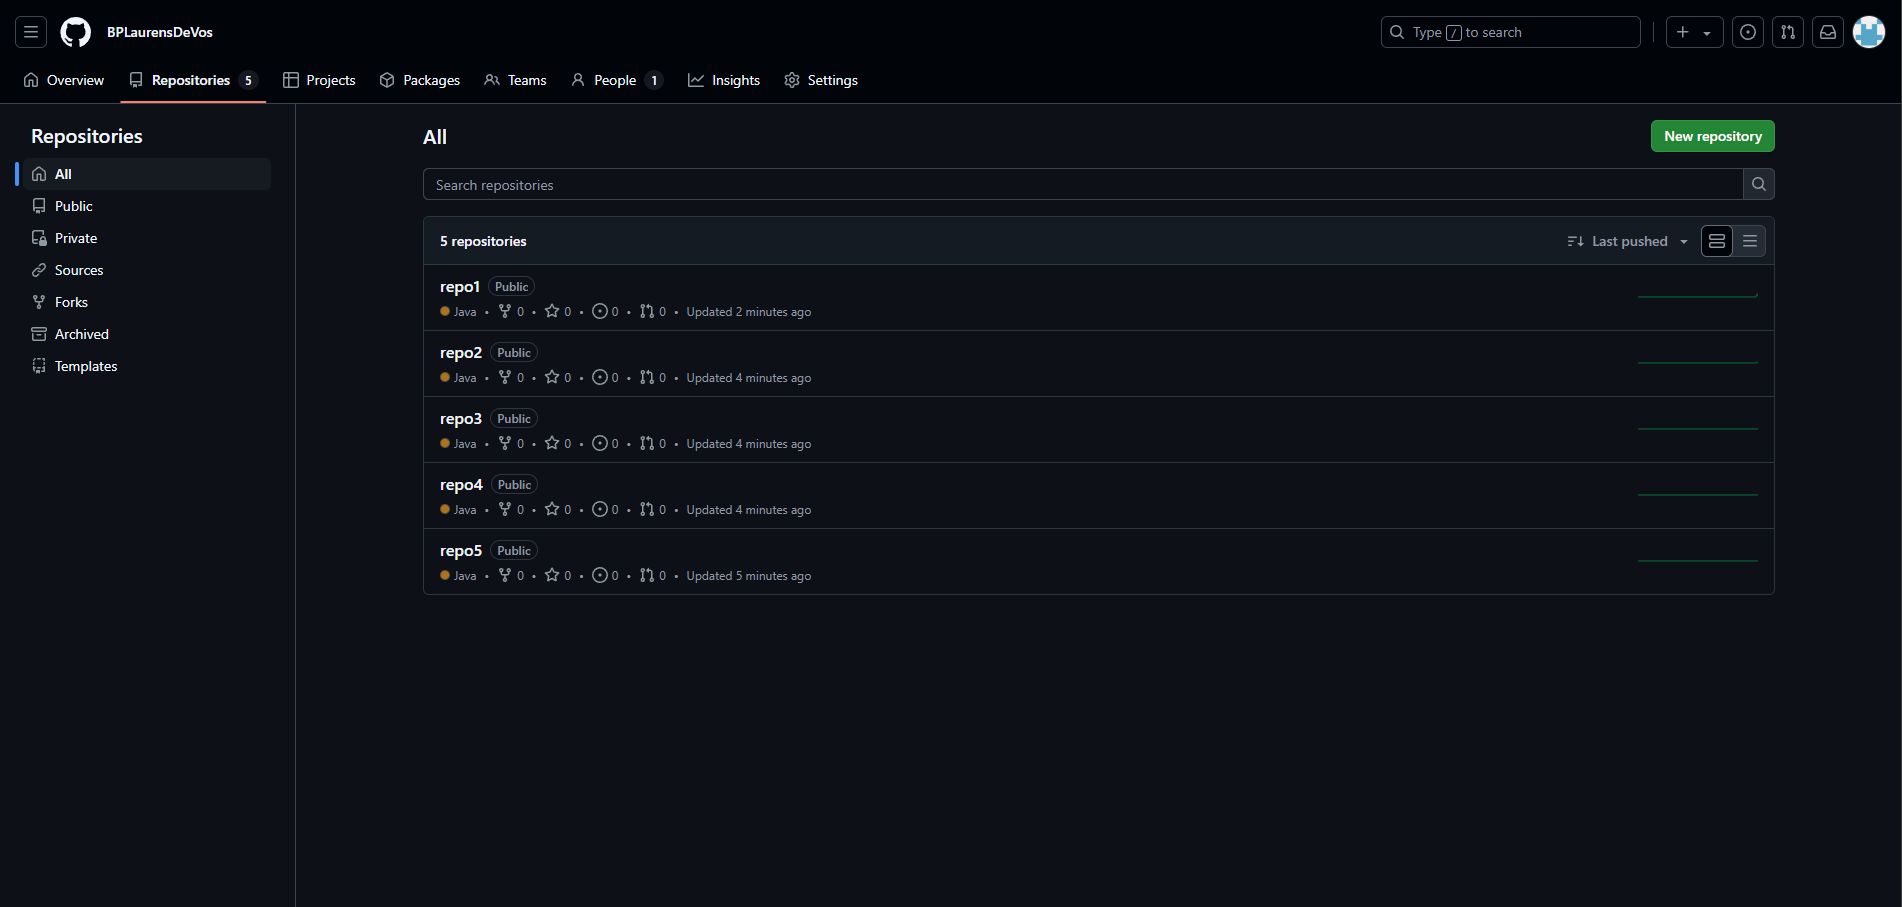
\includegraphics[width=\linewidth]{"C:/Users/laure/Documents/bachelorproef-2024-2025-laurensDeVos/graphics/screenGithubRepo.png"}
    \caption{structuur van alle github repositories}
    \label{fig:repositories}
\end{figure}

\begin{figure}[h!]
    \centering
    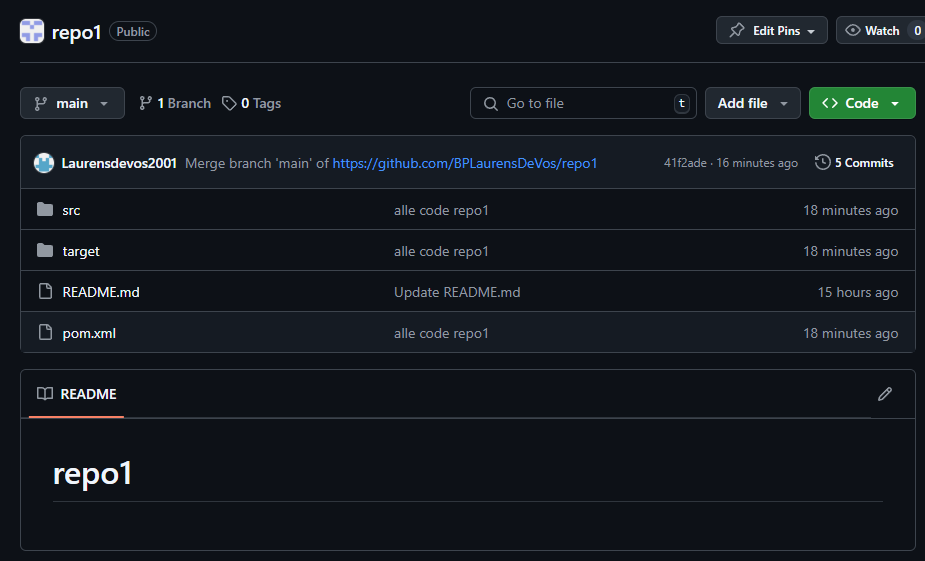
\includegraphics[width=\linewidth]{"C:/Users/laure/Documents/bachelorproef-2024-2025-laurensDeVos/graphics/structuurRepo1.png"}
    \caption{structuur van repo1}
    \label{fig:structuur}
\end{figure}

\ref{fig:repositories}
\ref{fig:structuur}

\subsection{Genereren van de Maven-projecten}
Elk van de vijf repositories is gecreëerd met behulp van de \texttt{maven-archetype-quickstart} template, een standaard template voor Java-projecten in Maven. De volgende commando's zijn gebruikt om een basisproject aan te maken (voor \texttt{Repo1}):

\begin{verbatim}
    mvn archetype:generate "-DgroupId=com.example.repo1" \
    "-DartifactId=repo1" \
    "-DarchetypeArtifactId=maven-archetype-quickstart" \
    "-DinteractiveMode=false"
\end{verbatim}


Het bovenstaande proces is herhaald voor \texttt{Repo2} tot en met \texttt{Repo5}, waarbij de \texttt{groupId} en \texttt{artifactId} telkens zijn aangepast.

\subsection{Afhankelijkheden instellen}
De afhankelijkheden tussen de repositories zijn ingesteld in de \texttt{pom.xml}-bestanden. Zo is \texttt{Repo2} afhankelijk gemaakt van \texttt{Repo1}, terwijl \texttt{Repo3} afhankelijk is van \texttt{Repo2}, enzovoort. Het volgende voorbeeld toont een fragment van de \texttt{pom.xml} van \texttt{Repo2}:

\begin{verbatim}
    <dependencies>
    <dependency>
    <groupId>com.example.repo1</groupId>
    <artifactId>repo1</artifactId>
    <version>1.0-SNAPSHOT</version>
    </dependency>
    </dependencies>
\end{verbatim}

Het configureren van de afhankelijkheden zorgt ervoor dat de build van een repository automatisch de afhankelijkheden downloadt en gebruikt.

\subsection{Toevoegen van dummy code}
Om de functionaliteiten van de repositories te simuleren, is in elke repository eenvoudige Java-code toegevoegd die de afhankelijkheden benut. De codebase is ontworpen om:
\begin{itemize}
    \item De onderlinge afhankelijkheden expliciet te maken.
    \item Te testen of de functionaliteiten correct werken via unit tests.
\end{itemize}

Hieronder volgt een voorbeeld van een simpele klasse in \texttt{Repo1}:

\begin{verbatim}
    package com.example.repo1;
    
    public class Utility {
        public static String getMessage() {
            return "Hello from Repo1!";
        }
    }
\end{verbatim}

Een voorbeeld van een afhankelijkheid in \texttt{Repo2}:

\begin{verbatim}
    package com.example.repo2;
    
    import com.example.repo1.Utility;
    
    public class Service2 {
        public String getServiceMessage() {
            return Utility.getMessage() + " Called by Repo2.";
        }
    }
\end{verbatim}

De volledige broncode is te vinden in de github organisatie \url{https://github.com/BPLaurensDeVos}

\subsection{Unit tests}
In elke repository zijn unit tests toegevoegd om de correctheid van de implementatie te waarborgen. Deze tests zijn geschreven met behulp van JUnit 5, een moderne en uitgebreide testbibliotheek. De volgende code toont een voorbeeld van een unit test in \texttt{Repo2}:

\begin{verbatim}
    package com.example.repo2;
    
    import org.junit.jupiter.api.Test;
    import static org.junit.jupiter.api.Assertions.assertEquals;
    
    public class Service2Test {
        @Test
        public void testGetServiceMessage() {
            Service2 service = new Service2();
            assertEquals("Hello from Repo1! Called by Repo2.", 
            service.getServiceMessage());
        }
    }
\end{verbatim}

De tests worden uitgevoerd met het volgende commando:
\begin{verbatim}
    mvn clean test
\end{verbatim}

\subsection{Lokale installatie en controle}
Na het instellen van de afhankelijkheden en toevoegen van de dummy code zijn de repositories lokaal geïnstalleerd met het volgende commando:
\begin{verbatim}
    mvn clean install
\end{verbatim}

Dit commando genereert de vereiste artefacten (zoals JAR-bestanden) en controleert de correcte werking van de afhankelijkheden.

\begin{figure}[h!]
    \centering
    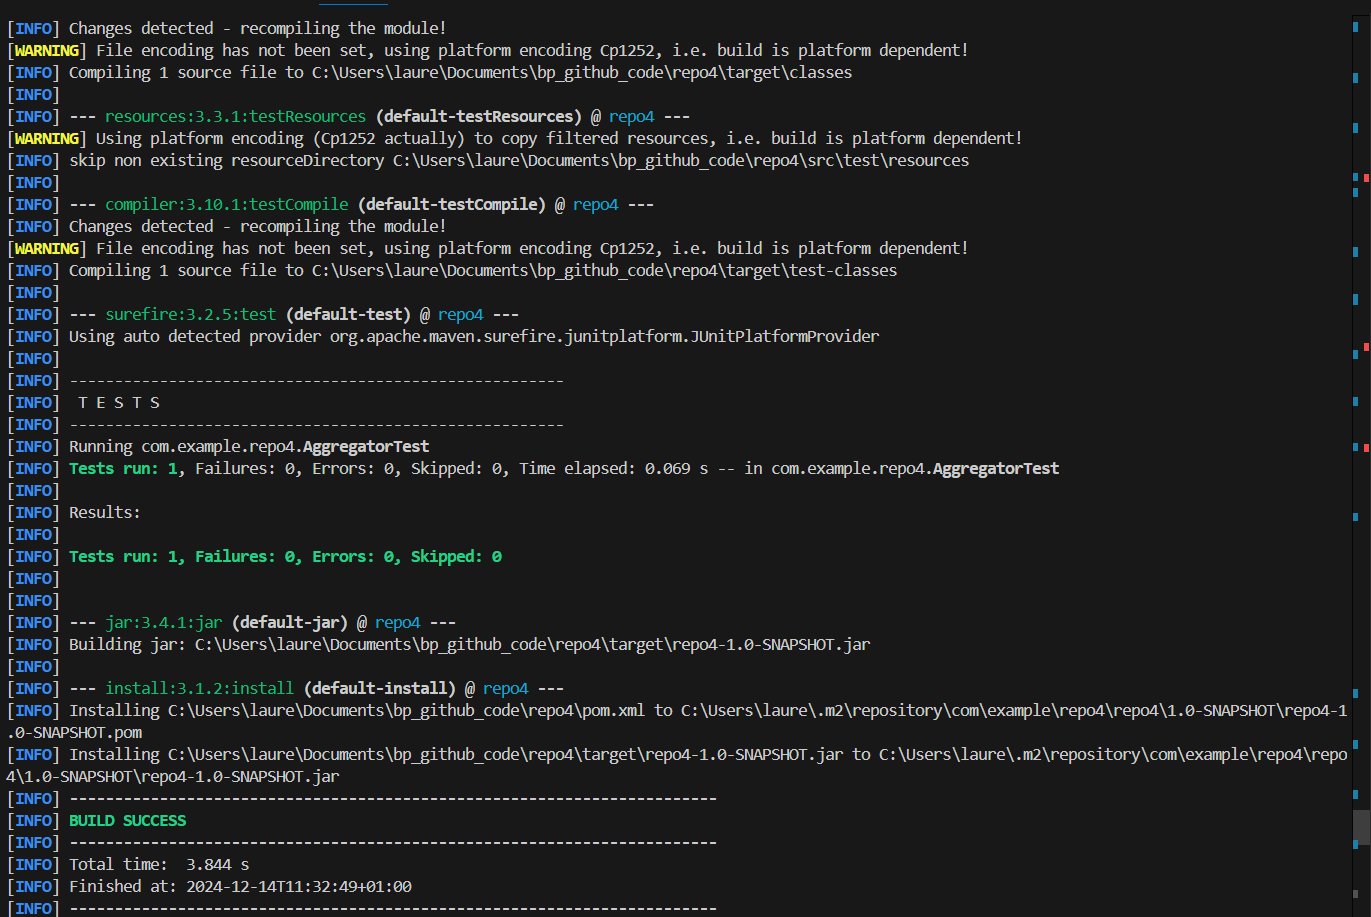
\includegraphics[width=\linewidth]{"C:/Users/laure/Documents/bachelorproef-2024-2025-laurensDeVos/graphics/voorbeeldOutput.png"}
    \caption{De output van 'mvn clean install' in repo4}
    \label{fig:mvncleaninstall}
\end{figure}

De afbeelding \ref{fig:mvncleaninstall} toont de output gegenereerd door vorig commando.


\subsection{GitHub-integratie}
Alle repositories zijn geüpload naar GitHub onder de organisatie \texttt{BPLaurensDeVos}. Een voorbeeld van het pushen van de code naar GitHub:

\begin{verbatim}
    git init
    git remote add origin https://github.com/BPLaurensDeVos/repo1.git
    git add .
    git commit -m "eerste commit repo1"
    git branch -M main
    git push -u origin main --force
\end{verbatim}

\subsection{Conclusie}
Met deze opzet is een solide basis gelegd voor het testen van Jenkins en GitHub Actions. De gekozen structuur en dummy code maken het mogelijk om complexe workflows te simuleren en de tools eerlijk te vergelijken op basis van de gestelde evaluatiecriteria.


\section{Ontwerp en Implementatie van CI/CD-pipelines}

\subsection{Inleiding}
Het opzetten van CI/CD-pipelines in zowel Jenkins als GitHub Actions vormt een cruciaal onderdeel van deze studie. Deze pipelines zijn ontworpen om de workflows van vijf Java-repositories met onderlinge afhankelijkheden te simuleren. Het doel is om de tools te configureren met een identieke structuur en workflow, zodat een eerlijke vergelijking mogelijk is.

De CI/CD-pipelines bestaan uit de volgende stappen:
\begin{itemize}
    \item \textbf{Build}: Het compileren van de Java-code met Maven.
    \item \textbf{Test}: Het uitvoeren van unit tests om de functionaliteit te valideren.
    \item \textbf{Deploy}: Het publiceren van artefacten naar Github Packages.
    \item \text{SonarCloud scan}: Het uitvoeren van code quality checks met SonarCloud.
\end{itemize}

De afhankelijkheden tussen de repositories worden expliciet beheerd, zodat de workflows correct functioneren. In deze sectie worden de implementaties in Jenkins en GitHub Actions apart behandeld.

\subsection{Implementatie van CI/CD met GitHub Actions}

GitHub Actions biedt een native CI/CD-oplossing die naadloos integreert met GitHub. Voor deze Proof-of-Concept werd GitHub Actions gebruikt om pipelines op te zetten voor vijf Java-repositories met onderlinge afhankelijkheden. Elke repository heeft zijn eigen pipeline, waarbij artefacten van andere repositories worden gedownload via GitHub Packages. 

\subsubsection{Doelstellingen van de CI/CD-pipeline}
De GitHub Actions-pipelines zijn ontworpen om:
\begin{itemize}
    \item \textbf{De Java-code te bouwen}: Het compileren van de code in elke repository met behulp van Maven.
    \item \textbf{Unit tests uit te voeren}: JUnit-tests draaien om de functionaliteit van de code te valideren.
    \item \textbf{Artefacten te publiceren}: Gereedgemaakte artefacten (JAR-bestanden) naar GitHub Packages publiceren.
    \item \textbf{Afhankelijkheden te beheren}: Controleren of benodigde artefacten beschikbaar zijn en indien nodig upstream repositories aanroepen.
    \item \textbf{SonarCloud-integratie}: Uitvoeren van code quality checks via SonarCloud.
\end{itemize}

\subsubsection{Voorbereiding van het project} \label{subsec:voorbereidingvanhetproject}

Bij de implementatie van de Proof-of-Concept (PoC) voor het vergelijken van Jenkins en GitHub Actions was een grondige voorbereiding noodzakelijk. Deze voorbereiding omvatte het opzetten van repositories, het configureren van SonarCloud voor kwaliteitsanalyse, en het instellen van de benodigde secrets in GitHub. De stappen in dit proces worden hieronder beschreven.

\begin{enumerate}
    \item \textbf{Aanmaken van repositories}:
    \begin{itemize}
        \item Elk van de vijf repositories (\texttt{Repo1} tot \texttt{Repo5}) werd geconfigureerd in GitHub onder de organisatie \texttt{BPLaurensDeVos}. 
        \item Elke repository bevat:
        \begin{itemize}
            \item Een Maven-project, met een \texttt{pom.xml} die afhankelijkheden en build-configuraties definieert.
            \item Dummy-code om onderlinge afhankelijkheden tussen de repositories te simuleren.
            \item Unit tests geschreven in JUnit 5, die dienen om de functionaliteit van de code te valideren.
        \end{itemize}
    \end{itemize}
    
    \item \textbf{Aanmaken van SonarCloud}:
    SonarCloud werd geïntegreerd om statische code-analyse, kwaliteitsbewaking en beveiligingscontroles uit te voeren. Het proces omvatte:
    \begin{enumerate}
        \item \textbf{Registratie en organisatie-instelling}:
        \begin{itemize}
            \item Een SonarCloud-account werd aangemaakt via \url{https://sonarcloud.io}, gebruikmakend van GitHub-authenticatie.
            \item Een organisatie genaamd \texttt{BPLaurensDeVos} werd opgezet binnen SonarCloud, gekoppeld aan de GitHub-organisatie.
        \end{itemize}
        
        \item \textbf{Projectconfiguratie}:
        \begin{itemize}
            \item Vier van de vijf repositories (Repo2 tot en met Repo5) werden toegevoegd als een project in SonarCloud. 
            \item Voor elk project werd een unieke \texttt{sonar.projectKey} gegenereerd, die wordt gebruikt tijdens de analyse.
        \end{itemize}
        
        \item \textbf{Genereren van een SonarCloud-token}:
        \begin{itemize}
            \item Een token werd aangemaakt in SonarCloud via \texttt{My Account > Security}.
            \item Dit token werd geconfigureerd als een GitHub secret genaamd \texttt{SONAR\_TOKEN} in elk van de vijf repositories.
        \end{itemize}
    \end{enumerate}
    
    \item \textbf{Configureren van GitHub Secrets}:
    Om de CI/CD-pipelines succesvol te laten werken, werden de volgende secrets geconfigureerd in GitHub:
    \begin{itemize}
        \item \texttt{PAT\_TOKEN}: Een Personal Access Token (PAT) werd aangemaakt met de volgende rechten:
        \begin{itemize}
            \item \texttt{read:packages} en \texttt{write:packages} om artefacten te downloaden en uploaden in GitHub Packages.
            \item \texttt{repo} om toegang te krijgen tot de repositories en workflows.
        \end{itemize}
        Het token werd toegevoegd als een GitHub secret met de naam \texttt{PAT\_TOKEN} in elk van de repositories.
        
        \item \texttt{SONAR\_TOKEN}: Een SonarCloud-authenticatietoken werd aangemaakt en geconfigureerd om de SonarCloud-scan te autoriseren. Dit omvatte:
        \begin{itemize}
            \item Het genereren van het token in SonarCloud.
            \item Het toevoegen van het token als een GitHub secret genaamd \texttt{SONAR\_TOKEN} in de organisatie.
        \end{itemize}
    \end{itemize}
\end{enumerate}


In de afbeelding \ref{fig:PATTOKEN} is te zien dat een Personal Acces Token werd aangemaakt in Settings $\rightarrow$ Developer Settings $\rightarrow$ Personal acces tokens $\rightarrow$ Tokens(classic).

\begin{figure}[h!]
    \centering
    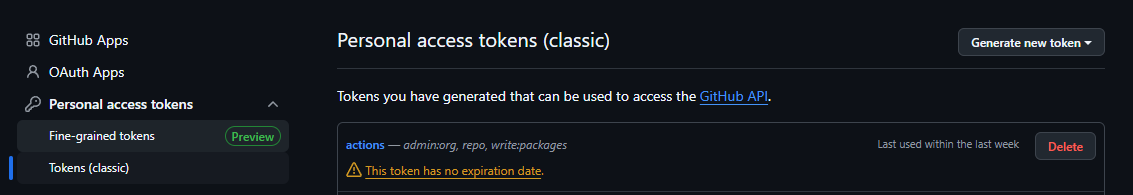
\includegraphics[width=\linewidth]{"C:/Users/laure/Documents/bachelorproef-2024-2025-laurensDeVos/graphics/pat_token.png"}
    \caption{Personal Acces Token.}
    \label{fig:PATTOKEN}
\end{figure}

\begin{figure}[h!]
    \centering
    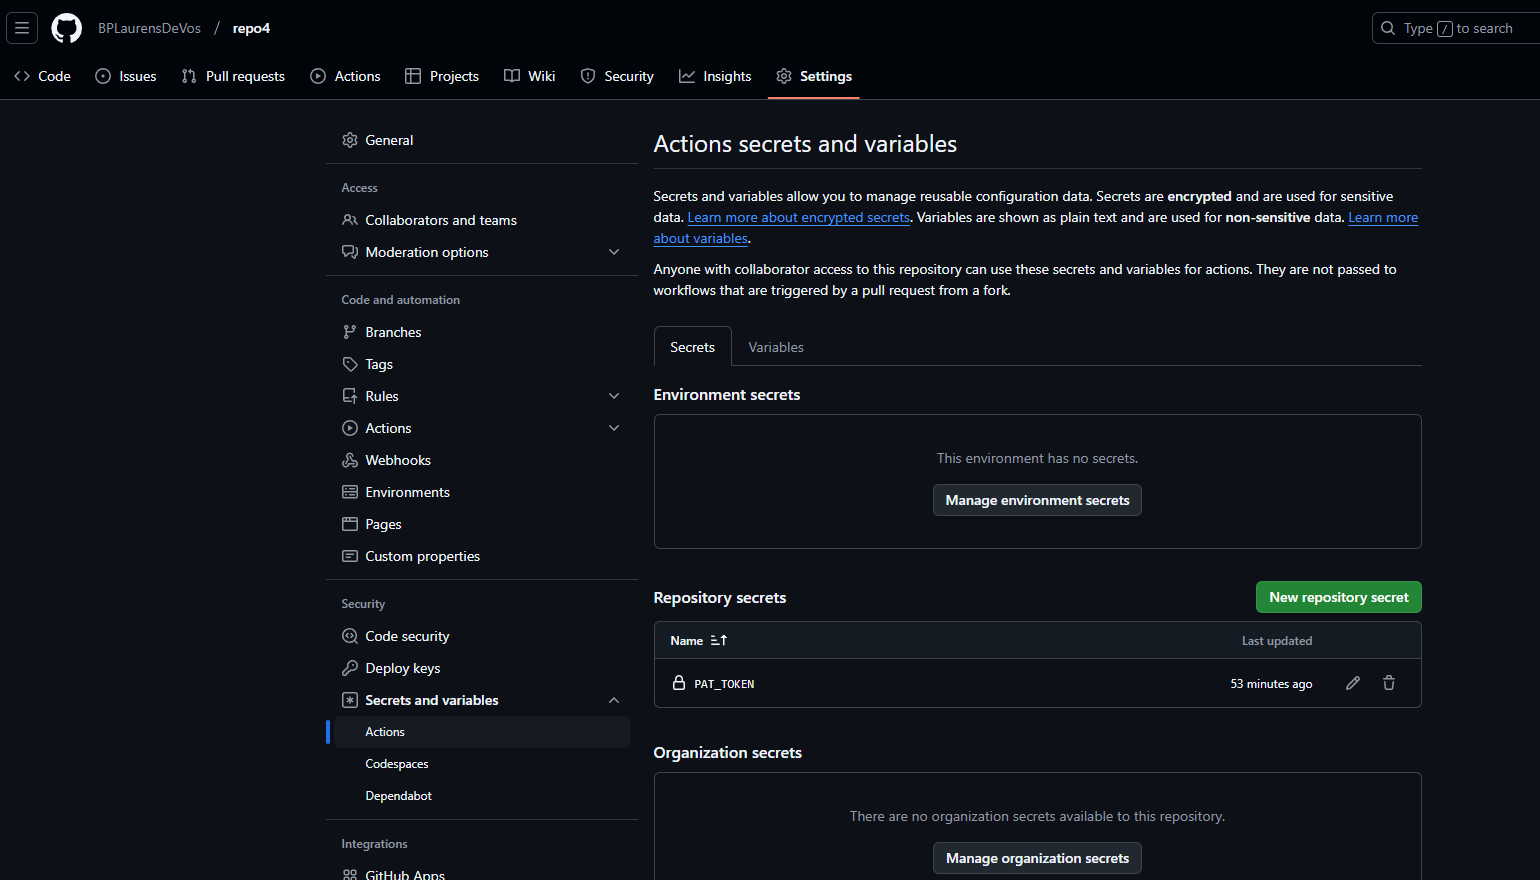
\includegraphics[width=\linewidth]{"C:/Users/laure/Documents/bachelorproef-2024-2025-laurensDeVos/graphics/tokenRepo.png"}
    \caption{Voorbeeld van de token toegevoegd als secret in Repo5.}
    \label{fig:tokenRepo}
\end{figure}

\subsubsection{Workflowconfiguratie in GitHub Actions}

In deze subsubsectie wordt het proces beschreven van het opzetten en configureren van de workflows in GitHub Actions voor de vijf repositories. Elke repository heeft een unieke workflow, gebaseerd op een herbruikbare structuur met specifieke aanpassingen afhankelijk van de afhankelijkheden van de repository.

\paragraph{Algemene structuur van de workflow}
De workflows in GitHub Actions worden gedefinieerd in YAML-bestanden onder de map \texttt{.github/workflows/}. Het basisworkflowbestand bestaat uit de volgende secties:
\begin{enumerate}
    \item \textbf{Triggers}: Bepaalt wanneer de workflow wordt uitgevoerd.
    \item \textbf{Jobs}: Beschrijft de specifieke taken die in de workflow moeten worden uitgevoerd.
    \item \textbf{Environment Configuration}: Voorzien van secrets zoals \texttt{PAT\_TOKEN} en configuratie van Maven.
\end{enumerate}

\paragraph{Triggers}
De workflows worden uitgevoerd bij:
\begin{itemize}
    \item Een \texttt{push} naar de \texttt{main}-branch.
    \item Een \texttt{repository\_dispatch}-event, gebruikt om downstream workflows te activeren.
\end{itemize}

\textbf{Codevoorbeeld:}

\begin{verbatim}
    on:
      push:
        branches:
          - main
      repository_dispatch:
        types:
          - build-artifact
\end{verbatim}

\begin{figure}[h!]
    \centering
    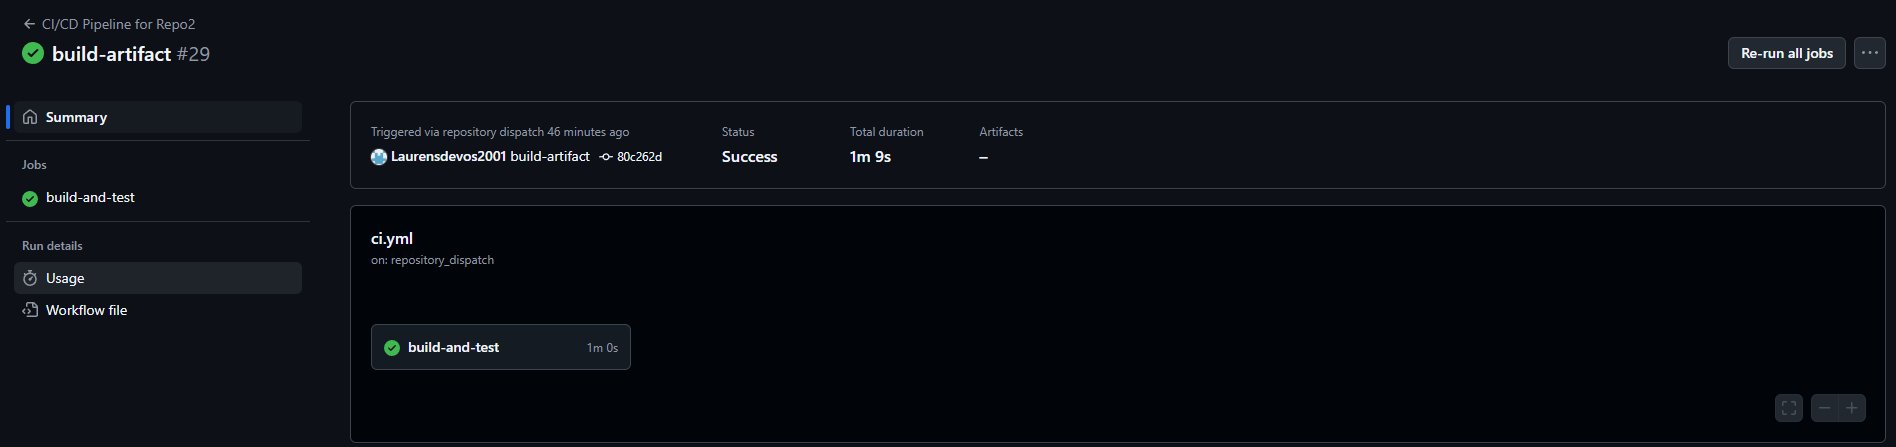
\includegraphics[width=\linewidth]{"C:/Users/laure/Documents/bachelorproef-2024-2025-laurensDeVos/graphics/uitgevoerdeWorkflow.png"}
    \caption{een workflow (repo1) uitgevoerd door \texttt{repository\_dispatch}.}
    \label{fig:uitgevoerdeWorkflow}
\end{figure}

\paragraph{Gedetailleerde beschrijving van de jobs}
De jobs in elke workflow volgen een herbruikbaar patroon, met unieke stappen voor afhankelijkheden. Hieronder volgt een voorbeeld van de workflow voor \texttt{Repo1}.

\subparagraph{Stap 1: Checkout van de repository}
Met behulp van de \texttt{actions/checkout@v3}-actie wordt de meest recente code opgehaald uit de GitHub-repository.

\begin{verbatim}
    - name: Checkout Repository
      uses: actions/checkout@v3
\end{verbatim}

\begin{figure}[h!]
    \centering
    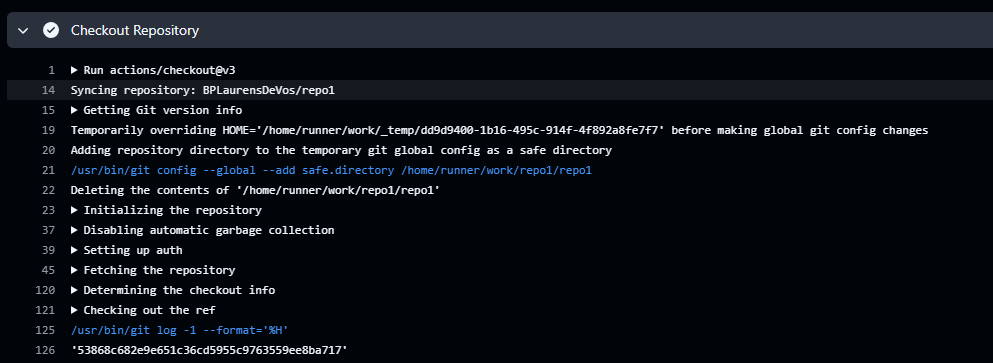
\includegraphics[width=\linewidth]{"C:/Users/laure/Documents/bachelorproef-2024-2025-laurensDeVos/graphics/checkout1.png"}
    \caption{Succesvolle uitvoer van de Checkout Repository job}
    \label{fig:check1}
\end{figure}

\subparagraph{Stap 2: Configureren van JDK 17}
De actie \texttt{actions/setup-java@v3} configureert Java 17, een vereiste voor het Maven-buildproces.

\begin{verbatim}
    - name: Set up JDK 17
      uses: actions/setup-java@v3
      with:
        java-version: 17
        distribution: 'temurin'
\end{verbatim}

\begin{figure}[h!]
    \centering
    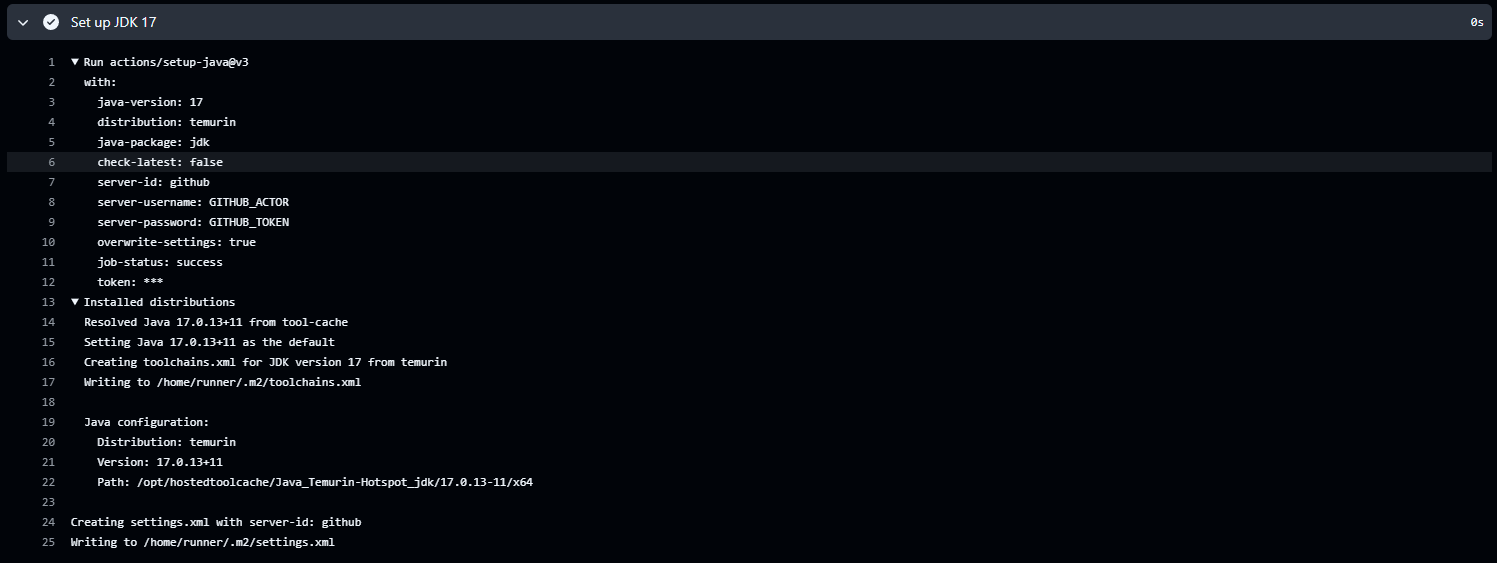
\includegraphics[width=\linewidth]{"C:/Users/laure/Documents/bachelorproef-2024-2025-laurensDeVos/graphics/java1.png"}
    \caption{Succesvolle uitvoer van de Set up JDK 17 Repository job}
\end{figure}

\subparagraph{Stap 3: Build en Test}
De code wordt gebouwd en de tests worden uitgevoerd met behulp van Maven-commando's. Dit valideert de functionaliteit van de code.

\begin{verbatim}
    - name: Build and Test
      run: mvn clean package
\end{verbatim}

\begin{figure}[h!]
    \centering
    \includegraphics[width=\linewidth]{"C:/Users/laure/Documents/bachelorproef-2024-2025-laurensDeVos/graphics/Buildpackage1.png"}
    \caption{Build succes toont aan dat de de applicatie is opgebouwd en getest}
\end{figure}


\subparagraph{Stap 4: Publiceren naar GitHub Packages}
Artefacten (zoals JAR-bestanden) worden gepubliceerd naar GitHub Packages met behulp van het \texttt{mvn deploy}-commando. 

\begin{verbatim}
    - name: Publish to GitHub Packages
      run: mvn deploy
      env:
        GITHUB_ACTOR: ${{ github.actor }}
        GITHUB_TOKEN: ${{ secrets.PAT_TOKEN }}
\end{verbatim}

\begin{figure}[h!]
    \centering
    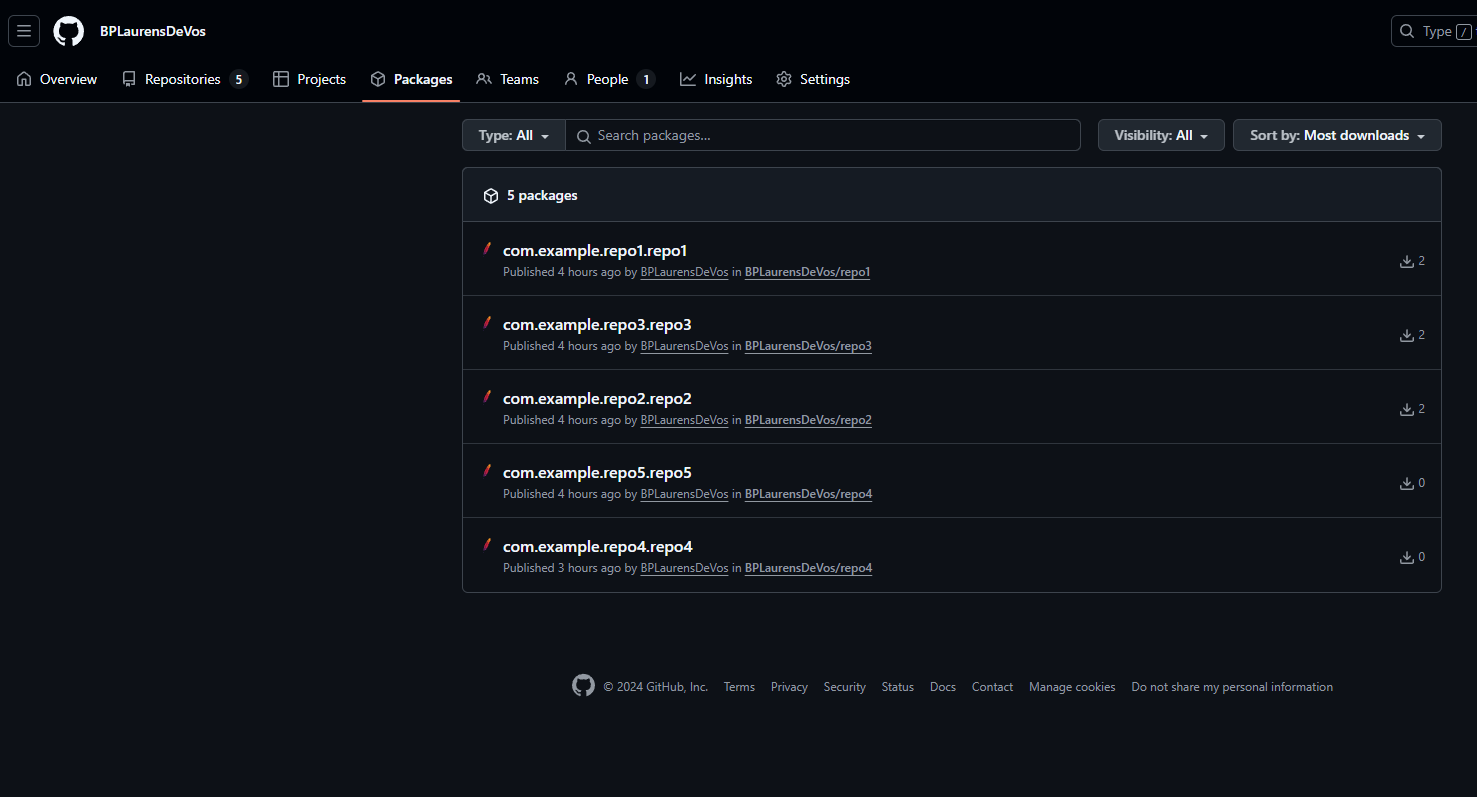
\includegraphics[width=\linewidth]{"C:/Users/laure/Documents/bachelorproef-2024-2025-laurensDeVos/graphics/packages.png"}
    \caption{Alle artifacts zijn te vinden in de GitHub organisatie (BPLaurensDeVos) onder $\rightarrow$ Packages}
\end{figure}

\paragraph{Complete workflow voor Repo1}
Hieronder volgt het volledige YAML-bestand van de workflow voor \texttt{Repo1}:

\begin{verbatim}
    name: CI/CD Pipeline for Repo1
    
    on:
      push:
        branches:
          - main
      repository_dispatch:
        types:
          - build-artifact
    
    jobs:
      build-and-test:
        runs-on: ubuntu-latest
        steps:
          - name: Checkout Repository
            uses: actions/checkout@v3
    
          - name: Set up JDK 17
            uses: actions/setup-java@v3
            with:
              java-version: 17
              distribution: 'temurin'
    
          - name: Build and Test
            run: mvn clean package
    
          - name: Publish to GitHub Packages
            run: mvn deploy
            env:
              GITHUB_ACTOR: ${{ github.actor }}
              GITHUB_TOKEN: ${{ secrets.PAT_TOKEN }}
\end{verbatim}

\begin{figure}[h!]
    \centering
    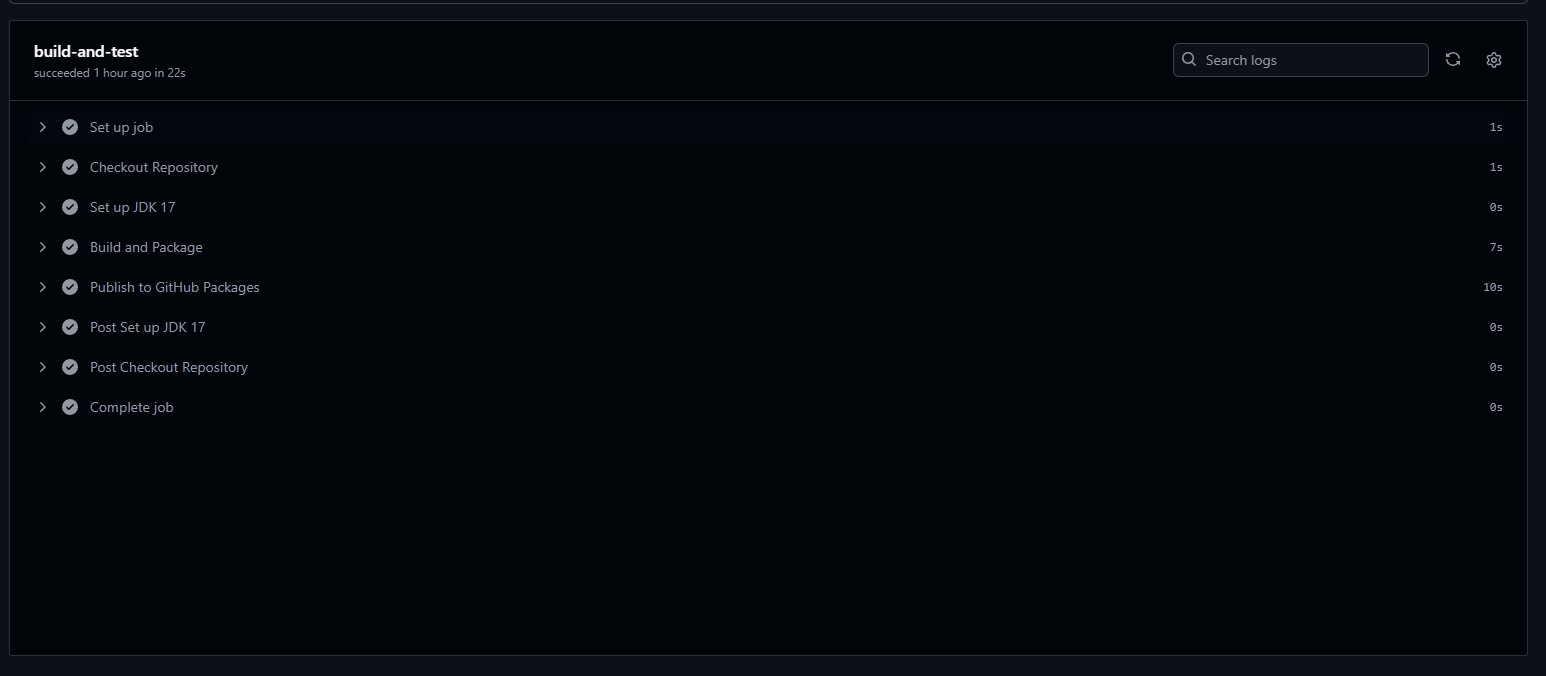
\includegraphics[width=\linewidth]{"C:/Users/laure/Documents/bachelorproef-2024-2025-laurensDeVos/graphics/Repo1Geslaagd.png"}
    \caption{Overzicht van een succesvolle uitvoering van de workflow in \texttt{Repo1}. Elke job is voltooid, zoals aangegeven door de vinkjes.}
\end{figure}

\paragraph{Specifieke workflows voor downstream repositories}
Repositories zoals \texttt{Repo2} tot \texttt{Repo5} vereisen aanvullende configuraties vanwege hun afhankelijkheden. Voor deze repositories moet eerst worden gecontroleerd of de artefacten van de bijbehorende afhankelijkheden beschikbaar zijn in de GitHub Package Registry. Indien de benodigde artefacten niet beschikbaar zijn, wordt de workflow van de afhankelijke repository gestart via een \texttt{repository\_dispatch}-event om de artefacten alsnog te genereren.

\subparagraph{1. Controleren van artefactbeschikbaarheid}
Om ervoor te zorgen dat de build van een repository correct kan worden uitgevoerd, moeten alle benodigde artefacten van afhankelijkheden beschikbaar zijn in GitHub Packages. Dit wordt gedaan door een HTTP-verzoek uit te voeren naar het specifieke artefact in de package registry van GitHub. De \texttt{curl}-tool wordt gebruikt om een statuscode te verkrijgen die aangeeft of het artefact beschikbaar is.

\begin{itemize} 
    \item Statuscode 200: Het artefact is beschikbaar, wat betekent dat de afhankelijkheid succesvol kan worden gedownload en gebruikt. \item Andere statuscodes: Het artefact is niet beschikbaar, wat betekent dat de workflow van de upstream repository moet worden gestart om het artefact te genereren en te publiceren. 
\end{itemize}

\textbf{Deel van de code in Repo2}:

\begin{verbatim}
    - name: Check Repo1 Artifact Availability
      run: |
            STATUS_CODE=$(curl -L -u ${{ github.actor }}:${{ secrets.PAT_TOKEN }} \
                -s \
                -o /dev/null \
                -w "%{http_code}" \
                https://maven.pkg.github.com/BPLaurensDeVos/repo1/com/example/repo1/repo1/1.0/repo1-1.0.jar)
        echo "Artifact Status Code: $STATUS_CODE"
        echo "repo1_status_code=$STATUS_CODE" >> $GITHUB_ENV
\end{verbatim}

\begin{figure}[h!]
    \centering
    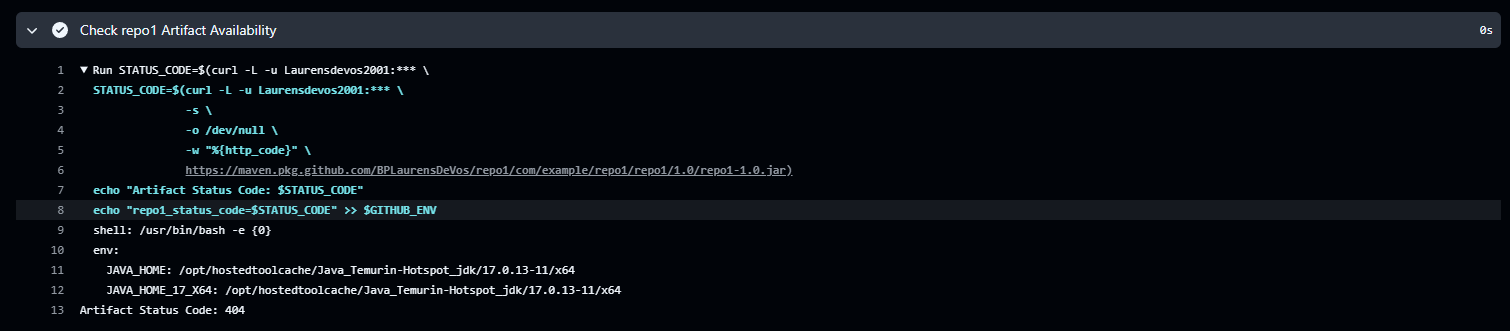
\includegraphics[width=\linewidth]{"C:/Users/laure/Documents/bachelorproef-2024-2025-laurensDeVos/graphics/status404.png"}
    \caption{Voorbeeld uit repo2 waar het artefact niet gevonden wordt en Status Code 404 wordt gegeven. }
\end{figure}

\begin{figure}[h!]
    \centering
    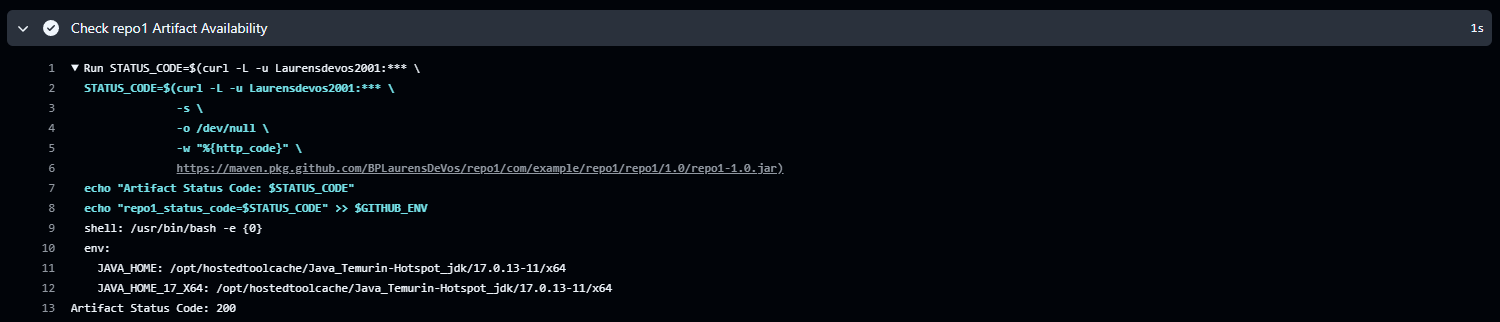
\includegraphics[width=\linewidth]{"C:/Users/laure/Documents/bachelorproef-2024-2025-laurensDeVos/graphics/status200.png"}
    \caption{Voorbeeld uit repo2 waar het artefact wel gevonden wordt en Status Code 200 wordt gegeven. }
\end{figure}

\subparagraph{2. Triggeren van upstream workflows}
Wanneer een afhankelijk artefact niet beschikbaar is in GitHub Packages, moet de workflow van de upstream repository worden gestart. Dit gebeurt door een \texttt{repository\_dispatch}-event te versturen met behulp van de \texttt{curl}-tool. Dit mechanisme zorgt ervoor dat downstream repositories niet vastlopen door ontbrekende afhankelijkheden, maar in plaats daarvan de benodigde artefacten actief opvragen.

\textbf{Deel van de code in Repo2}:

\begin{verbatim}
    - name: Trigger Repo1 if Artifact is Missing
      if: env.repo1_status_code != '200'
      run: |
        curl -X POST \
        -H "Accept: application/vnd.github.v3+json" \
        -H "Authorization: token ${{ secrets.PAT_TOKEN }}" \
           https://api.github.com/repos/BPLaurensDeVos/repo1/dispatches \
        -d '{"event_type":"build-artifact"}'
\end{verbatim}

\begin{figure}[h!]
    \centering
    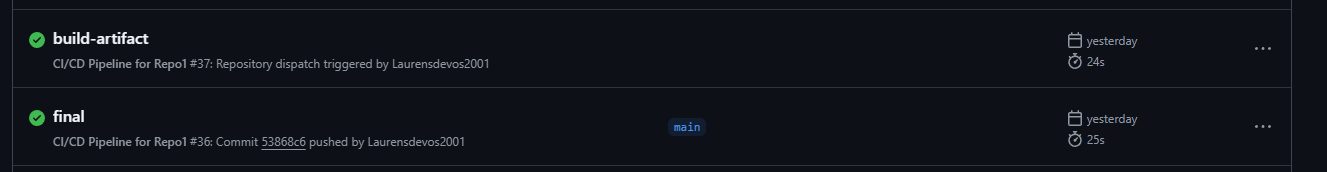
\includegraphics[width=\linewidth]{"C:/Users/laure/Documents/bachelorproef-2024-2025-laurensDeVos/graphics/trigger1.png"}
    \caption{Overzicht van twee workflow-runs: de eerste is gestart door een \texttt{repository\_dispatch}-event met de \texttt{build-artifact}-trigger, terwijl de tweede is gestart door een commit naar de \texttt{main}-branch.}
\end{figure}

\subparagraph{3. Wachten tot het artefact gepubliceerd is}
Nadat de workflow van een upstream repository is geactiveerd, is het noodzakelijk om te wachten totdat het benodigde artefact beschikbaar is in GitHub Packages. Dit voorkomt dat de downstream workflow mislukt vanwege ontbrekende afhankelijkheden. De wachttijd wordt iteratief verhoogd bij de repositories aangezien repo5 mogelijks moet wachten op alle voorgaande repositories en repo2 enkel op repo1.

\textbf{Waarom wachten?}

\begin{itemize} 
    \item Een \texttt{repository\_dispatch}-event start de workflow in een upstream repository, maar het bouwen en publiceren van een artefact kost tijd. 
    \item Zonder een wachtmechanisme zou de downstream workflow direct doorgaan, wat leidt tot fouten als het artefact nog niet beschikbaar is. 
\end{itemize}

\textbf{Voorbeeld uit de workflow van Repo2}:

\begin{verbatim}
      - name: Wait for Repo1 Artifact to be Published
        if: env.repo1_status_code != '200'
        run: |
            echo "Waiting for Repo1 artifact to be published..."
            sleep 30
\end{verbatim}

\textbf{Voorbeeld uit de workflow van Repo5}:

\begin{verbatim}
    - name: Wait for Repo1 Artifact to be Published
    if: env.repo1_status_code != '200'
    run: |
        echo "Waiting for Repo1 artifact to be published..."
        sleep 180
\end{verbatim}

\subparagraph{4. Opnieuw controleren van artefactbeschikbaarheid}
Nadat de workflow van een upstream repository is uitgevoerd, wordt gecontroleerd of het artefact nu beschikbaar is in GitHub Packages. Deze tweede controle bepaalt of de workflow kan doorgaan of moet worden afgebroken wegens ontbrekende afhankelijkheden.

\textbf{Belang van deze stap}:

\begin{itemize} 
    \item Zorgt ervoor dat de workflow alleen doorgaat wanneer alle benodigde artefacten beschikbaar zijn. 
    \item Minimaliseert het risico op fouten verderop in het proces door afhankelijkheden tijdig te valideren. 
\end{itemize}

\textbf{Voorbeeld uit de workflow van Repo2}:

\begin{verbatim}
      - name: Recheck Artifact Availability
        if: env.repo1_status_code != '200'
        id: recheck-artifact
        run: |
            STATUS_CODE=$(curl -L -u ${{ github.actor }}:${{        secrets.PAT_TOKEN }} \
                -s \
                -o /dev/null \
                -w "%{http_code}" \
                https://maven.pkg.github.com/BPLaurensDeVos/repo1/com/example/repo1/repo1/1.0/repo1-1.0.jar)
            echo "Rechecked Artifact Status Code: $STATUS_CODE"
            echo "repo1_recheck_status_code=$STATUS_CODE" >> $GITHUB_ENV
\end{verbatim}

\subparagraph{5. Falen van de workflow}
Als na de tweede controle blijkt dat het benodigde artefact nog steeds niet beschikbaar is in GitHub Packages, wordt de workflow bewust gestopt. Dit voorkomt dat de pipeline verdergaat zonder de vereiste afhankelijkheden, wat later tot build- of runtime-fouten zou kunnen leiden.

\textbf{Voorbeeld uit de workflow van Repo2}:

\begin{verbatim}
      - name: Fail Workflow if Artifact Still Missing
        if: env.repo1_status_code != '200' && env.repo1_recheck_status_code != '200'
        run: |
            echo "Artifact still missing after waiting. Failing workflow..."
            exit 1
\end{verbatim}

\subparagraph{6. Configureren van Maven}
Om ervoor te zorgen dat Maven geauthenticeerd kan communiceren met GitHub Packages, wordt in de workflow dynamisch een aangepaste \texttt{settings.xml}-configuratie gegenereerd. Deze configuratie bevat de authenticatiegegevens van de gebruiker en zorgt ervoor dat Maven toegang heeft tot de package repositories.

\begin{verbatim}
      - name: Configure Maven to Use GitHub Packages
        if: env.repo1_status_code == '200' ||                          env.repo1_recheck_status_code == '200'
        run: |
            mkdir -p ~/.m2
            echo "<settings xmlns='http://maven.apache.org/SETTINGS/1.0.0'
                xmlns:xsi='http://www.w3.org/2001/XMLSchema-instance'
                xsi:schemaLocation='http://maven.apache.org/SETTINGS/1.0.0 https://maven.apache.org/xsd/settings-1.0.0.xsd'>
                <servers>
                    <server>
                        <id>github</id>
                        <username>${{ github.actor }}</username>
                        <password>${{ secrets.PAT_TOKEN }}</password>
                    </server>
                </servers>
              </settings>" > ~/.m2/settings.xml
            cat ~/.m2/settings.xml
\end{verbatim}

Bij \texttt{Repo5} is de configuratie complexer omdat authenticatie vereist is om artefacten van andere repositories te kunnen ophalen. De juiste \texttt{id}'s voor deze repositories worden gespecificeerd in de \texttt{pom.xml}-configuratie van \texttt{Repo5}. De code in de workflow Repo5 is te zien in afbeelding \ref{fig:packages5}.

\begin{figure}[h!]
    \centering
    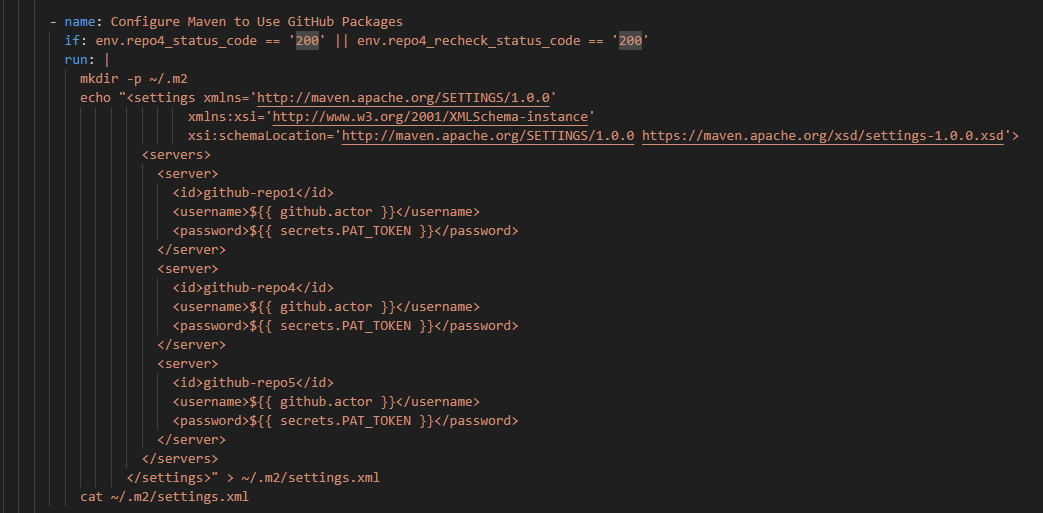
\includegraphics[width=\linewidth]{"C:/Users/laure/Documents/bachelorproef-2024-2025-laurensDeVos/graphics/packages5.png"}
    \label{fig:packages5}
\end{figure}

\subparagraph{7. SonarCloud code quality scan}
Om de kwaliteit van de code te waarborgen en beveiligingsproblemen vroegtijdig te detecteren, wordt een statische code-analyse uitgevoerd met behulp van SonarCloud. Deze stap zorgt ervoor dat de repository voldoet aan vooraf gedefinieerde kwaliteitsstandaarden en maakt eventuele technische schulden of kwetsbaarheden inzichtelijk.

\textbf{Belang van deze stap}:
\begin{itemize}
    \item Voorkomt dat slechte codekwaliteit wordt geïntegreerd in de repository.
    \item Identificeert beveiligingslekken en mogelijke bugs.
    \item Bewaakt de onderhoudbaarheid van de codebase door duplicatie en complexe code te minimaliseren.
\end{itemize}

\textbf{Configuratie in de workflow van Repo2}:
De SonarCloud-scan wordt uitgevoerd met behulp van Maven Sonar Plugin. Deze actie gebruikt de eerder ingestelde \texttt{SONAR\_TOKEN} voor authenticatie en maakt gebruik van de instellingen die in de \texttt{pom.xml} zijn opgenomen.

\begin{verbatim}
    - name: SonarCloud Scan
      if: env.repo1_status_code == '200' || env.repo1_recheck_status_code == '200'
      env:
        SONAR_TOKEN: ${{ secrets.SONAR_TOKEN }}
      run: |
        mvn sonar:sonar -Dsonar.login=${{ secrets.SONAR_TOKEN }}
\end{verbatim}

\subsubsection{Configuratie van de \texttt{pom.xml}}
Naast de \texttt{settings.xml} speelt de \texttt{pom.xml} een centrale rol in de configuratie van de Maven-builds en afhankelijkheden. Voor elk van de repositories bevat de \texttt{pom.xml} de volgende onderdelen:

\paragraph{Afhankelijkheden}
De afhankelijkheden van andere repositories worden gedefinieerd in de sectie \texttt{<dependencies>}. Bijvoorbeeld:

\texttt{Repo2}, dat afhankelijk is van \texttt{Repo1}:
\begin{verbatim}
    <dependencies>
      <dependency>
        <groupId>com.example.repo1</groupId>
        <artifactId>repo1</artifactId>
        <version>1.0</version>
      </dependency>
    </dependencies>
\end{verbatim}

\begin{itemize}
    \item \texttt{<groupId>} en \texttt{<artifactId>} verwijzen naar de unieke identificatie van de artefacten.
    \item \texttt{<version>} specificeert de gewenste versie van het artefact.
\end{itemize}

\paragraph{Repositories}
Om artefacten uit GitHub Packages op te halen, worden de relevante repositories gedefinieerd in de \texttt{<repositories>}-sectie:

Voorbeeldconfiguratie:
\begin{verbatim}
    <repositories>
      <repository>
        <id>github</id>
        <url>https://maven.pkg.github.com/BPLaurensDeVos/repo1</url>
      </repository>
    </repositories>
\end{verbatim}

\paragraph{DistributionManagement} 
De \texttt{<distributionManagement>}-sectie in de \texttt{pom.xml} specificeert de locatie waar het artefact van de repository moet worden gepubliceerd. Dit is vooral belangrijk voor het correct opslaan van artefacten in GitHub Packages.

Voorbeeldconfiguratie in Repo2:
\begin{verbatim} 
    <distributionManagement>
      <repository> 
        <id>github</id> <url>https://maven.pkg.github.com/BPLaurensDeVos/repo2</url>
      </repository> </distributionManagement> 
    </distributionManagement>
\end{verbatim}

\begin{itemize} 
    \item \texttt{<id>} moet overeenkomen met de configuratie in de \texttt{settings.xml} om correcte authenticatie te garanderen.
    \item \texttt{<url>} verwijst naar de locatie in GitHub Packages waar het artefact moet worden opgeslagen. 
\end{itemize}

Deze configuratie zorgt ervoor dat artefacten na het buildproces automatisch naar de juiste locatie in GitHub Packages worden gepubliceerd, zodat ze beschikbaar zijn voor downstream repositories.

\paragraph{Build-configuratie}
Het buildproces wordt aangepast met behulp van plugins, zoals de Maven Compiler Plugin en de SonarCloud Maven Plugin:

\begin{verbatim}
    <build>
      <plugins>
        <plugin>
            <groupId>org.apache.maven.plugins</groupId>
            <artifactId>maven-compiler-plugin</artifactId>
            <version>3.10.1</version>
            <configuration>
              <source>17</source>
              <target>17</target>
            </configuration>
        </plugin>
        <plugin>
          <groupId>org.sonarsource.scanner.maven</groupId>
          <artifactId>sonar-maven-plugin</artifactId>
          <version>3.9.1.2184</version>
        </plugin>
      </plugins>
    </build>
\end{verbatim}

\paragraph{Properties}
De \texttt{<properties>}-sectie bevat configuraties voor zowel de Maven Compiler Plugin als de SonarCloud integratie. Deze instellingen zorgen voor consistentie in het buildproces en een correcte verbinding met SonarCloud:

\begin{verbatim}
    <properties>
      <maven.compiler.source>17</maven.compiler.source>
      <maven.compiler.target>17</maven.compiler.target>
      <sonar.projectKey>BPLaurensDeVos_repo2</sonar.projectKey>
      <sonar.organization>bplaurensdevos</sonar.organization>
      <sonar.host.url>https://sonarcloud.io</sonar.host.url>
    </properties>
\end{verbatim}

De Java-compiler gebruikt versie 17 voor zowel broncode als doelcode, terwijl SonarCloud wordt geconfigureerd met een unieke projectkey, organisatie en host-URL.

\paragraph{Relatie tussen \texttt{settings.xml} en \texttt{pom.xml}}
De \texttt{settings.xml} zorgt voor de authenticatie en maakt toegang tot de repositories mogelijk, terwijl de \texttt{pom.xml} de structuur, afhankelijkheden en build-definities van het project specificeert. Samen vormen deze bestanden de kern van de Maven-configuratie.


\subsection{Implementatie van CI/CD met Jenkins}

\subsubsection{Inleiding}

Jenkins is een open-source automation server die wordt gebruikt om softwareontwikkeling te versnellen door Continuous Integration en Continuous Deployment (CI/CD)-processen te automatiseren. Het biedt een uitgebreide set aan functionaliteiten via plug-ins en ondersteunt een breed scala aan technologieën, waaronder Maven, SonarQube en Docker.

In deze Proof-of-Concept (PoC) wordt Jenkins geëvalueerd om te bepalen hoe goed het aansluit bij de behoeften van DocShifter in termen van prestaties, beveiliging en integratie met bestaande systemen. Jenkins wordt vergeleken met GitHub Actions, waarbij beide tools worden gebruikt om identieke workflows uit te voeren. Het doel is om een eerlijk en grondig inzicht te krijgen in de sterke en zwakke punten van Jenkins binnen de context van deze simulatie.

\subsubsection{Doelstellingen van de CI/CD-pipeline in Jenkins}

De Jenkins CI/CD-pipelines hebben dezelfde doelstellingen als die in GitHub Actions:
\begin{itemize}
    \item \textbf{Build}: Het compileren van de Java-code met Maven.
    \item \textbf{Test}: Het uitvoeren van unit tests geschreven in JUnit 5.
    \item \textbf{Deploy}: Het publiceren van artefacten naar GitHub Packages.
    \item \textbf{Afhankelijkheden beheren}: Upstream repositories triggeren indien hun artefacten ontbreken.
    \item \textbf{SonarCloud-integratie}: Codekwaliteit controleren en technische schulden identificeren.
\end{itemize}

\subsubsection{Installatie en Configuratie van Jenkins}
\subsubsection{Installatie van Jenkins}

Jenkins is lokaal geïnstalleerd in een Docker-container om een flexibele en reproduceerbare testomgeving te bieden. De installatie werd uitgevoerd met de volgende stappen:

\begin{enumerate}
    \item \textbf{Installeren van Docker Desktop}:
    Docker Desktop werd geïnstalleerd op een Windows-machine. Dit biedt een gemakkelijke manier om Docker-containers te beheren en te starten.
    \item \textbf{Pullen van de Jenkins Docker Image}:
    Het officiële Jenkins Docker-image werd gedownload met het volgende commando:
    \begin{verbatim}
        docker pull jenkins/jenkins:lts
    \end{verbatim}
    \item \textbf{Starten van de Jenkins-container}:
    De container werd gestart met het volgende commando:
    \begin{verbatim}
        docker run -d --name jenkins -p 8080:8080 -p 50000:50000 \
        -v jenkins_home:/var/jenkins_home jenkins/jenkins:lts
    \end{verbatim}
    \item \textbf{Toegang tot de Jenkins webinterface}:
    Na het starten van de container werd Jenkins toegankelijk via \url{http://localhost:8080}.
    \item \textbf{Initialisatie van Jenkins}:
    Tijdens de eerste keer opstarten genereert Jenkins een initiële admin-wachtwoord. Dit wachtwoord werd opgehaald met het volgende commando:
    \begin{verbatim}
        docker exec jenkins cat /var/jenkins_home/secrets/initialAdminPassword
    \end{verbatim}
    \item \textbf{Installeren van plug-ins}:
    Tijdens de eerste configuratie werden de aanbevolen plug-ins automatisch geïnstalleerd. Deze omvatten onder andere:
    \begin{itemize}
        \item \texttt{Pipeline}.
        \item \texttt{GitHub}.
    \end{itemize}
    Na deze automatische installatie werden de volgende aanvullende plug-ins handmatig geïnstalleerd:
    \begin{itemize}
        \item \texttt{Maven Integration} (voor het configureren van Maven-builds).
        \item \texttt{SonarQube Scanner for Jenkins} (voor integratie met SonarCloud).
    \end{itemize}
\end{enumerate}

\begin{figure}[h!]
    \centering
    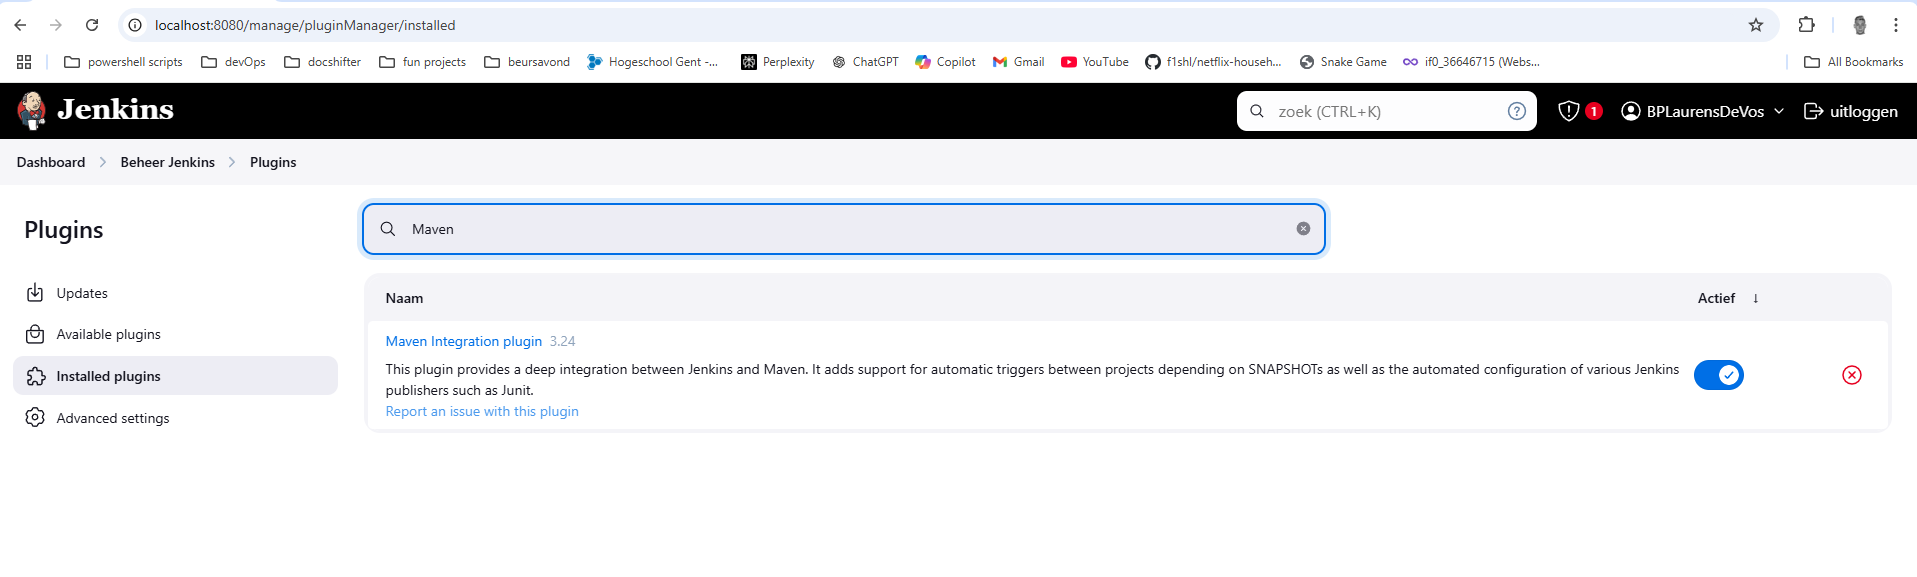
\includegraphics[width=\linewidth]{"C:/Users/laure/Documents/bachelorproef-2024-2025-laurensDeVos/graphics/JenkinsPluginMaven.png"}
    \caption{Maven integration plugin geïnstalleerd op de Jenkins server}
    \label{fig:install_Maven}
\end{figure}

\begin{figure}[h!]
    \centering
    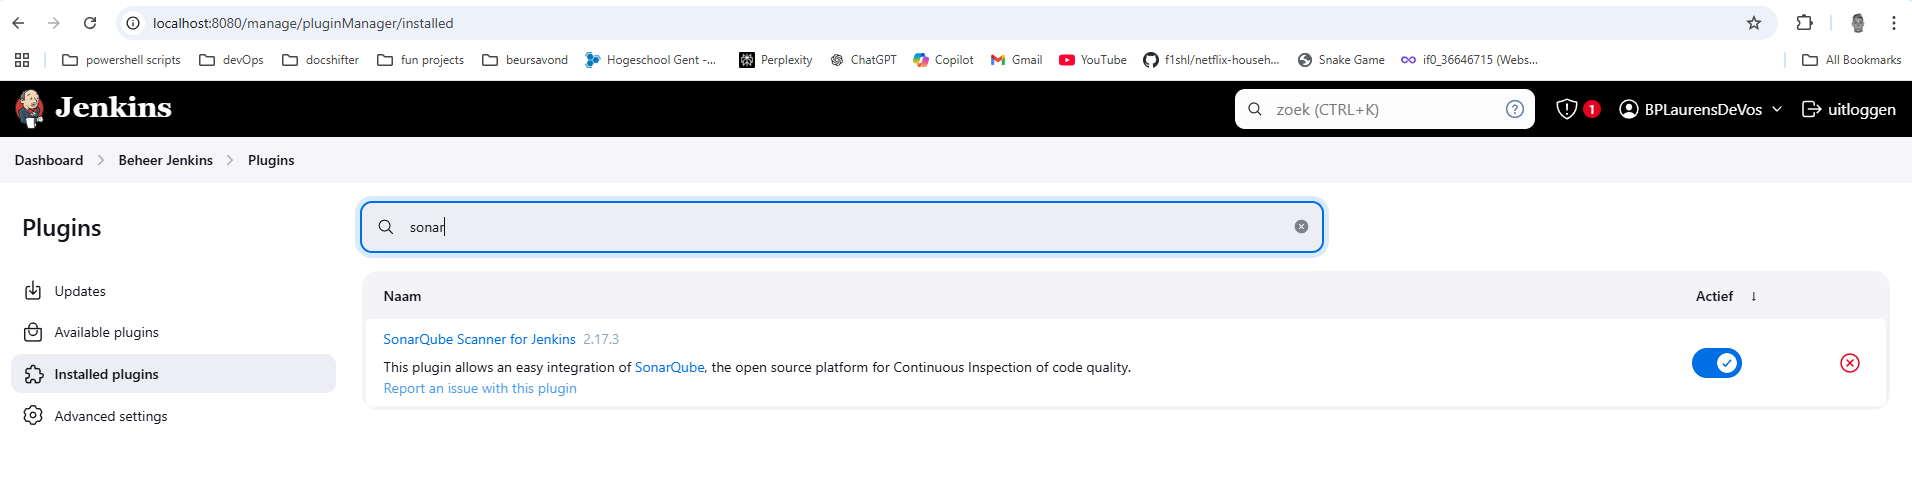
\includegraphics[width=\linewidth]{"C:/Users/laure/Documents/bachelorproef-2024-2025-laurensDeVos/graphics/SonarPlugin.png"}
    \caption{SonarQube scanner plugin geïnstalleerd op de Jenkins server}
    \label{fig:install_Sonar}
\end{figure}

\subsubsection{Configureren van Credentials}

Om de Jenkins-pipeline te laten werken, zijn credentials toegevoegd om toegang te geven tot GitHub en SonarCloud. Dit proces is vergelijkbaar met het configureren van GitHub Secrets in GitHub Actions. De configuratie werd uitgevoerd als volgt:

\begin{enumerate}
    \item \textbf{Toegang tot Credential Management}:
    Ga naar \texttt{Manage Jenkins > Credentials > System > Global Credentials}.
    \item \textbf{Toevoegen van credentials}:
    Voeg de volgende credentials toe als secret text:
    \begin{itemize}
        \item \textbf{GITHUB\_ACTOR}: GitHub-gebruikersnaam.
        \item \textbf{PAT\_TOKEN}: GitHub Personal Access Token, aangemaakt met de rechten \texttt{repo}, \texttt{read:packages}, en \texttt{write:packages}.
        \item \textbf{SONAR\_TOKEN}: Authenticatietoken voor SonarCloud, gegenereerd via \texttt{My Account > Security} in SonarCloud.
    \end{itemize}
    \item \textbf{Bevestiging van credentials}:
    Controleer of de credentials correct zijn opgeslagen. Het overzicht is beschikbaar in de \texttt{Global Credentials}-lijst.
\end{enumerate}

\begin{figure}[h!]
    \centering
    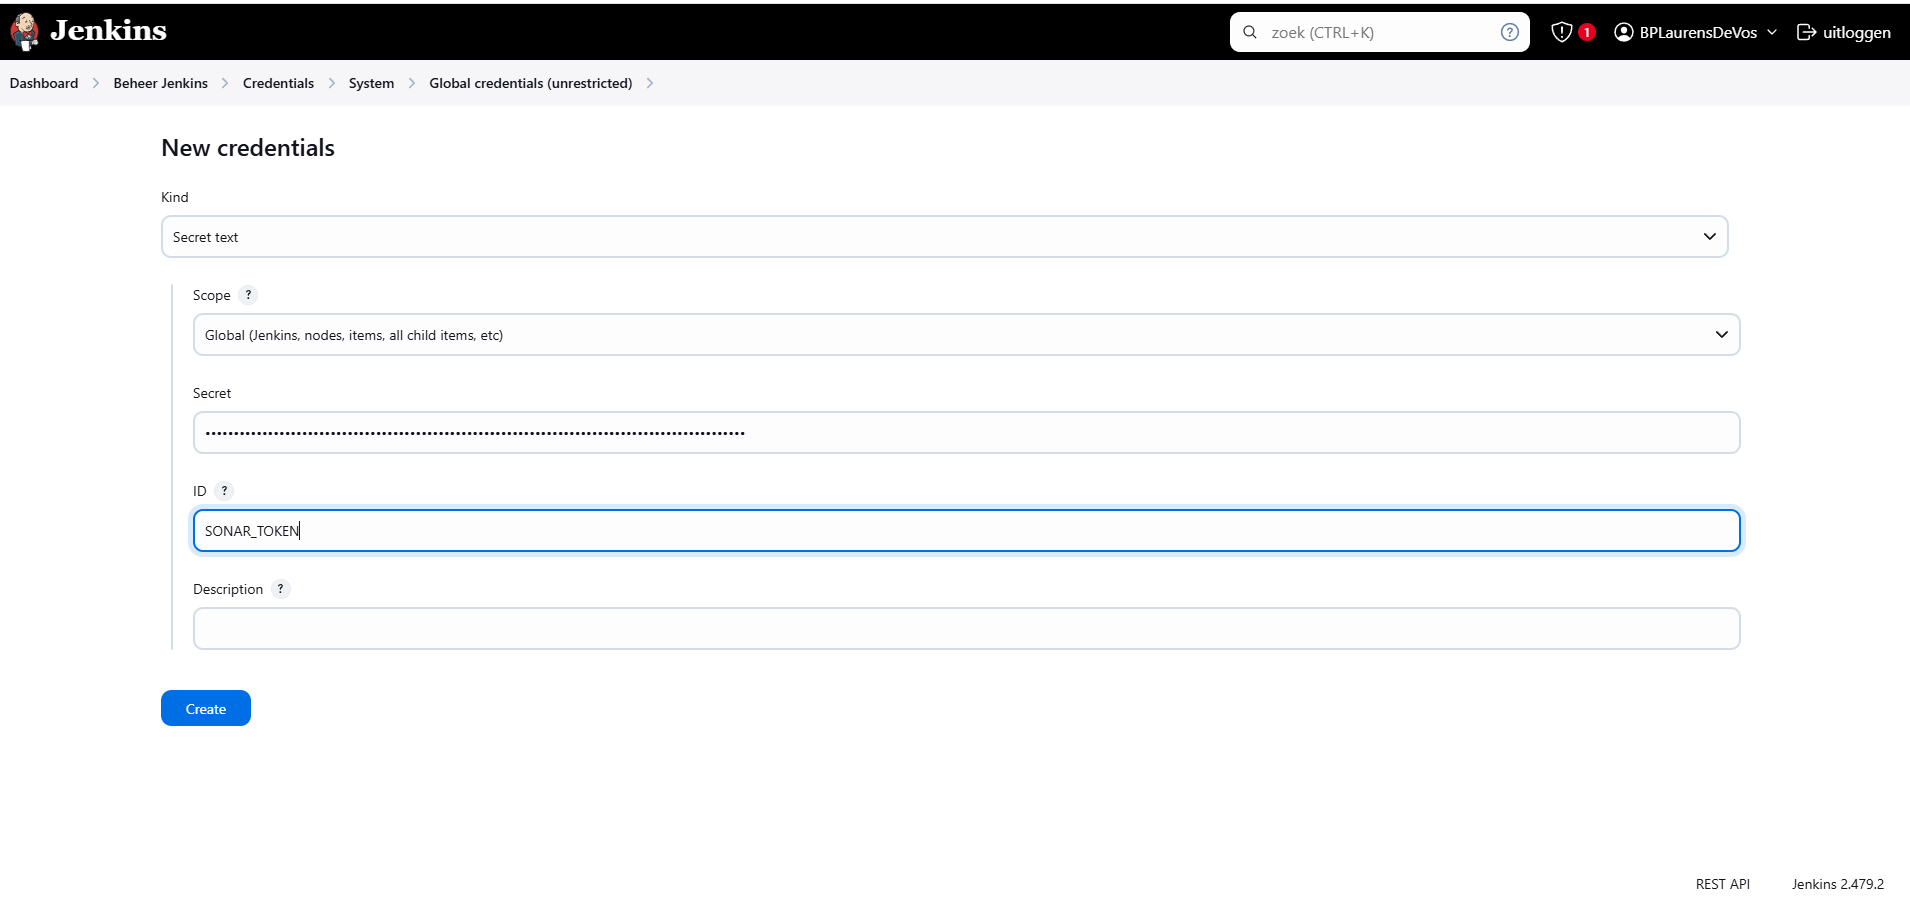
\includegraphics[width=\linewidth]{"C:/Users/laure/Documents/bachelorproef-2024-2025-laurensDeVos/graphics/addCredentials.png"}
    \caption{Toevoegen van credentials in Jenkins.}
    \label{fig:add_credentials}
\end{figure}

\begin{figure}[h!]
    \centering
    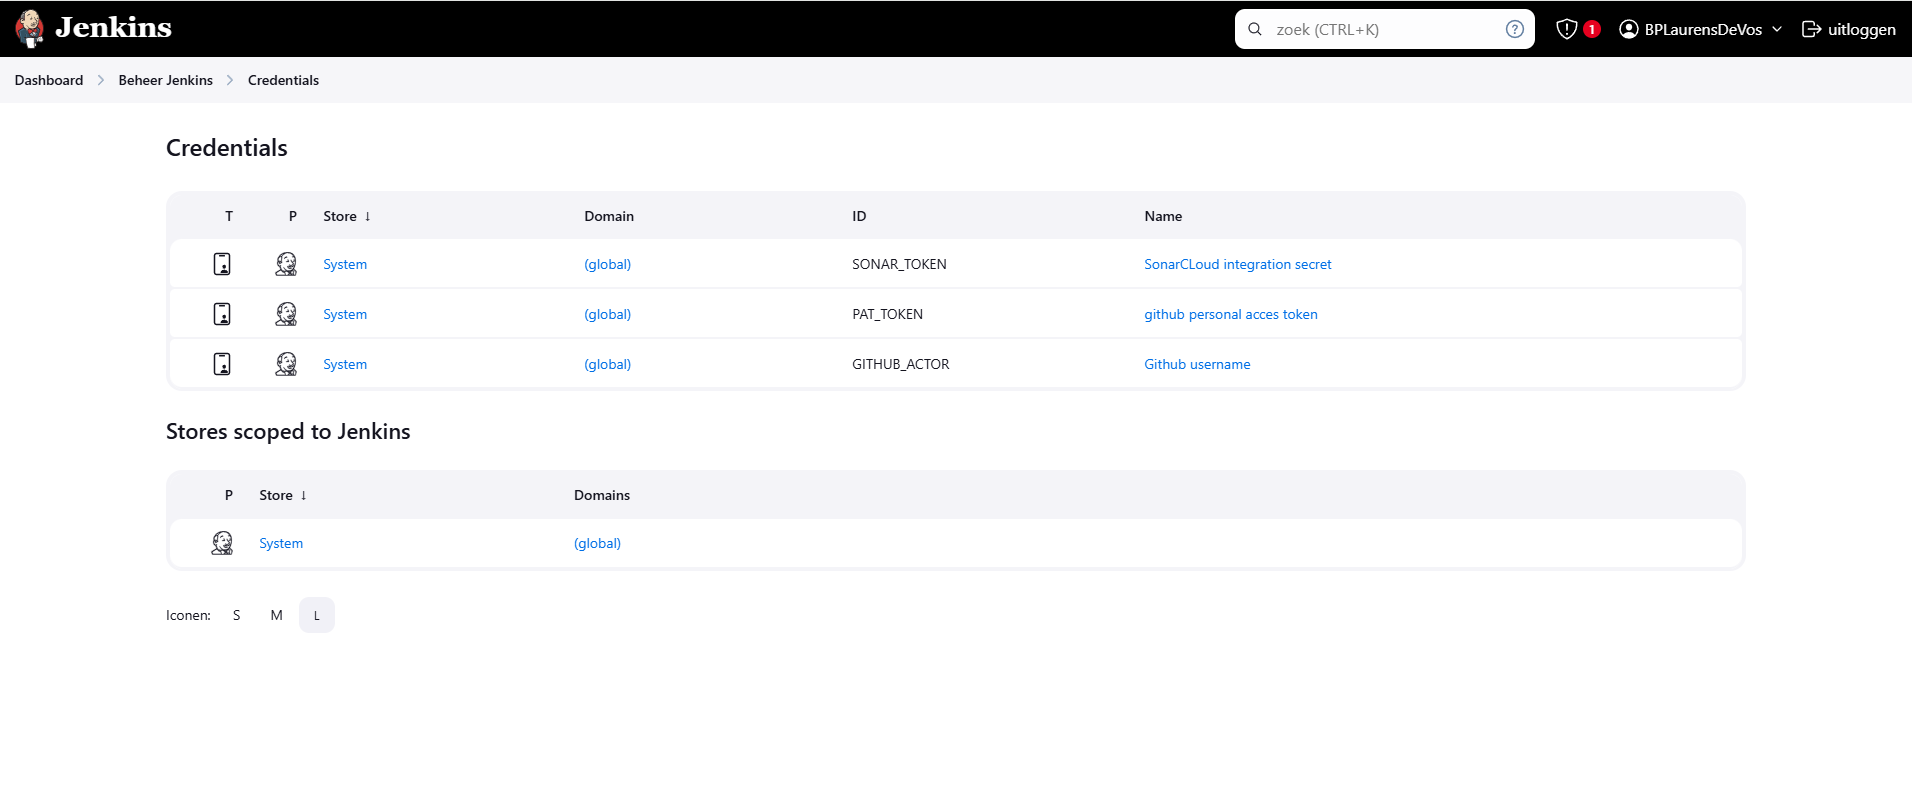
\includegraphics[width=\linewidth]{"C:/Users/laure/Documents/bachelorproef-2024-2025-laurensDeVos/graphics/overzichtCred.png"}
    \caption{Overzicht van geconfigureerde credentials in Jenkins.}
    \label{fig:overview_credentials}
\end{figure}

\subsubsection{Configuratie van de Jenkins Pipeline}

De configuratie van de Jenkins pipeline volgt een vergelijkbare aanpak als de implementatie in GitHub Actions. De Jenkinsfiles voor alle repositories (\texttt{Repo1} tot en met \texttt{Repo5}) zijn gebaseerd op een gestandaardiseerd formaat. Het doel is om een consistent CI/CD-proces te creëren dat kan worden vergeleken met de workflows in Actions.

\paragraph{Aanmaak van de Jenkins Pipeline}

Voor elk van de repositories is een Jenkins pipeline aangemaakt in de Jenkins webinterface. Hier zijn de stappen die zijn gevolgd:

\begin{enumerate} 
    \item Navigeer naar het Jenkins Dashboard:
    Open de Jenkins webinterface en klik op \texttt{New Item} in het dashboard.
    \item Geef een naam aan de pipeline:  
    Voer een unieke naam in voor de pipeline, bijvoorbeeld \texttt{Repo1}, en selecteer het itemtype \texttt{Pipeline}. Klik vervolgens op \texttt{OK}.
    
    \item Configureer de repository in de configuratiepagina:
    \begin{itemize}
        \item Navigeer naar de sectie \texttt{Pipeline}.
        \item Selecteer \texttt{Pipeline script from SCM} als de bron.
        \item Configureer de Git-repository-URL (bijvoorbeeld \texttt{https://github.com/BPLaurensDeVos/repo1}).
        \item Specificeer de branch (\texttt{main}) en het pad naar de Jenkinsfile (\texttt{Jenkinsfile}).
    \end{itemize}
    
    \item Klik op \texttt{Save} om de configuratie van de pipeline op te slaan.
\end{enumerate}   

\paragraph{Algemene structuur van de Jenkinsfile}
De Jenkinsfiles maken gebruik van declarative pipelines, waarin de stappen voor elke repository gedefinieerd zijn in afzonderlijke \texttt{stages}. De Jenkinsfiles worden gedefinieerd in de root map van de repository. De algemene structuur bestaat uit:
\begin{itemize}
    \item Het configureren van tools zoals Maven en JDK.
    \item Het ophalen van de broncode via Git.
    \item Het controleren van afhankelijkheden.
    \item Het bouwen, testen en publiceren van artefacten.
    \item Integratie met SonarCloud voor codekwaliteit.
\end{itemize}

\subparagraph{Tools configuratie}
\begin{verbatim}
        
        tools {
            maven 'Maven3'
            jdk 'jdk17'
        }
        

\end{verbatim}

\begin{itemize}
    \item \textbf{Maven}: Geeft aan dat Maven versie 3 wordt gebruikt als buildtool. Deze is vooraf geconfigureerd in Jenkins onder \texttt{Manage Jenkins > Global Tool Configuration}.
    \item \textbf{JDK}: Specificeert dat JDK versie 17 wordt gebruikt, wat compatibel is met de codebase van het project. Deze versie is nodig voor het compileren van de Java-code.
\end{itemize}

\begin{figure}[h!]
    \centering
    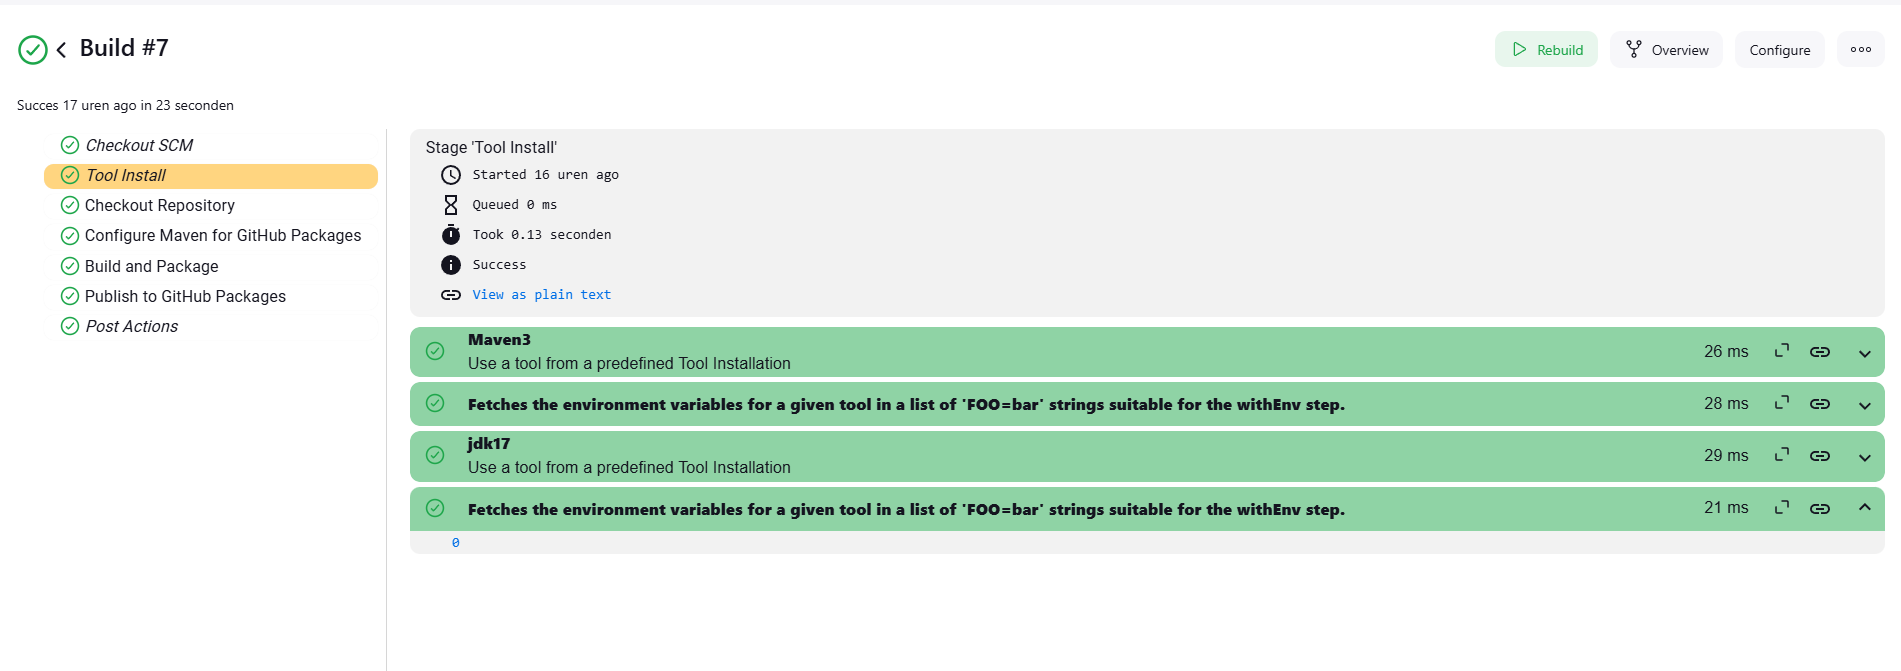
\includegraphics[width=\linewidth]{"C:/Users/laure/Documents/bachelorproef-2024-2025-laurensDeVos/graphics/toolInstall.png"}
    \caption{De uitvoer van de tool installatie in de pipeline.}
\end{figure}

\subparagraph{Environment configuratie}
\begin{verbatim}
    
        environment {
            GITHUB_ACTOR = credentials('GITHUB_ACTOR')
            GITHUB_TOKEN = credentials('PAT_TOKEN')
        }
  
\end{verbatim}

\begin{itemize}
    \item \textbf{GITHUB\_ACTOR}: Verwijst naar de GitHub-gebruikersnaam. Deze wordt opgeslagen als een credential in Jenkins onder \texttt{Manage Jenkins > Credentials}.
    \item \textbf{PAT\_TOKEN}: Dit is een Personal Access Token (PAT) dat wordt gebruikt voor authenticatie bij GitHub. Het token biedt toegang tot de repository en stelt Maven in staat om artefacten naar GitHub Packages te publiceren.
\end{itemize}

\subparagraph{Stages uitleg}
\textbf{Stage 1: Checkout Repository}
Deze stap zorgt voor het ophalen van de meest recente broncode van de repository door gebruik te maken van \textbf{checkout scm}.

\begin{verbatim}
    
    stage('Checkout Repository') {
        steps {
            echo "Checking out repository..."
            checkout scm
        }
    }

\end{verbatim}

\begin{figure}[h!]
    \centering
    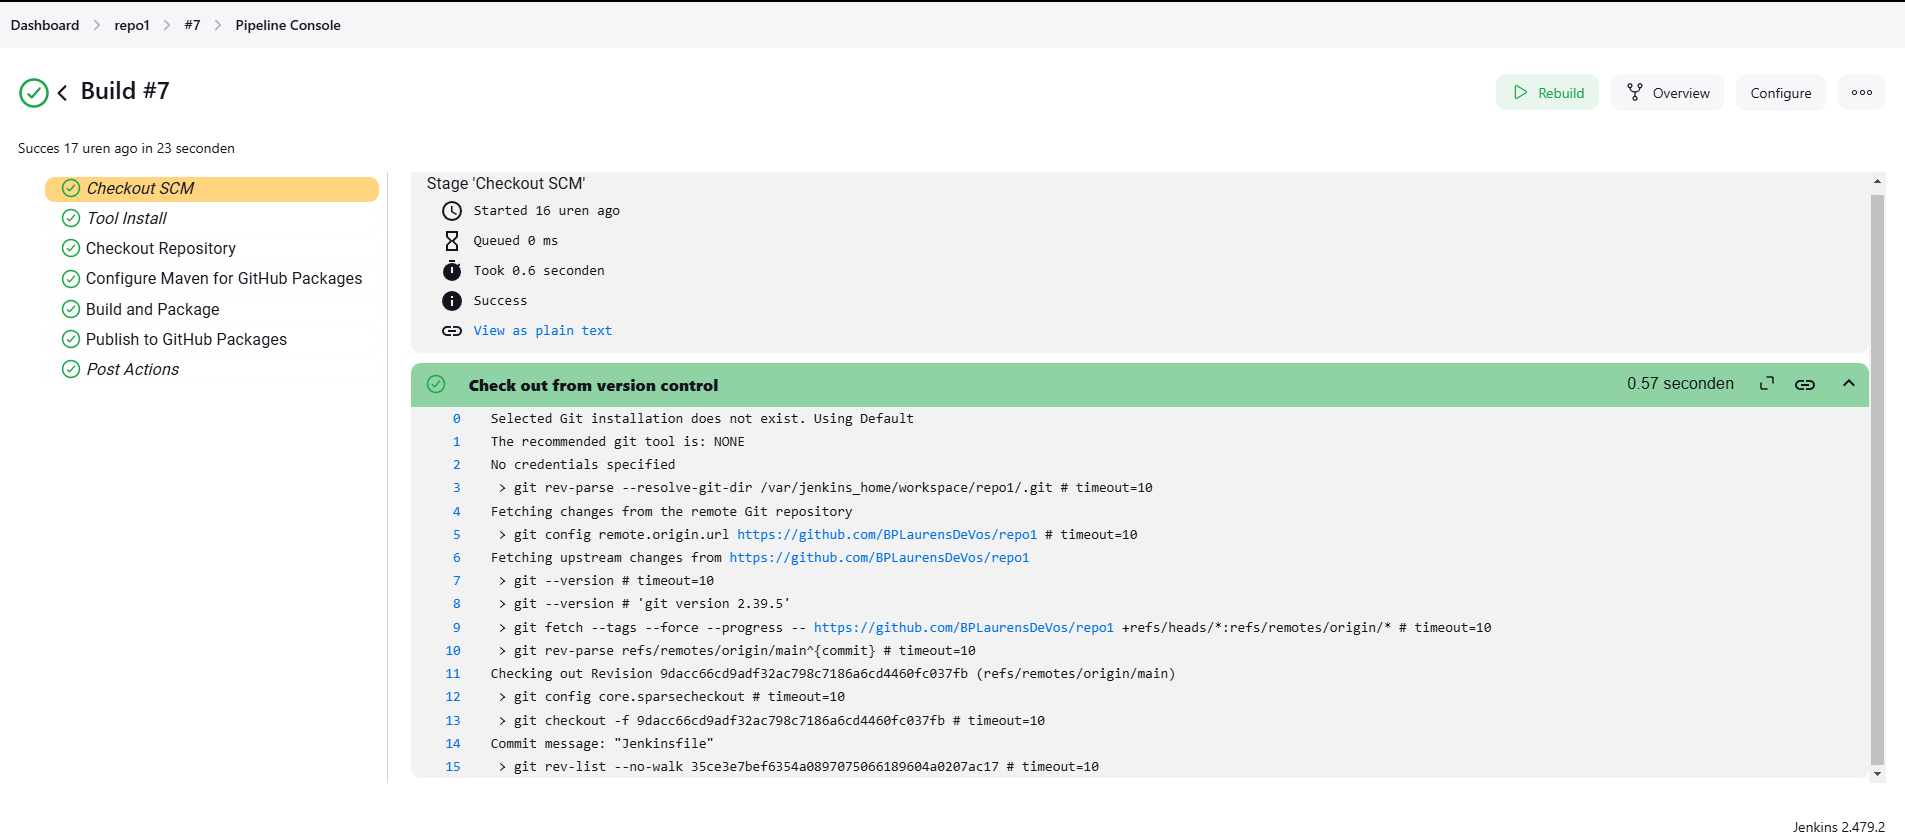
\includegraphics[width=\linewidth]{"C:/Users/laure/Documents/bachelorproef-2024-2025-laurensDeVos/graphics/checkoutscm.png"}
    \caption{De uitvoer tijdens het ophalen van de meest recente broncode van GitHub}
\end{figure}


\textbf{Stage 2: Configure Maven for GitHub Packages}
Deze stap zorgt voor het aanmaken van settings.xml die authenticatiegegevens bevat om toegang te krijgen tot Github Packages.

\begin{verbatim}
    
stage('Configure Maven for GitHub Packages') {
    steps {
        echo "Configuring Maven for GitHub Packages..."
        sh """
        mkdir -p ~/.m2
        echo "<settings xmlns='http://maven.apache.org/SETTINGS/1.0.0'>
            <servers>
              <server>
                <id>github</id>
                <username>${env.GITHUB_ACTOR}</username>
                <password>${env.GITHUB_TOKEN}</password>
              </server>
            </servers>
        </settings>" > ~/.m2/settings.xml
        """
    }
}
    
\end{verbatim}

\begin{figure}[h!]
    \centering
    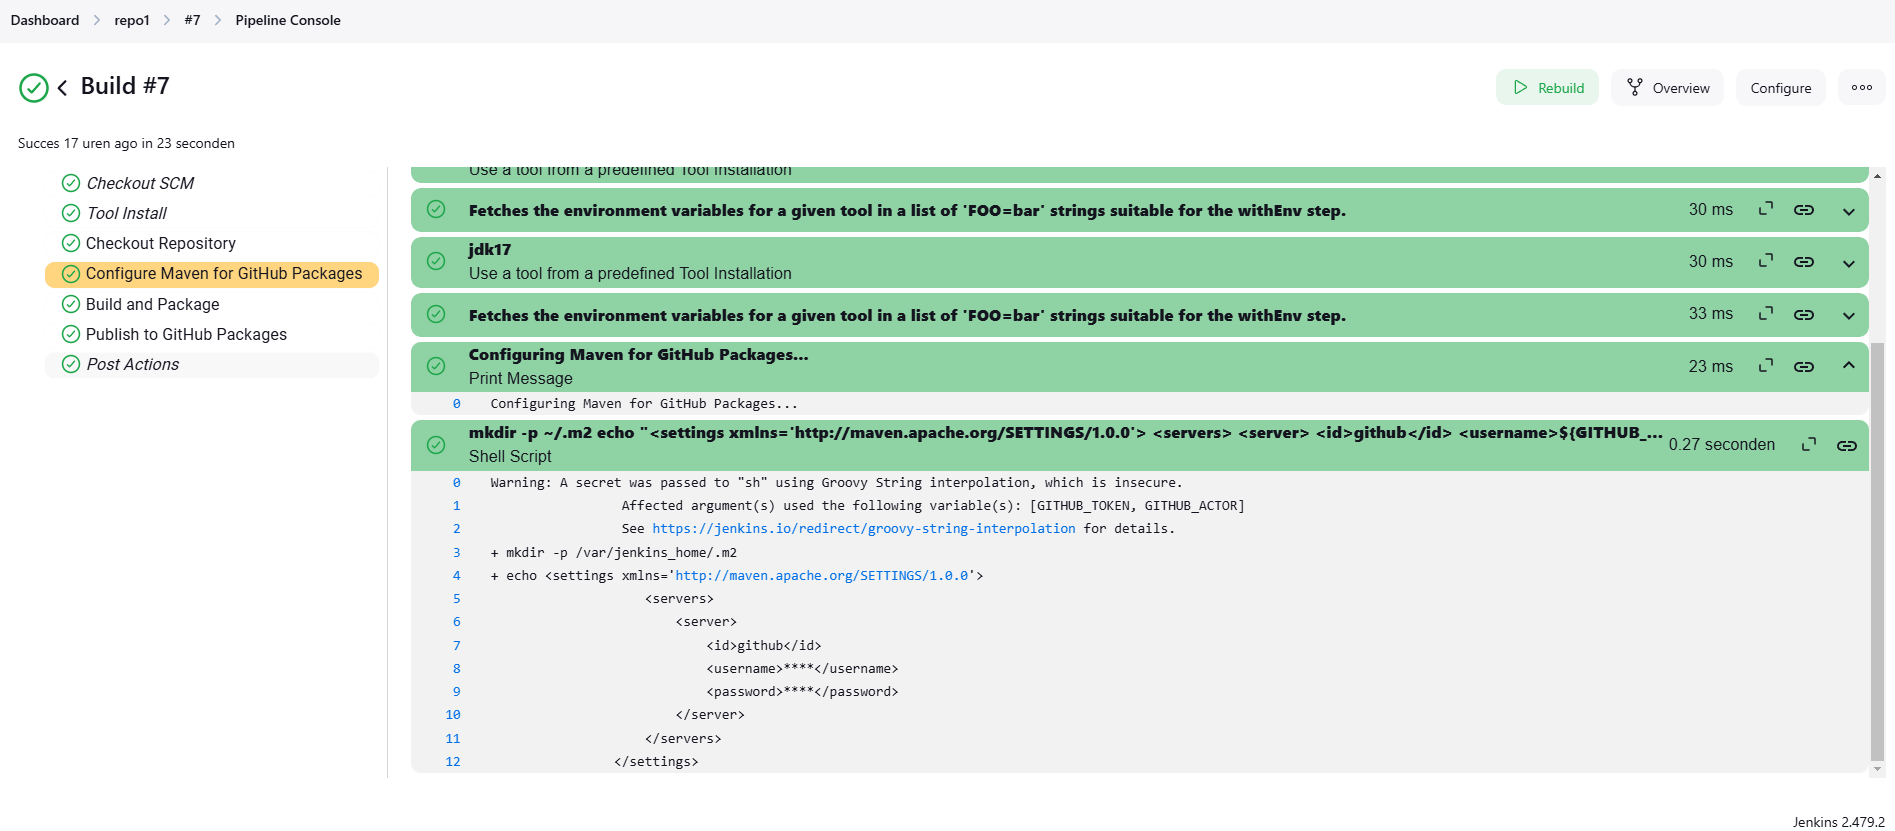
\includegraphics[width=\linewidth]{"C:/Users/laure/Documents/bachelorproef-2024-2025-laurensDeVos/graphics/confmvn.png"}
    \caption{De uitvoer van stage2.}
\end{figure}


\textbf{Stage 3: Build and Package}
Net zoals bij github actions wordt hetzelfde commando gebruikt om de java-code te compileren en testen.

\begin{verbatim}
    
    stage('Build and Package') {
        steps {
            echo "Building and packaging the project..."
            sh "mvn clean package"
        }
    }

    
\end{verbatim}

\begin{figure}[h!]
    \centering
    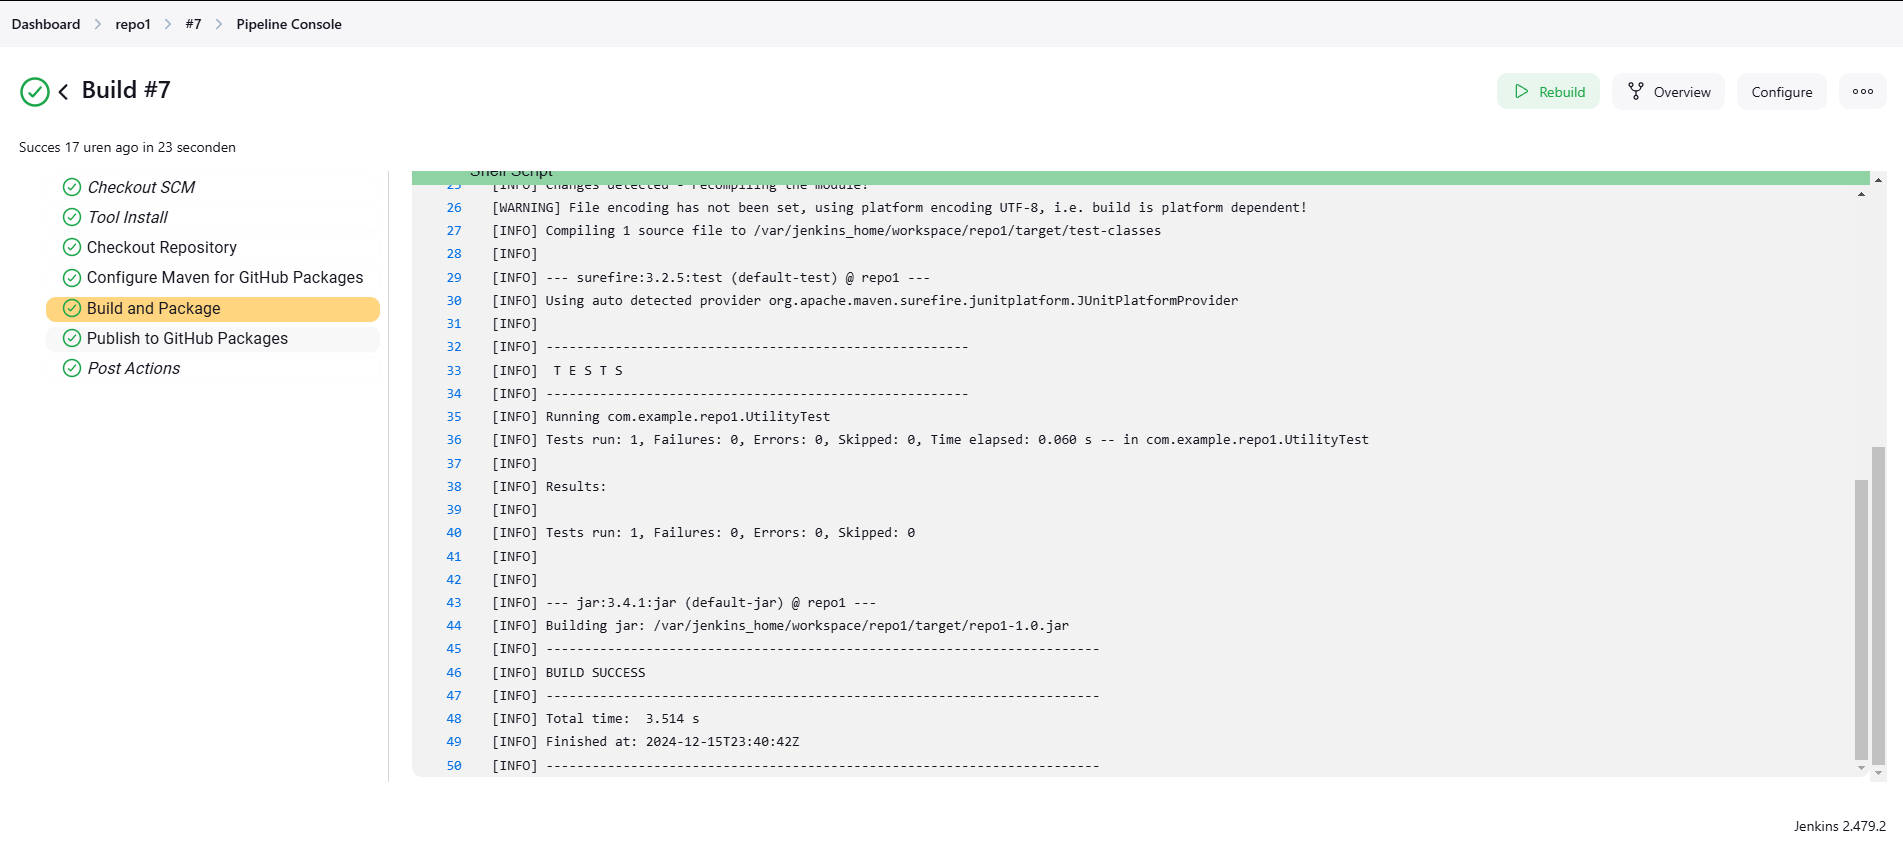
\includegraphics[width=\linewidth]{"C:/Users/laure/Documents/bachelorproef-2024-2025-laurensDeVos/graphics/buildpackagejenkins.png"}
    \caption{build succes toont aan dat de code is opgebouwd en getest.}
\end{figure}

\textbf{Stage 4: Publish to GitHub Packages}
Publiceert het gebouwde JAR-bestand van de vorige stage naar de GitHub Package Registry. 

\begin{verbatim}
    
    stage('Publish to GitHub Packages') {
        steps {
            echo "Publishing to GitHub Packages..."
            sh "mvn deploy"
        }
    }
    
\end{verbatim}

\begin{figure}[h!]
    \centering
    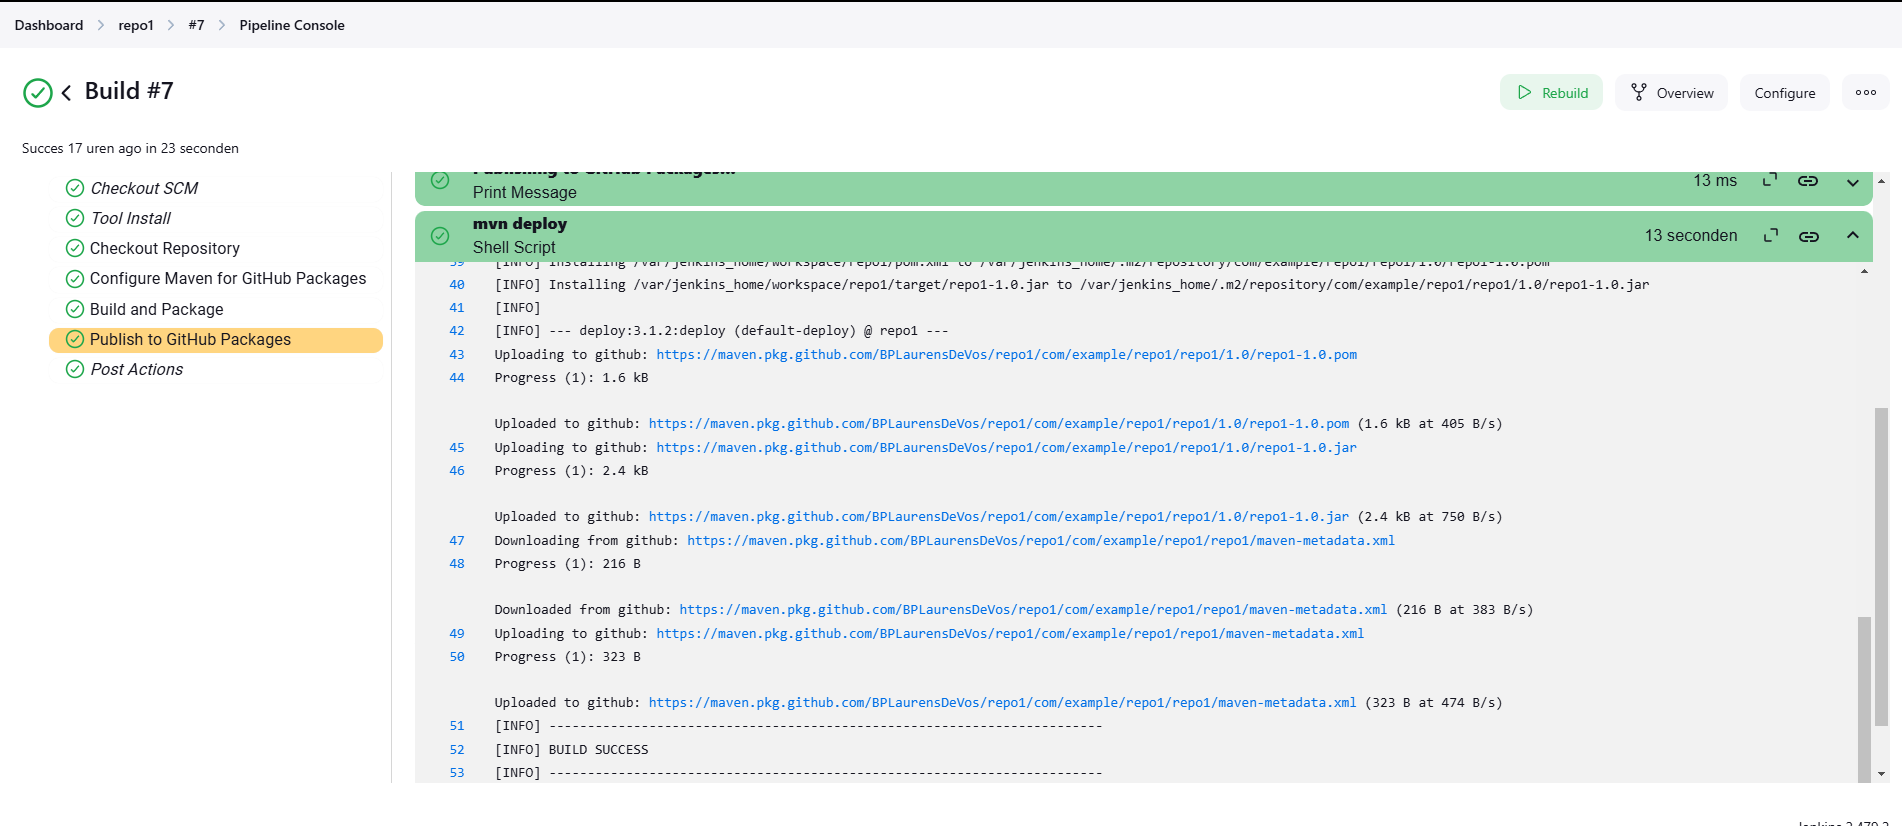
\includegraphics[width=\linewidth]{"C:/Users/laure/Documents/bachelorproef-2024-2025-laurensDeVos/graphics/publiceerjenkins.png"}
    \caption{Het artefact bestand wordt opgeladen in de GitHub Package Registry.}
\end{figure}

\subparagraph{Post-sectie uitleg}
Door deze code toe te voegen aan het bestand krijgen we feedback bij de uitvoering van de pipeline. 

\begin{verbatim}
    
    post {
        success {
            echo "Pipeline executed successfully for Repo1!"
        }
        failure {
            echo "Pipeline failed. Please check the logs for errors."
        }
    }

\end{verbatim}

\begin{figure}[h!]
    \centering
    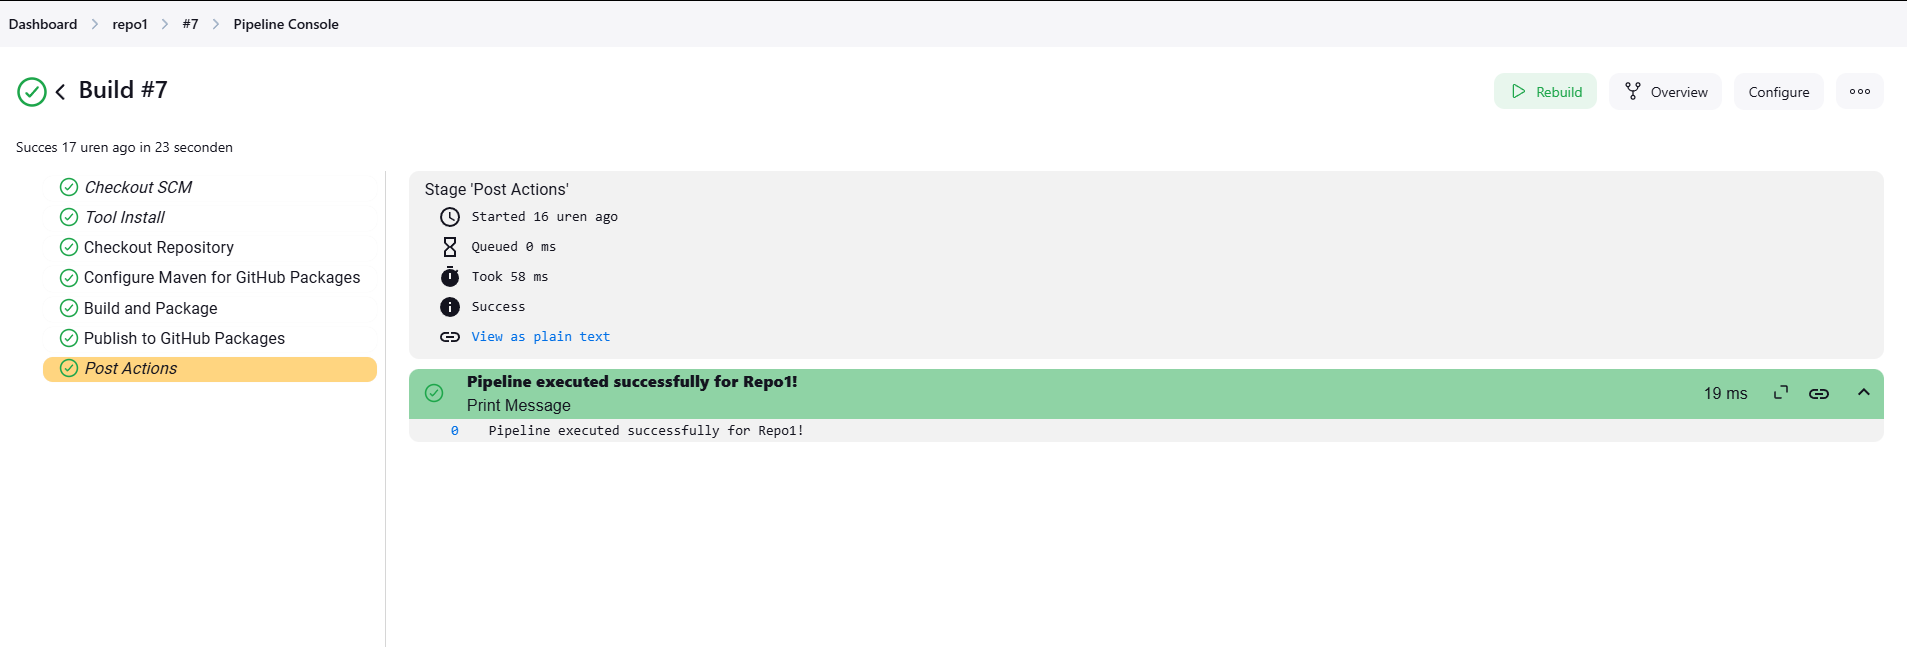
\includegraphics[width=\linewidth]{"C:/Users/laure/Documents/bachelorproef-2024-2025-laurensDeVos/graphics/post.png"}
    \caption{Een succesmelding wordt gegeven wanneer alle stages zonder fouten worden uitgevoerd.}
\end{figure}

\begin{figure}[h!]
    \centering
    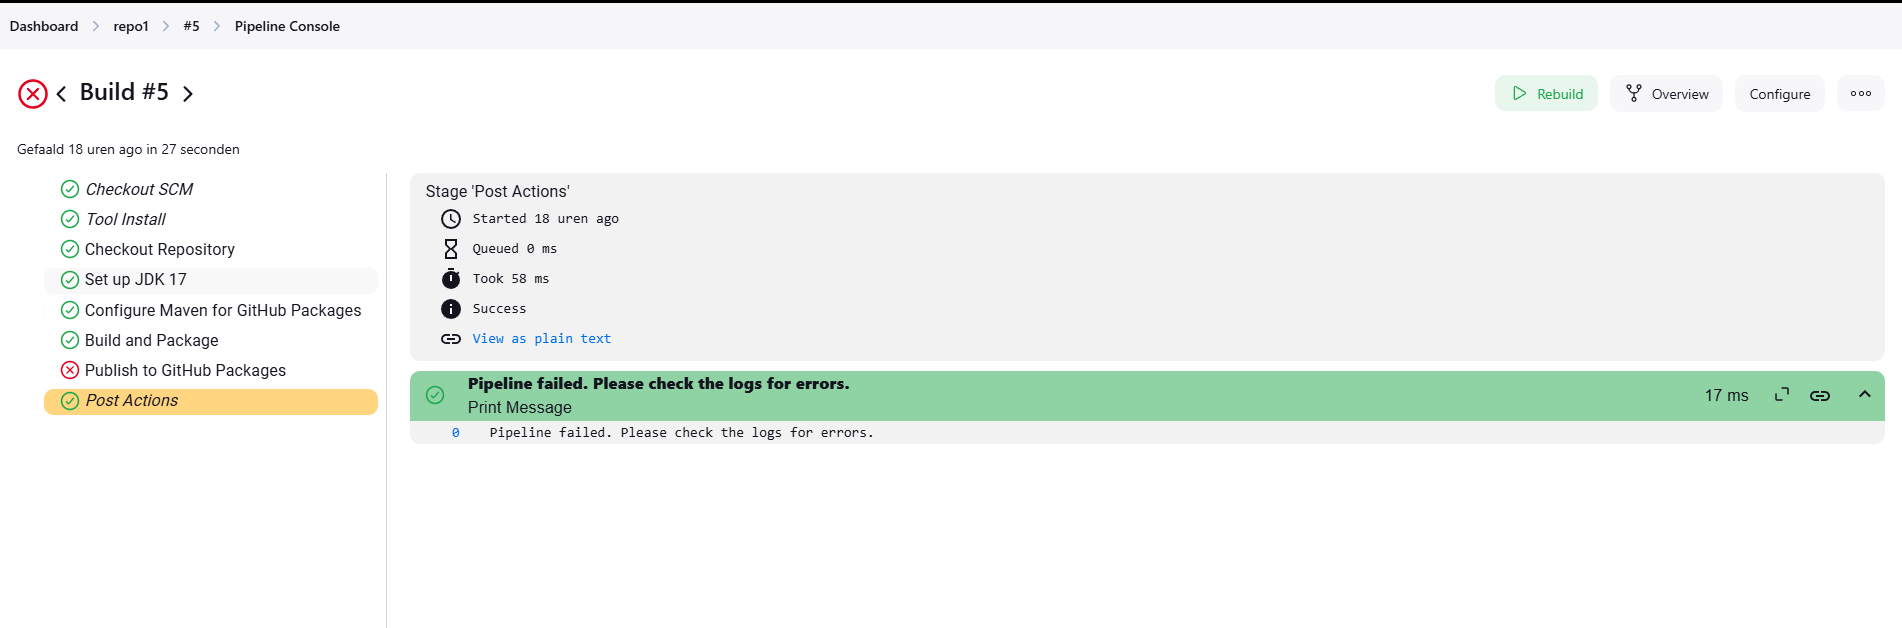
\includegraphics[width=\linewidth]{"C:/Users/laure/Documents/bachelorproef-2024-2025-laurensDeVos/graphics/postfout.png"}
    \caption{Een foutmelding wordt gegeven wanneer de pipeline een fout tegenkomt.}
\end{figure}

\subparagraph{Jenkinsfile voor repo1} 

\begin{verbatim}
    
    pipeline {
        agent any
        
        tools {
            maven 'Maven3'
            jdk 'jdk17'
        }
        
        environment {
            GITHUB_ACTOR = credentials('GITHUB_ACTOR')
            GITHUB_TOKEN = credentials('PAT_TOKEN')
        }
        
        stages {
            stage('Checkout Repository') {
                steps {
                    echo "Checking out repository..."
                    checkout scm
                }
            }
            
            stage('Configure Maven for GitHub Packages') {
                steps {
                    echo "Configuring Maven for GitHub Packages..."
                    sh """
                    mkdir -p ~/.m2
                    echo "<settings xmlns='http://maven.apache.org/SETTINGS/1.0.0'>
                        <servers>
                          <server>
                            <id>github</id>
                            <username>${env.GITHUB_ACTOR}</username>
                            <password>${env.GITHUB_TOKEN}</password>
                          </server>
                        </servers>
                    </settings>" > ~/.m2/settings.xml
                    """
                }
            }
            
            stage('Build and Package') {
                steps {
                    echo "Building and packaging the project..."
                    sh "mvn clean package"
                }
            }
            
            stage('Publish to GitHub Packages') {
                steps {
                    echo "Publishing to GitHub Packages..."
                    sh "mvn deploy"
                }
            }
        }
        
        post {
            success {
                echo "Pipeline executed successfully for Repo1!"
            }
            failure {
                echo "Pipeline failed. Please check the logs for errors."
            }
        }
    }

    
\end{verbatim}

\paragraph{Specifieke Configuraties voor downstream repositories}

\subparagraph{Configuratie voor \texttt{Repo2}}
Net zoals in GitHub Actions heeft \texttt{Repo2} een afhankelijkheid van \texttt{Repo1}. De pipeline voor \texttt{Repo2} controleert eerst of het artefact van \texttt{Repo1} beschikbaar is in GitHub Packages. Indien het artefact ontbreekt, wordt de Jenkins pipeline van \texttt{Repo1} getriggerd om het artefact te genereren. Vervolgens bouwt, test, en publiceert de pipeline het artefact van \texttt{Repo2}. 

Hieronder volgt een overzicht van de extra stappen in de Jenkinsfile voor repo2 tot en met repo5:

\begin{verbatim}
    stage('Artifact Check & Trigger') {
        steps {
            script {
                def statusCode = sh(
                script: "curl -L -u ${GITHUB_ACTOR}:${GITHUB_TOKEN} -s -o /dev/null -w '%{http_code}' ${REPO1_URL}",
                returnStdout: true
                ).trim()
                
                if (statusCode != '200') {
                    echo "Artifact missing. Triggering Repo1 Jenkins pipeline..."
                    build job: 'repo1', wait: true, propagate: true
                } else {
                    echo "Artifact is available. Proceeding with build."
                }
            }
        }
    }
\end{verbatim}

\textbf{Wat doet deze stap?}
\begin{itemize}
    \item Controleert de beschikbaarheid van het artefact van \texttt{repo1} met behulp van een HTTP-verzoek naar GitHub Packages.
    \item Start de Jenkins pipeline van \texttt{repo1} indien het artefact niet beschikbaar is met behulp van het \textbf{build job} commando.
\end{itemize}

\textbf{Waarom is deze stap belangrijk?}
\begin{itemize}
    \item Zorgt ervoor dat de afhankelijkheden correct worden beheerd en downstream builds niet falen vanwege ontbrekende artefacten.
    \item Dit mechanisme is essentieel voor het beheren van complexe afhankelijkheden tussen meerdere repositories.
\end{itemize}

Afbeelding \ref{fig:artifact_check_trigger} toont dat de pipeline in \texttt{Repo1} werd gestart door \texttt{Repo2}. Vervolgens werd \texttt{Repo2} getriggerd door \texttt{Repo3}, die op zijn beurt werd geactiveerd door \texttt{Repo4}, waarna het proces uiteindelijk begon bij \texttt{Repo5}.

\begin{figure}[h!]
    \centering
    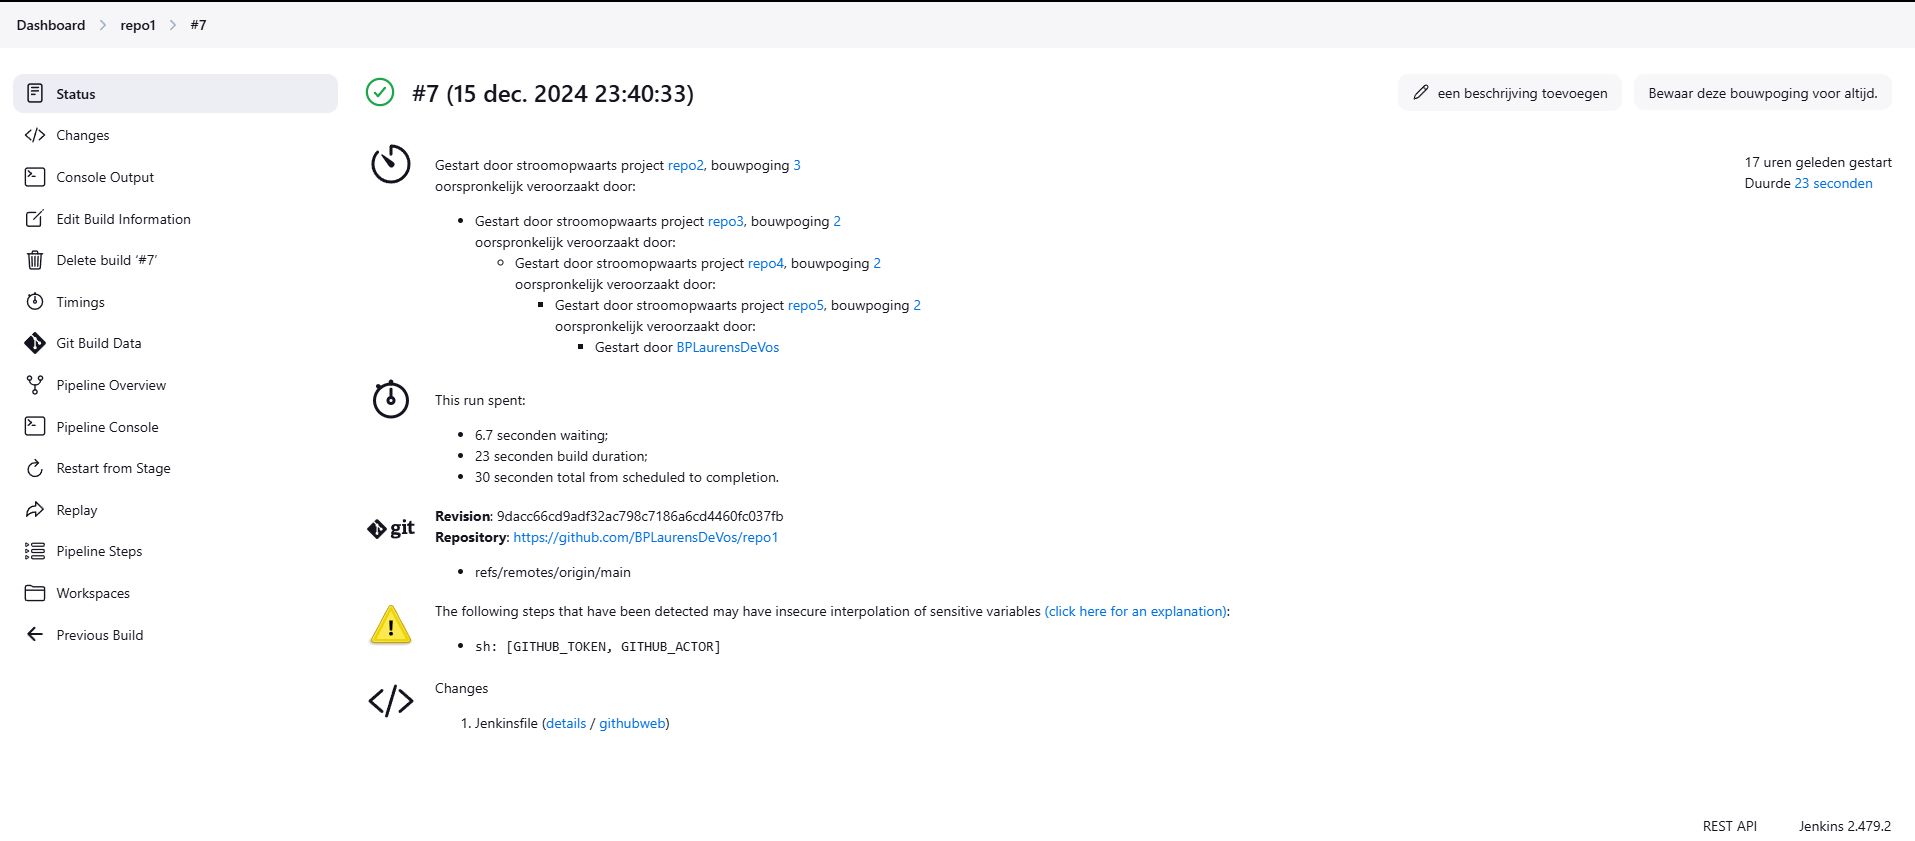
\includegraphics[width=\linewidth]{"C:/Users/laure/Documents/bachelorproef-2024-2025-laurensDeVos/graphics/triggerjenkins.png"}
    \label{fig:artifact_check_trigger}
\end{figure}

\subparagraph{Configuratie voor \texttt{Repo3}, \texttt{Repo4}, en \texttt{Repo5}}
De Jenkinsfiles voor \texttt{Repo3}, \texttt{Repo4}, en \texttt{Repo5} volgen dezelfde logica als \texttt{Repo2}, maar met aangepaste code voor afhankelijkheden. Zo controleert \texttt{Repo3} de beschikbaarheid van het artefact van \texttt{Repo2}.

Voorbeeld van de \texttt{Artifact Check} voor \texttt{Repo3}:

\begin{verbatim}
    stage('Artifact Check & Trigger') {
        steps {
            script {
                def statusCode = sh(
                script: "curl -L -u ${GITHUB_ACTOR}:${GITHUB_TOKEN} -s -o /dev/null -w '%{http_code}' ${REPO2_URL}",
                returnStdout: true
                ).trim()
                
                if (statusCode != '200') {
                    echo "Artifact missing. Triggering Repo2 Jenkins pipeline..."
                    build job: 'repo2', wait: true, propagate: true
                } else {
                    echo "Artifact is available. Proceeding with build."
                }
            }
        }
    }
\end{verbatim}

\paragraph{SonarCloud Integratie}
Net zoals in GitHub Actions wordt SonarCloud gebruikt om de codekwaliteit te bewaken. Dit gebeurt met de \texttt{SonarQube Scanner for Jenkins}-plugin. De configuratie is gedetailleerd beschreven in sectie \ref{subsec:voorbereidingvanhetproject} en wordt herhaald in de Jenkins pipeline met de volgende stap:

\begin{verbatim}
    stage('SonarCloud Scan') {
        steps {
            withSonarQubeEnv('SonarQube') {
                sh 'mvn sonar:sonar'
            }
        }
    }
\end{verbatim}

\textbf{Waarom belangrijk?}
\begin{itemize}
    \item Detecteert potentiële kwetsbaarheden in de code.
    \item Zorgt voor naleving van kwaliteitsstandaarden.
\end{itemize}

Afbeelding \ref{fig:sonarcloud_scan} toont de succesvolle uitvoering van een SonarCloud-scan in de omgeving op sonarcloud.

\begin{figure}[h!]
    \centering
    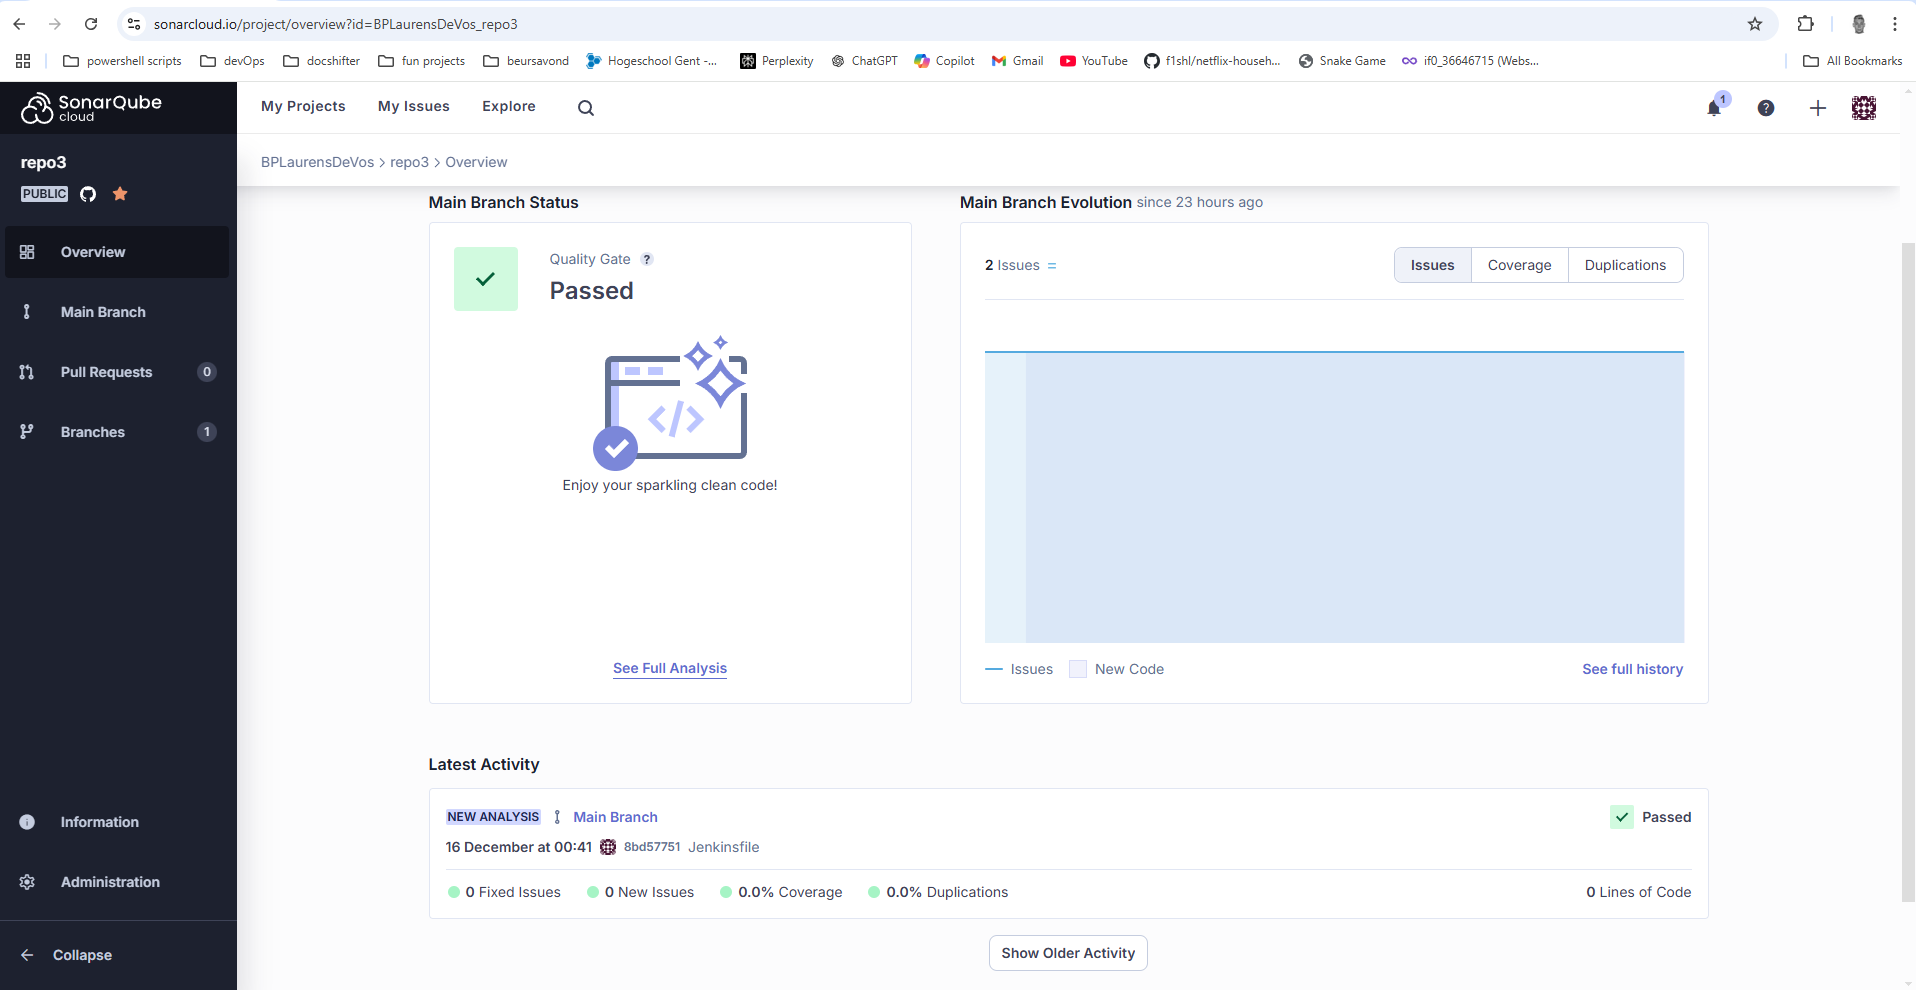
\includegraphics[width=\linewidth]{"C:/Users/laure/Documents/bachelorproef-2024-2025-laurensDeVos/graphics/sonarcloudjenkins.png"}
    \caption{Succesvolle SonarCloud scan opgestart door het Jenkinsfile.}
    \label{fig:sonarcloud_scan}
\end{figure}

\subparagraph{Jenkinsfile voor repo3} 

\begin{verbatim}
    
    pipeline {
        agent any
        
        tools {
            maven 'Maven3'
            jdk 'jdk17'
        }
        
        environment {
            GITHUB_ACTOR = credentials('GITHUB_ACTOR')
            GITHUB_TOKEN = credentials('PAT_TOKEN')
            SONAR_TOKEN = credentials('SONAR_TOKEN')
            REPO2_URL = "https://maven.pkg.github.com/BPLaurensDeVos/repo2/com/example/repo2/repo2/1.0/repo2-1.0.jar"
        }
        
        stages {
            stage('Checkout') {
                steps {
                    checkout scm
                }
            }
            
            stage('Artifact Check & Trigger') {
                steps {
                    script {
                        def statusCode = sh(
                        script: "curl -L -u ${GITHUB_ACTOR}:${GITHUB_TOKEN} -s -o /dev/null -w '%{http_code}' ${REPO2_URL}",
                        returnStdout: true
                        ).trim()
                        
                        if (statusCode != '200') {
                            echo "Artifact missing. Triggering Repo2 Jenkins pipeline..."
                            build job: 'repo2', wait: true, propagate: true
                        } else {
                            echo "Artifact is available. Proceeding with build."
                        }
                    }
                }
            }
            
            stage('Configure Maven') {
                steps {
                    sh """
                    mkdir -p ~/.m2
                    echo "<settings xmlns='http://maven.apache.org/SETTINGS/1.0.0'
                    xmlns:xsi='http://www.w3.org/2001/XMLSchema-instance'
                    xsi:schemaLocation='http://maven.apache.org/SETTINGS/1.0.0 https://maven.apache.org/xsd/settings-1.0.0.xsd'>
                    <servers>
                      <server>
                        <id>github-repo1</id>
                        <username>${GITHUB_ACTOR}</username>
                        <password>${GITHUB_TOKEN}</password>
                      </server>
                      <server>
                        <id>github-repo2</id>
                        <username>${GITHUB_ACTOR}</username>
                        <password>${GITHUB_TOKEN}</password>
                      </server>
                      <server>
                        <id>github-repo3</id>
                        <username>${GITHUB_ACTOR}</username>
                        <password>${GITHUB_TOKEN}</password>
                      </server>
                    </servers>
                    </settings>" > ~/.m2/settings.xml
                    """
                }
            }
            
            stage('Build and Test') {
                steps {
                    sh 'mvn clean package'
                }
            }
            
            stage('SonarCloud Scan') {
                steps {
                    withSonarQubeEnv('SonarCloud') {
                        sh 'mvn sonar:sonar'
                    }
                }
            }
            
            stage('Deploy to GitHub Packages') {
                steps {
                    sh 'mvn deploy'
                }
            }
        }
        
        post {
            success {
                echo 'Pipeline completed successfully.'
            }
            failure {
                echo 'Pipeline failed.'
            }
        }
    }

   
\end{verbatim}

\subparagraph{Conclusie}
De implementatie van CI/CD-pipelines met Jenkins biedt een flexibel en schaalbaar alternatief voor GitHub Actions. Dankzij het gebruik van Jenkinsfiles en het beheren van afhankelijkheden tussen repositories is een vergelijkbare workflow gecreëerd.


\section{Vergelijkende analyse van Jenkins en Github Actions}

\subsection{Inleiding}
In dit hoofdstuk worden Jenkins en GitHub Actions rechtstreeks met elkaar vergeleken op basis van de resultaten van de Proof-of-Concept (PoC). Door middel van deze analyse wordt beantwoord welke tool het meest geschikt is voor de specifieke behoeften van DocShifter, zoals aangegeven in de centrale onderzoeksvraag.

De vergelijking richt zich op vier kerncriteria:
\begin{itemize}
    \item \textbf{Prestaties}: Evaluatie van de snelheid en efficiëntie van builds in beide tools, met bijzondere aandacht voor eventuele bottlenecks.
    \item \textbf{Beveiliging}: Analyse van hoe beide tools omgaan met het beheer van credentials en toegangsrechten.
    \item \textbf{Automatiseringsefficiëntie}: Vergelijking van de eenvoud en flexibiliteit bij het configureren en beheren van workflows en pipelines.
    \item \textbf{Integratie met bestaande systemen}: Beoordeling van hoe gemakkelijk beide tools kunnen worden geïntegreerd met externe systemen en technologieën, zoals GitHub, Maven en SonarCloud.
\end{itemize}

Voor elk criterium worden de sterke en zwakke punten van Jenkins en GitHub Actions besproken, ondersteund door visuele weergaven zoals tabellen en grafieken. Het doel is om een objectieve en uitgebreide evaluatie te bieden die als basis kan dienen voor aanbevelingen.

\subsection{Vergelijkingscriteria}
Om de vergelijking systematisch en overzichtelijk te maken, zijn de volgende criteria gehanteerd:

\subsubsection{Prestaties}
Prestaties worden gemeten door de bouwtijden van Jenkins en GitHub Actions te vergelijken. Hierbij wordt specifiek gekeken naar:
\begin{itemize}
    \item \textbf{Buildduur}: Hoe lang duren de builds in beide tools, gemeten vanaf de start van een pipeline tot de succesvolle voltooiing.
    \item \textbf{Bottlenecks}: Zijn er vertragingen in de workflow? Bijvoorbeeld bij het verwerken van afhankelijkheden of bij het publiceren van artefacten.
\end{itemize}

\subsubsection{Beveiliging}
Bij beveiliging ligt de focus op hoe Jenkins en GitHub Actions omgaan met:
\begin{itemize}
    \item \textbf{Credentials}: Hoe worden credentials zoals GitHub-tokens en SonarCloud-tokens opgeslagen en beheerd?
\end{itemize}

\subsubsection{Automatiseringsefficiëntie}
Voor de automatiseringsefficiëntie wordt gekeken naar:
\begin{itemize}
    \item \textbf{Configuratiegemak}: Hoe eenvoudig is het om een pipeline of workflow op te zetten en te beheren?
    \item \textbf{Triggers}: Hoe effectief zijn de triggermechanismen, zoals \texttt{repository\_dispatch} in GitHub Actions en downstream jobs in Jenkins?
\end{itemize}

\subsubsection{Integratie met bestaande systemen}
Dit criterium onderzoekt hoe goed Jenkins en GitHub Actions kunnen worden geïntegreerd in de bestaande ontwikkelomgeving:
\begin{itemize}
    \item \textbf{Integratie met GitHub}: Hoe gemakkelijk kunnen beide tools worden gekoppeld aan repositories op GitHub?
    \item \textbf{Compatibiliteit met Java en Maven}: Hoe goed sluiten beide tools aan op de technologieën die worden gebruikt in de PoC, zoals Maven voor builds en SonarCloud voor codeanalyse?
\end{itemize}

\subsection{Vergelijking van Prestaties}

Een van de belangrijkste criteria bij het vergelijken van Jenkins en GitHub Actions is de \textbf{buildtijd} van de CI/CD-pipelines. De buildtijd bepaalt hoe snel een nieuwe versie van de applicatie kan worden gebouwd, getest en gedeployed, wat een cruciale factor is voor de efficiëntie van DevOps-processen.

\subsubsection{Buildtijden per repository}

Voor deze vergelijking werden \textbf{drie metingen} uitgevoerd voor elk van de vijf repositories (\texttt{Repo1} tot \texttt{Repo5}) in zowel Jenkins als GitHub Actions. De gemeten tijden zijn weergegeven in tabel~\ref{tab:performance_comparison}. De gemiddelde buildtijd werd berekend om een helder overzicht te geven.

\begin{table}[h!]
    \centering
    \caption{Vergelijking van buildtijden tussen Jenkins en GitHub Actions (in minuten en seconden)}
    \label{tab:performance_comparison}
    \begin{tabular}{|c|c|c|c|c|}
        \hline
        \textbf{Repository} & \textbf{Jenkins (s)} & \textbf{Gemiddelde} & \textbf{GitHub Actions (s)} & \textbf{Gemiddelde} \\
        \hline
        Repo1 & 28, 23, 24 & 25 & 29, 35, 31 & 31.7 \\
        Repo2 & 1:11, 1:19, 1:18 & 1:16 & 1:14, 1:09, 1:08 & 1:10 \\
        Repo3 & 2:02, 2:11, 2:11 & 2:08 & 2:30, 2:20, 2:59 & 2:29 \\
        Repo4 & 2:49, 3:04, 3:03 & 2:59 & 3:35, 3:44, 3:45 & 3:41 \\
        Repo5 & 3:36, 4:01, 3:57 & 3:51 & 4:38, 4:41, 4:45 & 4:41 \\
        \hline
    \end{tabular}
\end{table}

\paragraph{Analyse van de resultaten}
De resultaten laten duidelijk zien dat \textbf{Jenkins} over het algemeen snellere buildtijden behaalt in vergelijking met GitHub Actions. De verschillen worden groter naarmate de repositories meer afhankelijkheden hebben en de pipelines complexer worden (bijvoorbeeld bij \texttt{Repo3}, \texttt{Repo4}, en \texttt{Repo5}). Hieronder worden enkele opvallende observaties besproken:

\begin{itemize}
    \item \textbf{Repo1}: De buildtijd in Jenkins is gemiddeld 25 seconden, terwijl GitHub Actions gemiddeld 31,7 seconden nodig heeft. Dit verschil van enkele seconden kan worden toegeschreven aan een efficiëntere uitvoering van basistaken in Jenkins.
    
    \item \textbf{Repo2 tot Repo5}: In de complexere repositories wordt het verschil meer uitgesproken. In \texttt{Repo5} duurt de pipeline in Jenkins gemiddeld 3 minuten en 51 seconden, terwijl GitHub Actions hiervoor 4 minuten en 41 seconden nodig heeft. Dit verschil van bijna een minuut kan een significant voordeel bieden bij grotere projecten.
    
    \item \textbf{Toename in wachttijd bij GitHub Actions}: Een belangrijke factor die bijdraagt aan de langere buildtijden in GitHub Actions is het gebruik van de \texttt{sleep}-functie. Deze functie werd gebruikt om downstream pipelines (repositories) te laten wachten totdat upstream artefacten beschikbaar waren. In GitHub Actions moet de wachttijd statisch worden ingesteld, bijvoorbeeld 30 seconden of 90 seconden, afhankelijk van de repository. Dit kan leiden tot onnodige vertragingen wanneer de artefacten eerder klaar zijn.
    
    \item \textbf{Dynamic triggers in Jenkins}: In tegenstelling tot GitHub Actions, gebruikt Jenkins dynamische triggers. Wanneer een pipeline afhankelijk is van een upstream repository, wacht Jenkins automatisch tot de upstream build is voltooid voordat de downstream pipeline wordt gestart. Dit elimineert onnodige wachttijden en zorgt voor een efficiëntere uitvoering van afhankelijkheden.
\end{itemize}

\subsubsection{Bottlenecks in GitHub Actions}
Zoals eerder vermeld, is het gebruik van de \texttt{sleep}-functie in GitHub Actions een duidelijke bottleneck. Deze aanpak heeft twee nadelen:
\begin{enumerate}
    \item \textbf{Inefficiënt wachten}: Wanneer een upstream build sneller klaar is dan de ingestelde wachttijd, wordt er onnodig tijd verspild.
    \item \textbf{Hardcoded vertragingen}: De wachttijd moet handmatig worden ingesteld en kan variëren afhankelijk van de buildsnelheid, wat leidt tot inconsistenties.
\end{enumerate}

\subsubsection{Voordeel van Jenkins bij afhankelijkheden}
Jenkins biedt een efficiëntere oplossing voor het beheren van afhankelijkheden tussen repositories:
\begin{itemize}
    \item \textbf{Triggering van upstream jobs}: In Jenkins wacht de pipeline dynamisch totdat de afhankelijkheden gebouwd zijn. Dit gebeurt met behulp van de \texttt{build} opdracht in de pipeline:
    \begin{verbatim}
        build job: 'repo1', wait: true, propagate: true
    \end{verbatim}
    \item \textbf{Efficiënt gebruik van wachttijd}: Omdat Jenkins de afhankelijkheden automatisch beheert, worden downstream jobs direct gestart zodra de vereiste artefacten beschikbaar zijn. Dit vermindert de totale buildtijd aanzienlijk.
\end{itemize}

In de tabel \ref{tab:wait_time_comparison} wordt dit nog eens visueel verduidelijkt.

\begin{table}[h!]
    \centering
    \caption{Vergelijking van wachttijd en downstream builds in GitHub Actions en Jenkins.}
    \label{tab:wait_time_comparison}
    \begin{tabular}{|l|l|l|l|}
        \hline
        \textbf{CI/CD Tool}      & \textbf{Buildfase Repo2} & \textbf{Wachttijd (sleep)} & \textbf{Start Downstream Job}   \\ \hline
        \textbf{GitHub Actions}  & Build Repo2 loopt        & Start direct (sleep)       & Na wachttijd start Repo3        \\ \hline
        \textbf{Jenkins}         & Build Repo2 voltooit     & Geen                       & Repo3 start zodra Repo2 klaar is \\ \hline
    \end{tabular}
\end{table}


\subsubsection{Conclusie over prestaties}
Op basis van de gemeten buildtijden en de observaties kunnen we concluderen dat:
\begin{itemize}
    \item \textbf{Jenkins} efficiënter omgaat met afhankelijkheden dankzij dynamische triggers, wat leidt tot kortere buildtijden, vooral in complexe pipelines.
    \item \textbf{GitHub Actions} ervaart vertragingen door het gebruik van statische wachttijden (\texttt{sleep}), wat resulteert in langere totale buildtijden.
\end{itemize}

Voor projecten met meerdere afhankelijkheden en complexe workflows biedt Jenkins een prestatievoordeel, terwijl GitHub Actions eenvoudiger kan zijn voor kleinere, minder afhankelijke projecten.

\subsubsection{Vergelijking van beveiliging}

In dit onderdeel wordt het beheer en de bescherming van credentials in Jenkins en GitHub Actions besproken. Beide tools bieden ingebouwde functies om gevoelige informatie zoals tokens en gebruikersnamen te beheren. De analyse richt zich op twee aspecten: hoe credentials worden beheerd en of ze zichtbaar zijn in de uitvoeringslogboeken.

\paragraph{Credentials Management in Jenkins}

Jenkins maakt gebruik van een Credential Store om gevoelige informatie veilig te beheren. In deze Proof-of-Concept (PoC) werden de volgende credentials ingesteld:
\begin{itemize}
    \item \textbf{GITHUB\_ACTOR}: GitHub-gebruikersnaam.
    \item \textbf{PAT\_TOKEN}: Personal Access Token voor authenticatie bij GitHub.
    \item \textbf{SONAR\_TOKEN}: Authenticatietoken voor SonarCloud.
\end{itemize}

\textbf{Toevoeging van credentials}  
Credentials werden toegevoegd via het Jenkins Dashboard onder \texttt{Manage Jenkins > Credentials}. Hier werden ze geconfigureerd als globale secrets die toegankelijk zijn voor alle pipelines.

\textbf{Voorbeeld van gebruik in Jenkinsfile:}
\begin{verbatim}
    environment {
        GITHUB_ACTOR = credentials('GITHUB_ACTOR')
        GITHUB_TOKEN = credentials('PAT_TOKEN')
    }
\end{verbatim}

\textbf{Bescherming van credentials}  
Jenkins maskert credentials standaard in de uitvoeringslogboeken. Zoals te zien in de console output, worden de waarden van \texttt{GITHUB\_ACTOR} en \texttt{GITHUB\_TOKEN} vervangen door \texttt{****} wanneer ze worden gebruikt in een shell-script. Dit voorkomt dat gevoelige informatie zichtbaar wordt.

\textbf{Voorbeeld uit de console output:}
\begin{verbatim}
    Warning: A secret was passed to "sh" using Groovy String interpolation, which is insecure.
                Affected argument(s) used the following variable(s): [GITHUB_TOKEN, GITHUB_ACTOR]
                See https://jenkins.io/redirect/groovy-string-interpolation for details.
    + mkdir -p /var/jenkins_home/.m2
    + echo <settings xmlns='http://maven.apache.org/SETTINGS/1.0.0'>
                <servers>
                  <server>
                    <id>github</id>
                    <username>****</username>
                    <password>****</password>
                  </server>
                </servers>
            </settings>
\end{verbatim}

\textbf{Waarschuwing voor onveilige praktijken}  
Jenkins detecteert potentieel onveilige praktijken, zoals het gebruik van credentials in shell-scripts via stringinterpolatie. Deze waarschuwing benadrukt dat er verbeteringen mogelijk zijn in de implementatie van de pipelines. Dit aspect kan worden verbeterd door gebruik te maken van veilige methoden zoals Jenkins-pipelinemodules voor credentialbeheer.

Een overzicht van geconfigureerde credentials was eerder al te zien in afbeelding \ref{fig:overview_credentials}.


\paragraph{Credentials Management in GitHub Actions}

GitHub Actions biedt een geïntegreerd systeem voor het beheren van secrets via het tabblad \texttt{Settings > Secrets and variables > Actions}. In deze Proof-of-Concept (PoC) werden de volgende secrets gebruikt:
\begin{itemize}
    \item \textbf{PAT\_TOKEN}: Personal Access Token voor authenticatie bij GitHub.
    \item \textbf{SONAR\_TOKEN}: Authenticatietoken voor SonarCloud.
\end{itemize}

\textbf{Toevoeging van secrets}  
Secrets worden toegevoegd aan de repository-instellingen. Deze zijn toegankelijk voor workflows via omgevingsvariabelen. Het gebruik van secrets in workflows wordt hieronder geïllustreerd:

\textbf{Voorbeeld in workflow:}
\begin{verbatim}
    env:
    GITHUB_ACTOR: ${{ github.actor }}
    GITHUB_TOKEN: ${{ secrets.PAT_TOKEN }}
\end{verbatim}

\textbf{Bescherming van credentials}  
GitHub Actions maskeert standaard de waarden van secrets in de uitvoerlogboeken door ze te vervangen door \texttt{***}. Echter, de gebruikersnaam \texttt{GITHUB\_ACTOR}, die niet als secret wordt behandeld, blijft zichtbaar in de logs. 

Er bestaan methoden om ook gebruikersnamen te maskeren in GitHub Actions:
\begin{itemize}
    \item Door de gebruikersnaam als een secret op te slaan en deze in plaats van \texttt{GITHUB\_ACTOR} te gebruiken.
    \item Door het commando \texttt{::add-mask::} te gebruiken, waarmee specifieke strings handmatig in de logs kunnen worden gemaskeerd.
\end{itemize}

Voor deze PoC is bewust gekozen om de gebruikersnaam zichtbaar te laten. De redenen hiervoor zijn:
\begin{itemize}
    \item Transparantie en eenvoud bij het debuggen van workflows.
    \item De gebruikte accounts bevatten geen gevoelige informatie en zijn specifiek aangemaakt voor CI/CD-doeleinden.
\end{itemize}

Afbeelding~\ref{fig:github_logs_actor} toont een voorbeeld waarin de gebruikersnaam zichtbaar blijft in de logs, terwijl de waarde van \texttt{PAT\_TOKEN} correct wordt gemaskeerd.

\begin{figure}[h!]
    \centering
    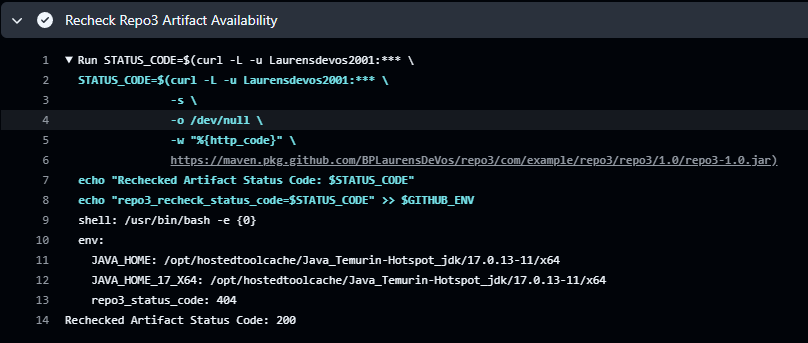
\includegraphics[width=\linewidth]{"C:/Users/laure/Documents/bachelorproef-2024-2025-laurensDeVos/graphics/mask.png"}
    \caption{Voorbeeld van logs in GitHub Actions waarin de gebruikersnaam zichtbaar is en tokens zijn gemaskeerd.}
    \label{fig:github_logs_actor}
\end{figure}

\paragraph{Vergelijking tussen Jenkins en GitHub Actions}
In de tabel \ref{tab:credentials_comparison} is een overzichtelijke vergelijking te zien tussen Jenkins en GitHub Actions.

\begin{table}[h!]
    \centering
    \begin{tabular}{|p{4cm}|p{5cm}|p{5cm}|}
        \hline
        \textbf{Aspect}               & \textbf{Jenkins}                                                                                                 & \textbf{GitHub Actions}                                                                                        \\ \hline
        \textbf{Beheer van credentials} & Credentials worden centraal beheerd in de Credential Store.                                                & Secrets worden beheerd op repositoryniveau via de instellingen van GitHub.                               \\ \hline
        \textbf{Bescherming in logboeken} & Credentials worden standaard gemaskeerd (\texttt{****}).                                                       & Secrets (\texttt{PAT\_TOKEN}) worden gemaskeerd, en gebruikersnamen kunnen optioneel worden gemaskeerd met extra configuratie. \\ \hline
        \textbf{Waarschuwingen}         & Geeft waarschuwingen voor onveilige praktijken zoals Groovy String interpolatie.                          & Geen waarschuwingen voor het gebruik van secrets in workflows, maar biedt een optie om gebruikersnamen te maskeren. \\ \hline
        \textbf{Flexibiliteit}          & Brede ondersteuning voor verschillende typen credentials (secret text, SSH-sleutels, certificaten, etc.). & Ondersteuning voor repository-, organisatie-, en omgevingsniveau secrets.                                                                 \\ \hline
    \end{tabular}
    \caption{Vergelijking van credentials management tussen Jenkins en GitHub Actions.}
    \label{tab:credentials_comparison}
\end{table}

\paragraph{Conclusie}

Jenkins biedt een robuust credentials management systeem met standaard masking en waarschuwingen voor onveilige praktijken. GitHub Actions biedt eenvoudiger integratie met GitHub, maar vereist extra configuratie om gebruikersnamen zoals \texttt{GITHUB\_ACTOR} te maskeren. Voor deze PoC is bewust gekozen om gebruikersnamen zichtbaar te laten in GitHub Actions, gezien het gebruik van dedicated CI/CD-accounts en de voordelen voor transparantie en debugging.

\subsubsection{Vergelijking op automatiseringsefficiëntie}

In deze sectie wordt de automatiseringsefficiëntie van Jenkins en GitHub Actions vergeleken. Hierbij wordt gekeken naar het configuratiegemak, het instellen van triggers en de algemene gebruikservaring.

\paragraph{Configuratiegemak}

De webinterfaces van zowel Jenkins als GitHub Actions bieden een gebruiksvriendelijke ervaring. Echter, er zijn enkele verschillen in het configuratieproces:
\begin{itemize}
    \item \textbf{Jenkins:} Het opzetten van een basispipeline in Jenkins vereist meer stappen. Gebruikers moeten eerst een pipeline-item aanmaken in de webinterface voordat ze kunnen beginnen met het schrijven van een Jenkinsfile. Daarnaast vereist Jenkins de installatie en configuratie van de tool zelf (in dit geval via Docker) en het installeren van aanvullende plug-ins, zoals Maven en SonarQube-integratie.
    
    \item \textbf{GitHub Actions:} In GitHub Actions kan direct een workflowbestand worden aangemaakt in de repository. Dit bespaart tijd omdat er geen extra configuratie in een aparte webinterface nodig is. Bovendien zijn er geen plug-ins die handmatig geïnstalleerd moeten worden, omdat GitHub Actions direct geïntegreerd is met GitHub en populaire acties zoals \texttt{actions/checkout} beschikbaar stelt.
\end{itemize}

Het schrijven van pipeline-code zelf verschilt ook tussen de tools:
\begin{itemize}
    \item \textbf{Jenkinsfiles:} Het schrijven van Jenkinsfiles wordt als intuïtiever ervaren vanwege de duidelijke en gestructureerde syntax. Dit maakt het eenvoudiger om complexe pipelines te configureren.
    \item \textbf{GitHub Actions files:} Hoewel GitHub Actions YAML-bestanden overzichtelijk zijn, kunnen ze complex worden wanneer meerdere afhankelijkheden en geavanceerde configuraties nodig zijn.
\end{itemize}

\paragraph{Triggers}

Het instellen van triggers voor pipeline- of workflowuitvoering toont belangrijke verschillen tussen de twee tools:
\begin{itemize}
    \item \textbf{Jenkins:} Jenkins biedt een intuïtieve manier om downstream jobs te configureren, waardoor pipelines automatisch worden getriggerd op basis van afhankelijke repositories. Deze functionaliteit is eenvoudig te configureren via de Jenkins-webinterface of direct in de Jenkinsfile.
    
    \item \textbf{GitHub Actions:} Het configureren van triggers met \texttt{repository\_dispatch} werkt beperkt, omdat de communicatie slechts in één richting plaatsvindt. Daarnaast is het noodzakelijk om een wachttijd (\texttt{sleep}) toe te voegen om te voorkomen dat downstream workflows falen vanwege ontbrekende artefacten. Dit maakt het beheer van afhankelijkheden complexer en minder efficiënt in GitHub Actions.
\end{itemize}

Afbeelding \ref{fig:jenkins_trigger} toont de configuratie van triggers in Jenkins, terwijl afbeelding \ref{fig:github_dispatch} een voorbeeld illustreert van het gebruik van \texttt{repository\_dispatch} in GitHub Actions.

\begin{figure}[h!]
    \centering
    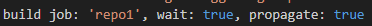
\includegraphics[width=\linewidth]{"C:/Users/laure/Documents/bachelorproef-2024-2025-laurensDeVos/graphics/jenkinstrigger.png"}
    \caption{Configuratie van downstream triggers in Jenkins.}
    \label{fig:jenkins_trigger}
\end{figure}

\begin{figure}[h!]
    \centering
    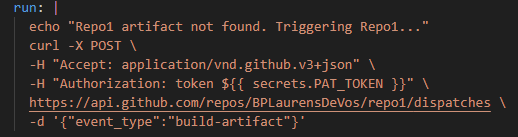
\includegraphics[width=\linewidth]{"C:/Users/laure/Documents/bachelorproef-2024-2025-laurensDeVos/graphics/actionstrigger.png"}
    \caption{Gebruik van \texttt{repository\_dispatch} in GitHub Actions.}
    \label{fig:github_dispatch}
\end{figure}

\paragraph{Conclusie}

Op het gebied van automatiseringsefficiëntie heeft GitHub Actions een voordeel in het snelle opzetten van eenvoudige workflows. Er is geen extra installatie of configuratie nodig, en workflows kunnen direct in GitHub worden beheerd. Voor meer complexe pipelines biedt Jenkins echter een robuustere oplossing, met betere ondersteuning voor triggers en afhankelijkheden tussen repositories. Dit maakt Jenkins geschikter voor scenario's met meerdere afhankelijkheden, zoals deze PoC.

\subsubsection{Integratie met bestaande systemen}
Dit onderdeel beoordeelt hoe goed Jenkins en GitHub Actions integreren met bestaande ontwikkelomgevingen en technologieën. Hierbij wordt specifiek gekeken naar de integratie met GitHub, Java, Maven en SonarCloud, zoals gebruikt in de Proof-of-Concept (PoC).

\paragraph{Integratie met GitHub}
\textbf{GitHub Actions} biedt een naadloze integratie met GitHub, aangezien het direct is ingebouwd in het platform. Workflows kunnen eenvoudig worden geactiveerd door gebeurtenissen zoals commits, pull requests of geplande taken. Dit maakt het opzetten van CI/CD-processen met GitHub Actions eenvoudig en intuïtief, zonder dat aanvullende configuraties nodig zijn.

In \textbf{Jenkins} vereist de integratie met GitHub meer configuratiestappen. De Git Plugin moet worden geïnstalleerd en geconfigureerd, waarna repositories handmatig moeten worden gekoppeld. Hoewel dit proces meer tijd kost, biedt het flexibiliteit door ondersteuning van meerdere versiebeheersystemen, niet beperkt tot GitHub.

\paragraph{Compatibiliteit met Java en Maven}
Beide tools bieden uitstekende ondersteuning voor Java en Maven. 
In de PoC zijn de volgende functionaliteiten geanalyseerd:
\begin{itemize}
    \item \textbf{GitHub Actions} gebruikt vooraf geconfigureerde acties uit de Marketplace, zoals \texttt{actions/setup-java}, voor het eenvoudig instellen van de juiste Java-versie en Maven-configuratie. Dit vereenvoudigt het proces aanzienlijk, met minimale handmatige configuratie.
    \item \textbf{Jenkins} maakt gebruik van de ingebouwde toolconfiguratie en plugins zoals de \texttt{Maven Integration Plugin}. Hoewel dit flexibiliteit biedt, vereist het meer handmatige configuratie, zoals het definiëren van tools en het instellen van specifieke versies.
\end{itemize}

\paragraph{Integratie met SonarCloud}
Voor kwaliteitscontrole en code-analyse is in de PoC SonarCloud geïntegreerd. 
\begin{itemize}
    \item In \textbf{GitHub Actions} is de integratie uitgevoerd met een officiële SonarCloud Action uit de Marketplace. Dit vereiste minimale configuratie en stelde de workflows in staat om naadloos analyses uit te voeren.
    \item In \textbf{Jenkins} werd de integratie bereikt door de installatie van de SonarQube Scanner Plugin. Dit proces vereist meer configuratiestappen, inclusief het handmatig instellen van de server-URL en authenticatietokens.
\end{itemize}

\paragraph{Conclusie}
GitHub Actions onderscheidt zich door zijn eenvoud en naadloze integratie met GitHub en andere ontwikkeltools, wat vooral voordelig is voor teams die volledig in het GitHub-ecosysteem werken. Jenkins biedt daarentegen meer flexibiliteit en kan beter worden aangepast aan complexe workflows of alternatieve versiebeheersystemen. Voor organisaties zoals DocShifter, die gebruik maken van Java en Maven, bieden beide tools voldoende ondersteuning. Echter, GitHub Actions kan worden aanbevolen voor snel op te zetten workflows, terwijl Jenkins geschikt is voor meer geavanceerde en op maat gemaakte integraties.

\begin{table}[h!]
    \centering
    \begin{tabular}{|p{5cm}|p{5cm}|p{5cm}|}
        \hline
        \textbf{Aspect} & \textbf{GitHub Actions} & \textbf{Jenkins} \\ \hline
        Integratie met GitHub & Naadloze ingebouwde integratie & Vereist handmatige configuratie met plugins \\ \hline
        Configuratie voor Java en Maven & Eenvoudig via Marketplace-acties & Flexibel, maar vereist meer handmatige configuratie \\ \hline
        Integratie met SonarCloud & Officiële actie beschikbaar in Marketplace & Vereist installatie en configuratie van plugins \\ \hline
    \end{tabular}
    \caption{Vergelijking van integratiekenmerken tussen GitHub Actions en Jenkins.}
    \label{tab:integration_comparison}
\end{table}




% Voeg hier je eigen hoofdstukken toe die de ``corpus'' van je bachelorproef
% vormen. De structuur en titels hangen af van je eigen onderzoek. Je kan bv.
% elke fase in je onderzoek in een apart hoofdstuk bespreken.

%\input{...}
%\input{...}
%...

%%=============================================================================
%% Conclusie
%%=============================================================================

\chapter{Conclusie}
\label{ch:conclusie}

De centrale onderzoeksvraag van deze bachelorproef was: 
\emph{“Welke Continuous Integration/Continuous Deployment (CI/CD)-tool, Jenkins of GitHub Actions, biedt de meest geschikte oplossing voor het verbeteren van de DevOps-processen van DocShifter in termen van prestaties, beveiliging, automatiseringsefficiëntie en integratie met bestaande systemen?”} 

Op basis van een uitgebreide literatuurstudie en de implementatie van een Proof-of-Concept (PoC) kan gesteld worden dat beide tools unieke voordelen en beperkingen hebben, afhankelijk van de specifieke behoeften van een organisatie.

\paragraph{Antwoord op de onderzoeksvraag}
De evaluatie heeft aangetoond dat:
\begin{itemize}
    \item \textbf{Jenkins} zich onderscheidt door zijn flexibiliteit en schaalbaarheid, dankzij uitgebreide plugin-ondersteuning en het vermogen om complexe afhankelijkheden tussen repositories te beheren. Dit maakt het een robuuste keuze voor organisaties met complexe workflows zoals DocShifter.
    \item \textbf{GitHub Actions} blinkt uit in gebruiksgemak en naadloze integratie binnen het GitHub-ecosysteem. De eenvoud van configuratie en de cloud-gebaseerde schaalbaarheid maken het een aantrekkelijke optie voor kleinere of minder complexe projecten.
\end{itemize}

Voor DocShifter, dat afhankelijk is van een netwerk van onderling afhankelijke repositories en een schaalbare infrastructuur vereist, biedt Jenkins de meest geschikte oplossing. De mogelijkheid om agents dynamisch in te richten en geavanceerde afhankelijkheidsbeheermechanismen te gebruiken, sluit goed aan bij de behoeften van het bedrijf.

\paragraph{Relevantie van de resultaten}
De resultaten van dit onderzoek zijn relevant voor organisaties die voor de uitdaging staan om een CI/CD-tool te kiezen die zowel technische als operationele eisen ondersteunt. De vergelijkende analyse biedt praktische inzichten die bijdragen aan een weloverwogen keuze en kan dienen als referentie voor toekomstige evaluaties van CI/CD-tools.

\paragraph{Reflectie en discussie}
Hoewel de resultaten grotendeels overeenkomen met de verwachtingen, zijn er enkele aandachtspunten die verdere studie verdienen:
\begin{itemize}
    \item \textbf{Beveiliging}: Hoewel beide tools robuuste beveiligingsmechanismen bieden, zoals secrets management, is een meer gedetailleerde vergelijking nodig van hun naleving van industrienormen zoals ISO 27001.
    \item \textbf{Kosten}: Een diepgaand kostenoverzicht, inclusief licenties, infrastructuurkosten en onderhoud, kan aanvullende inzichten bieden.
    \item \textbf{Automatiseringsefficiëntie}: De beperkingen van GitHub Actions met betrekking tot afhankelijkheidsbeheer zouden verder kunnen worden onderzocht, met name door third-party oplossingen of custom workflows.
\end{itemize}

\paragraph{Bijdrage aan het vakgebied}
Deze bachelorproef biedt een gestructureerde methodologie voor de evaluatie van CI/CD-tools en demonstreert hoe theoretische inzichten kunnen worden vertaald naar praktische toepassingen. De Proof-of-Concept vormt een nuttige referentie voor organisaties die vergelijkbare evaluaties willen uitvoeren.

\paragraph{Aanbevelingen voor toekomstig onderzoek}
Op basis van deze studie kunnen de volgende richtingen voor toekomstig onderzoek worden voorgesteld:
\begin{itemize}
    \item Onderzoek naar de prestaties van Jenkins en GitHub Actions in cloud-native omgevingen, zoals Kubernetes-gebaseerde infrastructuren.
    \item Analyse van de impact van geavanceerde beveiligingsintegraties (bijvoorbeeld DevSecOps) in beide tools.
    \item Vergelijking van CI/CD-tools in termen van ondersteuning voor andere programmeertalen en frameworks buiten Java en Maven.
\end{itemize}

Deze aanbevelingen bieden een waardevolle basis voor verdere optimalisatie van DevOps-processen in een steeds evoluerend technologisch landschap.




%---------- Bijlagen -----------------------------------------------------------

\appendix

\section{Appendix A: Workflow Resultaten}

\begin{figure}[h!]
    \centering
    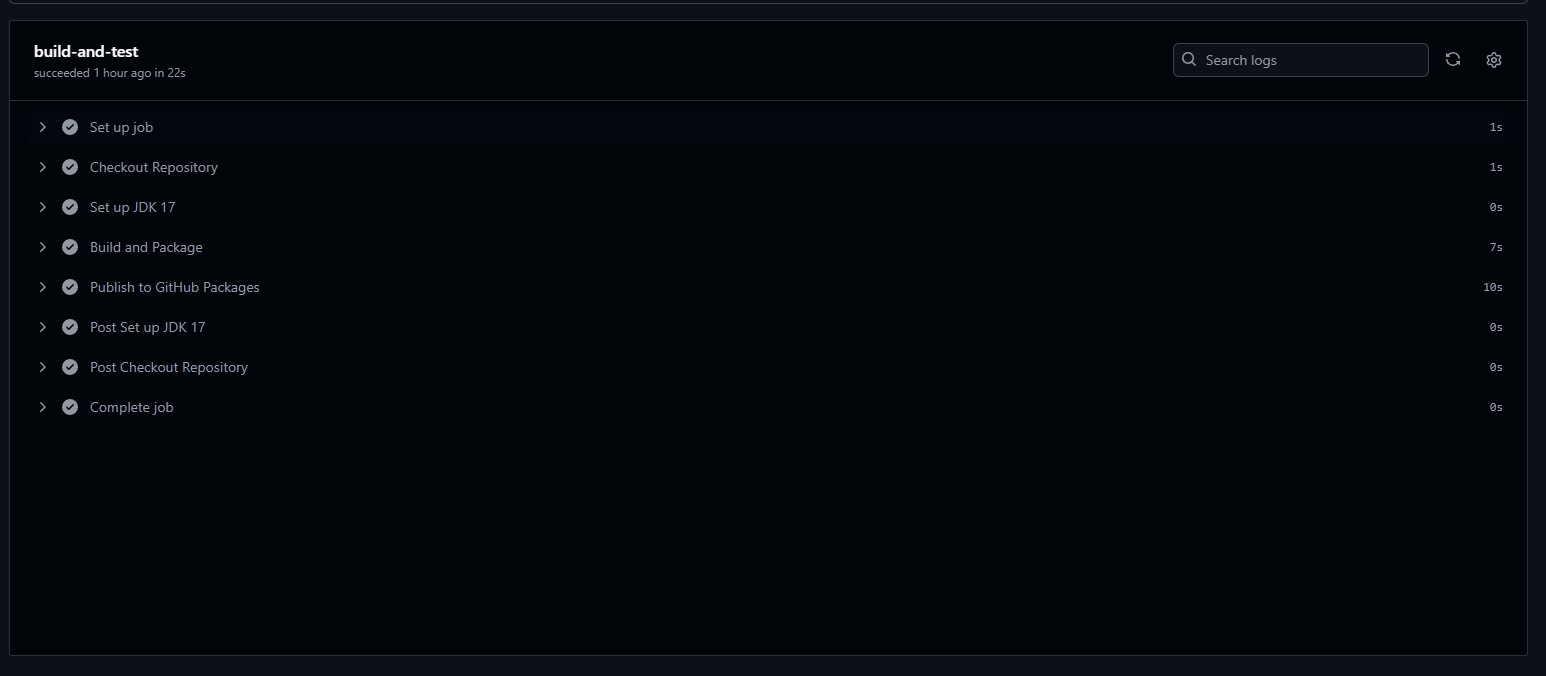
\includegraphics[width=\linewidth]{"C:/Users/laure/Documents/bachelorproef-2024-2025-laurensDeVos/graphics/Repo1Geslaagd.png"}
    \caption{Overzicht van een succesvolle uitvoering van de workflow in \texttt{Repo1}. Elke job is voltooid, zoals aangegeven door de vinkjes.}
    \label{fig:workflow-repo1}
\end{figure}

\chapter{Onderzoeksvoorstel}

Het onderwerp van deze bachelorproef is gebaseerd op een onderzoeksvoorstel dat vooraf werd beoordeeld door de promotor. Dat voorstel is opgenomen in deze bijlage.\\


%% TODO: 
%\section*{Samenvatting}

% Kopieer en plak hier de samenvatting (abstract) van je onderzoeksvoorstel.

% Verwijzing naar het bestand met de inhoud van het onderzoeksvoorstel
%==============================================================================
% Sjabloon onderzoeksvoorstel bachproef
%==============================================================================
% Gebaseerd op document class `hogent-article'
% zie <https://github.com/HoGentTIN/latex-hogent-article>

% Voor een voorstel in het Engels: voeg de documentclass-optie [english] toe.
% Let op: kan enkel na toestemming van de bachelorproefcoördinator!
\documentclass{hogent-article}

% Invoegen bibliografiebestand
\addbibresource{voorstel.bib}

% Informatie over de opleiding, het vak en soort opdracht
\studyprogramme{Professionele bachelor toegepaste informatica}
\course{Bachelorproef}
\assignmenttype{Onderzoeksvoorstel}
% Voor een voorstel in het Engels, haal de volgende 3 regels uit commentaar
% \studyprogramme{Bachelor of applied information technology}
% \course{Bachelor thesis}
% \assignmenttype{Research proposal}

\academicyear{2024-2025} % TODO: pas het academiejaar aan

% TODO: Werktitel
\title{Het verbeteren van compliance- en governancevereisten bij DocShifter, een gespecialiseerd bedrijf in documentconversietechnologie, door de praktische implementatie van DevSecOps, met een focus op klantgegevensbescherming en interne softwareontwikkelingsprocessen.}

% TODO: Studentnaam en emailadres invullen
\author{Laurens De Vos}
\email{laurens.devos@student.hogent.be}
\projectrepo{https://github.com/Laurensdevos2001/bachelorproef-2023-2024-laurensDeVos.git}

% TODO: Medestudent
% Gaat het om een bachelorproef in samenwerking met een student in een andere
% opleiding? Geef dan de naam en emailadres hier
% \author{Yasmine Alaoui (naam opleiding)}
% \email{yasmine.alaoui@student.hogent.be}

% TODO: Geef de co-promotor op
\supervisor{Johnno Van De Velde}

% Binnen welke specialisatierichting uit 3TI situeert dit onderzoek zich?
% Kies uit deze lijst:
%
% - Mobile \& Enterprise development
% - AI \& Data Engineering
% - Functional \& Business Analysis
% - System \& Network Administrator
% - Mainframe Expert
% - Als het onderzoek niet past binnen een van deze domeinen specifieer je deze
%   zelf
%
\specialisation{System \& Network Administrator}
\keywords{DevSecOps, security, automation}

\begin{document}
    
    \begin{abstract}
    
    DocShifter, een bedrijf gespecialiseerd in documentconversietechnologie, kampt met significante uitdagingen op het gebied van compliance en governance, vooral met betrekking tot de bescherming van klantgegevens en naleving van de Algemene Verordening Gegevensbescherming (AVG).
    
    Om deze uitdagingen aan te pakken, is een uitgebreide literatuurstudie uitgevoerd. Deze studie analyseert de specifieke activiteiten van DocShifter, de compliance- en governancevereisten waaraan het moet voldoen, en de mogelijke gevolgen van niet-naleving. Op basis van deze analyse is een methodologie ontwikkeld, waarin een nulmeting de huidige status van compliance en governance evalueert. Vervolgens worden DevSecOps-praktijken geïmplementeerd, waarna de impact op de naleving van regelgeving en gegevensbescherming wordt gemeten.
    
    De resultaten van dit onderzoek bieden waardevolle inzichten in de compliance- en governance-uitdagingen van DocShifter. Bovendien wordt een praktische oplossing voorgesteld die de efficiëntie en effectiviteit van de bedrijfsprocessen verbetert, wat bijdraagt aan een versterkte naleving van regelgeving en betere gegevensbescherming.
    
    
    \end{abstract}
    
    \tableofcontents
    
    % De hoofdtekst van het voorstel zit in een apart bestand, zodat het makkelijk
    % kan opgenomen worden in de bijlagen van de bachelorproef zelf.
    %---------- Inleiding ---------------------------------------------------------
    
    \section{Introductie}%
    \label{sec:introductie}

    In de hedendaagse digitale wereld is het voor bedrijven cruciaal om te voldoen aan strikte compliance- en governancevereisten, met name op het gebied van klantgegevensbescherming en interne softwareontwikkelingsprocessen. DocShifter, een vooraanstaande speler in documentconversietechnologie, wordt momenteel geconfronteerd met specifieke uitdagingen bij het naleven van de Algemene Verordening Gegevensbescherming (AVG). Deze uitdagingen hebben betrekking op het ontoereikend versleutelen van klantgegevens of het niet tijdig en snel genoeg updaten van software om aan de vereisten te voldoen, wat de organisatie blootstelt aan aanzienlijke risico's op legaal vlak.
    
    \noindent De huidige aanpak van DocShifter blijkt ontoereikend te zijn, omdat veiligheidsmaatregelen over het hoofd kunnen gezien worden door een minder goede aanpak van software uit te brengen. Dit roept de vraag op hoe DocShifter zijn compliance- en governancekaders kan versterken om beter te voldoen aan de AVG en andere relevante normen.
    
    \noindent De centrale onderzoeksvraag in dit onderzoek luidt dan ook: Hoe kan de implementatie van DevSecOps bijdragen aan het verbeteren van de\\ compliance- en governancevereisten van DocShifter, specifiek in het kader van de AVG? Deze vraag wordt opgesplitst in de volgende deelvragen:
    
    \begin{itemize}
        \item  Wat zijn de huidige tekortkomingen in de compliance- en governanceaanpak van DocShifter ten aanzien van de AVG? Welke risico's lopen zij door deze tekortkomingen?
    \end{itemize}
    
    \begin{itemize}
        \item  Hoe kunnen DevSecOps-praktijken specifiek bijdragen aan het verbeteren van de naleving van de AVG bij DocShifter? Welke methoden en tools zijn het meest geschikt voor deze implementatie?
    \end{itemize}
    
    \noindent Op basis van deze deelvragen worden de volgende doelstellingen geformuleerd:
    
    \begin{itemize}
        \item Het in kaart brengen van de huidige \\ compliance- en governance-uitdagingen bij DocShifter met betrekking tot de AVG.
    \end{itemize}
    
    \begin{itemize}
        \item Het ontwikkelen en voorstellen van een \\ DevSecOps-strategie die specifiek gericht is op het aanpakken van deze uitdagingen.
    \end{itemize}
    \begin{itemize}
        \item Het evalueren van de effectiviteit van deze strategie in termen van verbeterde compliance en gegevensbescherming.
    \end{itemize}
    
    \noindent Door een grondige analyse van deze uitdagingen en mogelijke oplossingen, streeft dit onderzoek ernaar om concrete aanbevelingen te doen die de efficiëntie en effectiviteit van de bedrijfsprocessen bij DocShifter zullen verbeteren.
    
    
    
    
    %---------- Stand van zaken ---------------------------------------------------
    
   \section{Literatuurstudie}%
   \label{sec:literatuurstudie}
   \subsection{Inleiding tot DevSecOps en Compliance}
   DevSecOps, een samenvoeging van development, security en operations, is een benadering die beveiliging integreert als een gedeelde verantwoordelijkheid gedurende de volledige \\ IT-levenscyclus. Volgens Red Hat (2020) gaat dit concept verder dan het traditionele DevOps-model door beveiliging te betrekken vanaf de vroegste stadia van ontwikkeling en doorlopend tot de eindfase van het project.
   Traditioneel werd beveiliging vaak gezien als een afzonderlijke taak die pas aan het einde van het ontwikkelingsproces werd uitgevoerd. Met de toegenomen behoefte aan snellere ontwikkelingscycli in DevOps, is het echter cruciaal geworden om beveiliging continu en integraal te maken in het gehele proces. Dit betekent dat beveiligingsteam vanaf het begin betrokken zijn bij het project, en dat beveiligingscontroles worden geautomatiseerd en geschikte tools worden geselecteerd.
   De nadruk van DevSecOps ligt op het belang van vroegtijdige en doorlopende beveiliging. Dit benadrukt niet alleen het belang van het automatiseren van beveiligingscontroles, maar ook de noodzaak om beveiligingsteams vanaf het begin van het ontwikkelingsproces te betrekken.
   Effectieve implementatie van DevSecOps vereist dat beveiliging wordt geïntegreerd gedurende de volledige levenscyclus van applicaties. Automatisering speelt een cruciale rol in het vereenvoudigen van repetitieve taken en het handhaven van de ontwikkelingssnelheid. Bovendien breidt DevSecOps zich uit naar moderne technologieën zoals containers en microservices, die aangepaste beveiligingspraktijken vereisen om \\ applicatie- en infrastructuurbeveiliging te waarborgen \autocite{redhat2023}.
   
   \subsection{Belang van governance en compliance in DevSecOps}
   
  In DevSecOps is governance van cruciaal belang om ervoor te zorgen dat beveiliging en compliance geïntegreerd worden binnen de ontwikkelings- en operationele processen. Dit gaat verder dan alleen het toevoegen van beveiligingscontroles; het vereist een gestructureerde benadering waarbij beleidsregels, standaarden en compliance-eisen consistent worden nageleefd en toegepast in de volledige softwarelevenscyclus.
  
  Een Gartner-enquête uit 2022 toonde aan dat 90\% van de organisaties de noodzaak ziet om governance en compliance te verbeteren door een betere integratie van beveiligingsoperaties \autocite{GlobalSign2022}. DevSecOps maakt dit mogelijk door beveiligingscontroles vroeg in de softwareontwikkelingscyclus te integreren, waardoor risico's beter beheerst kunnen worden en compliance automatisch kan worden gehandhaafd. Traditioneel werden beveiliging en compliance als losse stappen aan het einde van een ontwikkelproces toegevoegd, wat vaak leidde tot vertragingen en hoge kosten. Met DevSecOps worden beveiliging en compliance echter onderdeel van het ontwikkelproces, waardoor problemen vroegtijdig kunnen worden opgespoord en opgelost.
  
  Volgens de OWASP DevSecOps-richtlijnen is het hanteren van een "shift-left" benadering een sleutelelement van governance binnen DevSecOps. Deze benadering houdt in dat beveiligings- en complianceactiviteiten al vroeg in het ontwikkelproces worden geïmplementeerd, bijvoorbeeld tijdens het coderen en testen. Dit verkleint niet alleen de kans op beveiligingsincidenten, maar zorgt ook voor een continue naleving van regelgeving gedurende de hele levenscyclus van de applicatie.\autocite{Project2019}
  
  Kortom, goede governance in DevSecOps stelt organisaties in staat om de naleving van regelgeving en beveiligingsstandaarden effectief te waarborgen. Dit verbetert niet alleen de veiligheid van softwaretoepassingen, maar helpt ook bij het voldoen aan wettelijke en industriële normen zoals ISO 27001 en AVG, wat essentieel is voor organisaties die opereren in gereguleerde sectoren.
  
   
   \subsection{Automatisering van compliance binnen DevSecOps}
   
   Automatisering speelt een cruciale rol in het handhaven van compliance binnen DevSecOps volgens Odorfer (2021). Door beleid als code (policy as code) te implementeren, kunnen organisaties de naleving van beveiligingsnormen en -procedures op een consistente en schaalbare manier waarborgen. Volgens de AWS Security Blog stelt beleid als code teams in staat om beveiligings- en compliance-eisen te automatiseren door regels in code te definiëren, die vervolgens automatisch kunnen worden toegepast en gecontroleerd in de ontwikkelings- en operationele processen.
   
   Deze aanpak minimaliseert niet alleen menselijke fouten, maar zorgt ook voor een snellere feedbacklus, waardoor teams proactief kunnen reageren op compliance-issues voordat ze problematisch worden. Door tools en technologieën in te zetten die beleidsregels automatisch toepassen, kunnen organisaties de risico's van niet-naleving verlagen en de snelheid van softwarelevering verhogen, wat cruciaal is in de huidige snel veranderende digitale omgeving.
   
   Bovendien maakt de automatisering van compliance het mogelijk om voortdurend te monitoren en rapporteren over de naleving, waardoor teams beter in staat zijn om te voldoen aan zowel interne beleidslijnen als externe regelgeving, zoals de AVG en andere industriestandaarden.\autocite{Odorfer2021}
   
   \subsection{Specifieke regelgeving en standaarden relevant voor DevSecOps}
   
  In het kader van DevSecOps is het essentieel om op de hoogte te zijn van specifieke regelgeving en standaarden die invloed hebben op de ontwikkeling en het beheer van softwareapplicaties. Een belangrijke wetgeving in Europa is de Algemene Verordening Gegevensbescherming (AVG), die strikte richtlijnen biedt voor de bescherming van persoonlijke gegevens. De AVG verplicht organisaties om passende technische en organisatorische maatregelen te nemen om de privacy van klanten te waarborgen en hen te beschermen tegen gegevensinbreuken .
  
  De AVG legt ook de verantwoordelijkheid bij organisaties om transparant te zijn over hoe ze gegevens verzamelen, opslaan en verwerken. Dit is cruciaal voor DevSecOps-teams, aangezien zij beveiliging en compliance in de vroege stadia van de softwarelevenscyclus moeten integreren. Door de richtlijnen van de AVG te volgen, kunnen organisaties niet alleen hun juridische verplichtingen nakomen, maar ook het vertrouwen van klanten vergroten door transparante en veilige gegevensverwerking.
  
  Bovendien kunnen DevSecOps-teams profiteren van best practices en richtlijnen van andere organisaties, zoals de Open Web Application Security Project (OWASP), die helpen bij het implementeren van veilige ontwikkelingspraktijken en het handhaven van compliance met relevante regelgeving.
  \autocite{EU2022}
  
  \subsection{Best practices voor compliance-gedreven DevSecOps-implementatie}
  
  Volgens OWASP (2021) is het implementeren van best practices voor compliance-gedreven DevSecOps essentieel voor het effectief integreren van beveiliging en compliance binnen de softwareontwikkelingslevenscyclus. Volgens de OWASP DevSecOps Guideline moeten organisaties een proactieve aanpak hanteren die gericht is op het integreren van beveiligingsmaatregelen in alle fasen van de ontwikkeling. Dit betekent dat beveiliging niet als een afzonderlijke stap aan het einde van het ontwikkelingsproces moet worden gezien, maar als een continu proces dat begint met de planningsfase en zich uitstrekt tot en met de implementatie en het onderhoud van de software.\autocite{OWASP2021}
  
  Een belangrijk aspect van deze proactieve benadering is het automatiseren van beveiligingscontroles en compliance-eisen. Puppet benadrukt het belang van automatisering in hun blog over een proactieve beveiligingsaanpak, waarbij ze aangeven dat automatisering helpt bij het minimaliseren van menselijke fouten en het versnellen van het compliance-proces (Puppet, 2022). Dit maakt het mogelijk om consistentie en betrouwbaarheid in beveiligingsmaatregelen te waarborgen en snel te reageren op eventuele compliance-issues die zich kunnen voordoen.\autocite{Puppet2022}
  
  Red Hat wijst ook op het belang van een integrale DevSecOps-aanpak, waarbij samenwerking tussen ontwikkeling, beveiliging en operaties wordt bevorderd. Dit bevordert een cultuur van gezamenlijke verantwoordelijkheid voor beveiliging en compliance, wat essentieel is voor het succes van een DevSecOps-implementatie (Red Hat, 2023). Door teams in staat te stellen om samen te werken en gedeelde doelen te hebben, kunnen organisaties beter inspelen op de voortdurende veranderingen in regelgeving en beveiligingseisen.\autocite{RedHat2021}
  
  
  
  
  
    
    %---------- Methodologie ------------------------------------------------------
    \section{Methodologie}%
    \label{sec:methodologie}
    
    \noindent Om de implementatie van DevSecOps te onderzoeken met een focus op governance- en compliancevereisten, wordt de methodologie voorgesteld die uit drie fasen bestaat. 
    
    \subsection{Fase 1: Analyse van huidige compliance- en governancevereisten}
    \noindent De eerste fase omvat een grondige analyse van de huidige compliance- en governancevereisten van DocShifter. Dit proces zal inhouden:
    
    \begin{itemize}
        \item Stakeholder interviews: Het uitvoeren van interviews met een select aantal relevante stakeholders, zoals ontwikkelaars en DevOps-engineers, om hun ervaringen en percepties van de huidige compliance-eisen te verzamelen.
        \item Procesanalyse: Gelijktijdig met de interviews worden de bestaande processen en workflows binnen DocShifter in kaart gebracht om inefficiënties en risico’s te identificeren.
    \end{itemize}
    
    \subsection{Fase 2: Literatuurstudie}
    \noindent Een literatuurstudie wordt uitgevoerd die specifiek ingaat op de governance- en compliancevereisten, met nadruk op:
    
    \begin{itemize}
        \item Best Practices en Case Studies: Het identificeren van best practices en relevante case studies die specifiek gericht zijn op de geïdentificeerde vereisten. Deze inzichten zullen helpen bij het vormen van een solide basis voor de implementatie van DevSecOps.
    \end{itemize}
    
    \subsection{Fase 3: Evaluatie en Aanbevelingen}
    \noindent Op basis van de inzichten uit de literatuurstudie en de eerdere analyse worden aanbevelingen gedaan voor de implementatie van DevSecOps binnen DocShifter. Dit omvat:
    
    \begin{itemize}
        \item Longlist en Shortlist van Oplossingen: Het opstellen van een shortlist van tools en frameworks die kunnen bijdragen aan de governance en compliance, inclusief een evaluatie op effectiviteit en toepasbaarheid.
        \item Proof of Concept: Het uitvoeren van een beperkte implementatie van de geselecteerde oplossingen om de haalbaarheid en effectiviteit in de praktijk te testen.
    \end{itemize}
    
    %---------- Verwachte resultaten ----------------------------------------------
    \section{Verwacht resultaat, conclusie}%
    \label{sec:verwachte_resultaten}
    Het onderzoek zal naar verwachting resulteren in een diepgaand inzicht in de huidige compliance- en governance-uitdagingen van DocShifter. Door middel van een systematische analyse en literatuurstudie wordt verwacht dat er een duidelijke strategie zal worden ontwikkeld voor de implementatie van DevSecOps binnen het bedrijf. Deze strategie resulteert in een selectie van relevante tools en best practices die specifiek zijn afgestemd op de behoeften van DocShifter. Bovendien zal de Proof of Concept een praktisch bewijs leveren van de effectiviteit van deze aanpak, wat zal bijdragen aan het verbeteren van interne processen.
    
    In conclusie zal dit onderzoek waardevolle inzichten bieden in hoe DocShifter zijn compliance- en governancevereisten kan versterken door de implementatie van DevSecOps. De voorgestelde oplossingen zullen niet alleen de huidige uitdagingen aanpakken, maar ook een duurzame basis leggen voor toekomstige verbeteringen in de beveiliging en efficiëntie binnnen DocShifter. De resultaten van dit onderzoek zullen DocShifter in staat stellen om beter te voldoen aan relevante regelgeving, wat uiteindelijk zal bijdragen aan een versterkt vertrouwen van klanten en stakeholders.
    
    
         
    
    \printbibliography[heading=bibintoc]
    
\end{document}

%%---------- Andere bijlagen --------------------------------------------------
% TODO: Voeg hier eventuele andere bijlagen toe. Bv. als je deze BP voor de
% tweede keer indient, een overzicht van de verbeteringen t.o.v. het origineel.
%\input{...}

%%---------- Backmatter, referentielijst ---------------------------------------

\backmatter{}

\setlength\bibitemsep{2pt} %% Add Some space between the bibliograpy entries
\printbibliography[heading=bibintoc]

\end{document}
